% Florian Sihler, 2022
% Licensed under GNU General Public License version 3
% https://opensource.org/licenses/gpl-3.0.html
\errorcontextlines9999
\documentclass[parskip=half,english,numbers=noenddot,footnotes=nomultiple,oneside]{scrartcl}

\usepackage[T1]{fontenc}
\usepackage[utf8]{inputenc}
\usepackage{babel}

\makeatletter\def\input@path{{../tex/}}\makeatother
\usepackage[glows]{tikzpingus}

% \definecolor{doc-main}{RGB}{204,0,25}
\colorlet{@opcolor}{pingu@blue!75!black}
\colorlet{doc-main}{@opcolor!80!pingu@black}
\usepackage[linkcolor=@opcolor,urlcolor=@opcolor,colorlinks,breaklinks,pdfusetitle]{hyperref}
\usetikzlibrary{shapes.misc,arrows.meta}
\urlstyle{same}
\expandafter\def\expandafter\UrlBreaks\expandafter{\UrlBreaks\do-}

\usepackage[tex,hyper]{listings}
\usepackage[skins,breakable,hooks,xparse,listingsutf8,external]{tcolorbox}
\usepackage{lmodern}
\usepackage{CrimsonPro}

\usepackage{imakeidx}
\usepackage{tikz}
\usepackage{fontawesome}
\usepackage{csquotes}
\usepackage{enumitem}
\usepackage{microtype}
\usepackage{tikzducks}
\usepackage{datatool}
\usepackage{relsize}
\usepackage{multicol}
\usepackage{footnotebackref}
\usepackage{adjustbox}
\usepackage{xstring}
\usepackage{colorinfo}

\makeindex[title={Key Overview},columns=2,columnsep=.75cm,noautomatic=true,options=-s indexstyle.ist]
\deffootnote{1.5em}{1em}{\textsuperscript{\hyperref[\BackrefFootnoteTag]{\thefootnotemark}}\thinspace}
\def\thefootnote{$\langle$\arabic{footnote}$\rangle$}
% https://tex.stackexchange.com/questions/78423/how-to-use-the-footnotebackref-package-with-footnotemark-and-footnotetext
\makeatletter
\LetLtxMacro\BHFN@Old@footnotemark\@footnotemark
\def\@footnotemark{%
    \refstepcounter{BackrefHyperFootnoteCounter}%
    \xdef\BackrefFootnoteTag{bhfn:\theBackrefHyperFootnoteCounter}%
    \label{\BackrefFootnoteTag}%
    \BHFN@Old@footnotemark
}

\newlist{inlist}{enumerate*}{1}
\setlist[inlist]{itemjoin={{, }},itemjoin*={{, and }},label=$\roman*$),mode=boxed}

\let\say\enquote
\def\DTLlistformatoxford{,}\def\DTLandname{and}
% TODO: do guard against same keys for different selectors
\long\def\ParseDTLListElement#1"#2"\@nil{\textsuperscript{\smash{\raisebox{2pt}{\ifcsname pingu@@lib@#2@\CurrentList @\endcsname\index{Libraries!\textit{\csname pingu@@lib@#2@\CurrentList @\endcsname}!#2?\hyperref[expl-list:\CurrentList]{\protect\lpingu{#2} {\tiny\sffamily(\CurrentList)}~$\underset{\text{\tiny\smash{\raisebox{3pt}{\textsf{\hyperref[Libraries]{\color{gray}Library}}}}}}{\text{\textit{\tiny\strut\csname pingu@@lib@#2@\CurrentList @\endcsname}}}$\fi}}}}
\def\DTLlistformatitem#1{\textit{#1\expandafter\ParseDTLListElement :#1\@nil}}
\newcommand*\typesetselection[1][]{\begingroup\ifx!#1!\else\def\DTLlistformatitem##1{#1}\fi\dotypesetselection}
\def\dotypesetselection#1{\label{expl-list:#1}\def\CurrentList{#1}\expandafter\DTLformatlist\expandafter{\csname @pingu@#1@\endcsname}\endgroup}
\makeatletter

\addtokomafont{sectioning}{\@declaredcolor{gray}}
\addtokomafont{title}{\@declaredcolor{doc-main}}
\addtokomafont{author}{\normalsize}
\addtokomafont{date}{\normalsize}

\def\optstyle{\@declaredcolor{@opcolor}\slshape}
\colorlet{@softgray}{gray!60!white}
\colorlet{@softgray@b}{gray!75!white}
\colorlet{@darkerblue}{pingu@blue!40!black}
\def\lstfnsize{-.7}
\lstdefinestyle{lstpingu}{%
	tabsize=2, breaklines,
	basicstyle=\relsize{\lstfnsize}\ttfamily,
	commentstyle={\@declaredcolor{gray}\slshape},
	columns=fullflexible,
	emphstyle=\slshape,
	emphstyle=[2]\optstyle,
	emphstyle=[3]\@declaredcolor{@softgray@b},
	emphstyle=[4]\@declaredcolor{@darkerblue},
	texcsstyle=*\@declaredcolor{gray}\bfseries,
	texcsstyle=*[2]\@declaredcolor{doc-main}\bfseries,
	texcsstyle=*[3]\@declaredcolor{@softgray},
	lineskip=2.5pt,
	keepspaces=true,
	moredelim=[s][\itshape]{<}{>},
}
\lstset{style=lstpingu}
\def\ipingu#1{\lstinline'#1'}
\def\lpingu#1{\lstinline[style=lstpingu,language=pingulang]'#1'}
\def\ltex#1{\lstinline[style=lstpingu,language=pinguinternallang]'#1'}

\lstdefinelanguage{pinguinternallang}{
	language={[LaTeX]TeX},
	moreemph={tikzpicture},
	alsoletter={@},
	moretexcs=[2]{pingu@block,pingu@draw},
	moretexcs={pingu@eye@shift,pingu@color@eye@left,pingu@color@eye@right,pingu@name,@pingu@eyes@s,@pingu@none}
}

\def\t@lst@addToLiterate#1{\protected@edef\lst@literate{\unexpanded\expandafter{\lst@literate}\unexpanded{#1}}}
\lst@Key{add to literate}{}{\t@lst@addToLiterate{#1}}
\let\lst@ifxliterate\iftrue % make literate a star literate

\lstdefinelanguage{pingulang}{
	language={[LaTeX]TeX},
	moreemph={tikzpicture},
	alsoletter={.-!:0123456789},%disable number
	deletetexcs={begin,end}, % -> lift 3
	moretexcs=[2]{pingu,duck,node,pingudefaults,pingudefaultsappend,pinguloadlibrary,pinguloadlibraries},
	moretexcs=[3]{begin,end,pgfmathsetseed},
	moreemph=[3]{!hide,.style},
	add to literate={/pingu/}{{\@declaredcolor{gray}/pingu/}}7
		{\{tikzpicture\}}{{\@declaredcolor{@softgray}\{tikzpicture\}}}{13}
		{\{\\number\\pdfrandomseed\}}{{\@declaredcolor{@softgray}\{\textbackslash number\textbackslash pdfrandomseed\}}}{23}
		% otherwise these would interfere with random
		{!random}{{\@declaredcolor{darkgray}\itshape!random}}7
}

\def\@CreateCodeHyperLink#1#2#3{\lstset{add to literate={#2}{{\hyperref[#3]{\optstyle#2}}}{#1}}}
% #1 Keys | #2 length (optimized)
\def\CreateCodeHyperLink#1#2{% \StrLen{\@elem}[\@cclen]
	\@for\@elem:=#1\do{\ifx\@elem\@empty\else
	% space to space cmd % TODO: do this on store and just keep store?
	\StrSubstitute{\@elem}{ }{\noexpand\ }[\@sub]\relax
	\edef\@tmp{\noexpand\@CreateCodeHyperLink{#2}{\@sub}{pk:/pingu/\@elem}}\@tmp\fi}%
}
% store all. we use their precalculated length to ensure prefixes we go from small to large on set
\def\cmdsstore#1#2{\csxdef{allcmds@#1}{#2}}
\def\allcmdsmin{3}% think
\def\allcmdsmax{3}%
\AtEndDocument{%
	\pgfkeys{/pingu/.cd,defaults}% this way we have active defaults
	\foreach \i in {\allcmdsmin,...,\allcmdsmax} {%
		\immediate\write\@auxout{\noexpand\cmdsstore{\i}{\csuse{allcmds@\i}}}%
	}%
	\immediate\write\@auxout{%
		\noexpand\gdef\noexpand\allcmdsmin{\allcmdsmin}%
		\noexpand\gdef\noexpand\allcmdsmax{\allcmdsmax}%
		\noexpand\gdef\noexpand\pengu@all@showcases{\pengu@all@showcases}%
	}%
}


\def\RawShowcase#1#2{\scalebox{.68}{%\begin{tcbexternal}{showcase-#2#1}%
\tikzpicture[baseline={(pingu-bottom-center)}]
\pingu[body=pingu@main!30!white,bill color=pingu@yellow!30!white,feet color=pingu@yellow!30!white,eyes color=pingu@black!30!white,name=pingu,#1#2]
\pgfonlayer{foreground}
\node[below=3mm] at(pingu-bottom-center) {\strut}; % buffer
\pgfinterruptboundingbox
\node[below=3mm,fill=white,fill opacity=.52,text opacity=1,rounded corners=1pt] at(pingu-bottom-center) {\textsf{\strut\smash{#1}}};
\endpgfinterruptboundingbox
\endpgfonlayer
\endtikzpicture
%\end{tcbexternal}%
}}

\setbox0=\hbox{\RawShowcase{}{}}
\newdimen\pingu@showcase@height
\pingu@showcase@height=\dimexpr\ht0+\dp0\relax

\def\ShowcasePengu#1=#2;{{\hypersetup{linkcolor=.}%
\hyperref[pk:/pingu/#1]{%
	\parbox[b][\pingu@showcase@height]{.14\linewidth}{\centering\ifx!#2!\def\Arg{}\else\def\Arg{=#2}\fi\edef\MakeShowcase{\noexpand\RawShowcase{#1}{\Arg}}~\clap{\MakeShowcase}~}%
}}}
\def\pengu@all@showcases{}
% we mix them somewhat funny
\def\@showcase@pre{pre}
\let\@showcase@cur\@showcase@pre
\def\@toggle@showcase{\ifx\@showcase@cur\@showcase@pre\global\let\@showcase@cur\@empty\else \global\let\@showcase@cur\@showcase@pre\fi}
\newcommand\ShowcaseThis[2][]{\ifx\@showcase@cur\@showcase@pre \global\let\@showcase@cur\@empty\expandafter\gpreto\else \global\let\@showcase@cur\@showcase@pre\expandafter\gappto\fi\pengu@all@showcases{{#2=#1},}}

\RedeclareSectionCommand[runin=false,afterskip=-2mm]{section}
\RedeclareSectionCommand[runin=false,afterskip=-2mm]{subsection}

\tcbset{%
	colframe=gray,enhanced,breakable, arc=2mm,
	fonttitle=\bfseries, sidebyside,
	boxrule=.35mm,listing options={style=lstpingu,language=pingulang},
	center lower,segmentation at break=false,
	righthand width=4.75cm, bottom=0pt, top=0pt,boxsep=2.25pt,
	before lower app={}, colback=white
}
\lstMakeShortInline[style=lstpingu,language=pingulang,basicstyle=\relsize{-1}\ttfamily\@declaredcolor{black!90!white},moredelim={[s][\itshape]{<}{>}}]{|}

\def\explaincolor{@opcolor!8!white}
\def\cursub{}
\def\keyexplainindent{2.5em}%
% allow the oxes to have minor overlaps
\newenvironment{keyexplain}[4][/pingu/]{\minipage{\linewidth}
	\parskip\smallskipamount
	\StrSubstitute{#2}{ }{-}[\keyexternalname]%
	\tcbset{@/.style={externalize listing=key-\keyexternalname}}% set for externalize
	\phantomsection\label{pk:#1#2}\index{\cursub#2?\hyperref[pk:#1#2]{\protect\lpingu{#2}}}%
	% get its length:
	\StrLen{#2}[\@cclen]%
	\csgappto{allcmds@\@cclen}{#2,}%
	% update the range
	\ifnum\@cclen>\allcmdsmax\relax \xdef\allcmdsmax{\@cclen}\fi
	\ifnum\@cclen<\allcmdsmin\relax \xdef\allcmdsmin{\@cclen}\fi
	\expandafter\gdef\csname pinguopt#2\endcsname{#3}%
	\expandafter\gdef\csname pingudefa#2\endcsname{#4}%
	\begingroup\pgfkeys{/pingu/.cd,defaults}\protected@edef\@tmp{#4}%
	\protected@edef\@tmpb{#3}%
	\hspace*{-\keyexplainindent}\tcbox[left=3pt,right=3pt,top=3pt,bottom=3pt,colframe=white,colback=\explaincolor,on line]{%
		\parbox{\dimexpr\linewidth-2\fboxsep+\keyexplainindent}{\small
		\ifx\@tmpb\@empty\lpingu{#1#2}\else\lpingu{#1#2 =\ }\texttt{<\textit{\@tmpb}>}\fi\hfill
				\ifx\@tmp\@empty\else{\@declaredcolor{gray}(}#4{\@declaredcolor{gray})}\fi
		}
	}\ifcsname pingu@@lib@#2@\endcsname\index{Libraries!\textit{\csname pingu@@lib@#2@\endcsname}!#2?\hyperref[pk:#1#2]{\protect\lpingu{#2}}}\rlap{~\quad\raisebox{3pt}{$\underset{\text{\tiny\smash{\raisebox{3pt}{\textsf{\hyperref[Libraries]{\color{gray}Library}}}}}}{\text{\textit{\footnotesize\strut\csname pingu@@lib@#2@\endcsname}}}$}}\fi\par\endgroup
}
{\endminipage\smallskip\par}

\def\singleshortcut#1#2"#3"#4{\def\cursub{#2?\hyperref[pk:#1#2]{\protect\lpingu{#2}}!}\keyexplain[#1]{#2 #3}{\csname pinguopt#4\endcsname}{\csname pingudefa#4\endcsname}%
	\textcolor{gray}{\footnotesize This is a shortcut for: \texttt{\keyref[#1]{#2}\relsize{-1}{\ =\ {\optstyle#3}}}. The \enquote{\texttt{\textit{\csname pinguopt#4\endcsname}}} argument is passed to \keyref[#1]{#4}.}
\endkeyexplain}
\newcommand*\shortcuts[4][/pingu/]{\begingroup
\protected@edef\@tmp{#3}%
\def\explaincolor{@softexplaincolor}%
\foreach \type in \@tmp {%
\edef\tmp{\noexpand\singleshortcut{#1}{#2}\type{#4}}\tmp
}\endgroup}

\newcommand*\keyref[2][/pingu/]{\hyperref[pk:#1#2]{\lpingu{#1#2}}}
\newcommand*\dkeyref[2][/pingu/]{\hyperref[pk:#1#2]{\lpingu{#2}}}
\colorlet{@softexplaincolor}{gray!8!white}
\newenvironment{subkeyexplain}[5][/pingu/]{%
\begingroup
\def\explaincolor{@softexplaincolor}\def\keyexplainindent{0em}%
\def\cursub{#2?\hyperref[pk:#1#2]{\protect\lpingu{#2}}!}%
\keyexplain[#1]{#3}{#4}{#5}%
	{\@declaredcolor{gray}\footnotesize This command is only in effect if \keyref[#1]{#2} is active.}\par
}{\endkeyexplain\endgroup}

\def\consumeshowkeyexplain#1(#2){\ShowcaseThis[#2]{#1}}
\newenvironment{showkeyexplain}[4][/pingu/]{%
\keyexplain[#1]{#2}{#3}{#4}%
\@ifnextchar({\consumeshowkeyexplain{#2}}{\consumeshowkeyexplain{#2}()}
}{\endkeyexplain}

\newcommand\keyalias[3][/pingu/]{\begingroup
\def\explaincolor{@softexplaincolor}\def\keyexplainindent{0em}%
\def\cursub{#3?\hyperref[pk:#1#3]{\protect\lpingu{#3}}!}%
\keyexplain[#1]{#2}{\csname pinguopt#3\endcsname}{\csname pingudefa#3\endcsname}%
	{\@declaredcolor{gray}\footnotesize This is an alias for \keyref[#1]{#3}.}%
\endkeyexplain\endgroup}
\newcommand\subkeyalias[4][/pingu/]{\begingroup
\def\explaincolor{@softexplaincolor}\def\keyexplainindent{0em}%
\def\cursub{#4?\hyperref[pk:#1#4]{\protect\lpingu{#4}}!#3?\hyperref[pk:#1#3]{\protect\lpingu{#3}}!}%
\keyexplain[#1]{#2}{\csname pinguopt#3\endcsname}{\csname pingudefa#3\endcsname}%
	{\@declaredcolor{gray}\footnotesize This is an alias for \keyref[#1]{#3}.}%
\endkeyexplain\endgroup}

\def\lib#1{\tikz[baseline=-.6ex]\node[draw=teal,fill=teal!3!white,very thick,rounded corners=2pt,inner ysep=0pt]{\sffamily\strut#1};}

\def\TikZ{Ti\textit{k}Z}
\def\tikzpingus{\TikZ pingus}

\tcbset{external/prefix=sub_}
\tcbEXTERNALIZE % we do not need the other configurationshttps://www.freecodecamp.org/news/deploy-a-react-app-to-github-pages/ in the externalized images :D

\hfuzz=12pt

% this should not happen in the external images
\AtBeginDocument{%
% we do not use foreach to avoid groups
\count@=\allcmdsmin
\edef\@cntmax@{\the\numexpr\allcmdsmax+1\relax}%
\@whilenum\count@<\@cntmax@\do{%
	\edef\i{\number\count@}\relax
	\ifcsname allcmds@\i\endcsname
		\edef\allcmds{\csname allcmds@\i\endcsname}% if undefined => empty
		\expandafter\CreateCodeHyperLink\expandafter{\allcmds}{\i}%
		\csxdef{allcmds@\i}{}%
	\fi% csx kill to stop infinite
	\global\advance\count@\@ne
}%
}
\def\TypesetShowcases{\@tempcnta\z@
\begingroup\parskip\z@ \parindent\z@
\@for\@elem:=\pengu@all@showcases\do{%
	\advance\@tempcnta\@ne
	\ifnum\@tempcnta>5 \global\@tempcnta\@ne\par\fi
	\ifx\@elem\@empty\else
	% space to space cmd
	\edef\@tmp{\noexpand\ShowcasePengu\@elem;}\hfill\@tmp\hfill
\fi}%
\endgroup\global\let\pengu@all@showcases\@empty}

\def\PenguinTitle{%
\setbox0=\hbox{\tikz{\pingu[body type=tilt-right,eyes wink,conical hat,cane right,bow tie=pingu@purple,left wing grab,cup=doc-main]}}%
\begin{tikzpicture}[overlay,remember picture]
	\node[below left=1.5cm,rotate=-10] at (current page.north east) {\box0};
\end{tikzpicture}%
}

\title{The \texorpdfstring{\tikzpingus}{tikzpingus} package}
% \subtitle{Penguins with \TikZ}
\author{%
	\texorpdfstring{Florian Sihler\\*
		\url{https://github.com/EagleoutIce/tikzpingus}
	}{Florian Sihler}}
\date{Version v1.0 \textendash\ 2022/08/14}

\begin{document}
\maketitle
\PenguinTitle

\begingroup
\vspace*{-4em}\newsavebox\pinguboxA
\savebox\pinguboxA{\tikz{\pingu[wings raise,santa hat,eyes wink,bow tie=pingu@yellow]}}
\newsavebox\pinguboxB
\savebox\pinguboxB{\tikz{\pingu[wings raise,head band,eyes angry,sunglasses,bow tie=doc-main,body type=chubby]}}
\begin{center}
\begin{tikzpicture}
    \node[text width=.95\linewidth, inner sep=11pt] (m) {%
	 For my slides at university, I started to use the famous \LaTeX-package \textsl{\href{https://github.com/samcarter/tikzducks}{tikzducks}} a few years ago.
	 Yet, it seemed somewhat of a necessity to extend the range of available \say{cute} animals in \LaTeX.
	 Therefore I started writing this package: \textsl{tikzpingus}.\footnotemark\medskip\\
	 \textit{Please note:} While tikzpingus is certainly inspired by tikzducks, it does offer a different set of features (e.g., multiple wing positions,~\ldots).\medskip\\
	 I would be happy for any feedback or issues on the \href{https://github.com/EagleoutIce/tikzpingus}{tikzpingus}-GitHub.
    };
\pgfonlayer{background}
    \node[below,xshift=1.1cm,yshift=19.5pt,scale=.4] at(m.south west) {\usebox\pinguboxA};
    \node[below,xshift=-1cm,yshift=13.5pt,scale=.4] at(m.south east) {\usebox\pinguboxB};
    \draw[rounded corners,gray,fill=white] (m.north west) -- (m.north east) -- (m.south east) -- ++(-.45cm,0) to[bend right=40] ++(-1.2cm,0) -- ([xshift=1.65cm]m.south west) to[bend right=40] ++(-1.2cm,0) -- ++(-.45cm,0) -- cycle;
	 \endpgfonlayer
	 \node[above=3mm,font=\bfseries\sffamily\Large] at(current bounding box.north) {Motivation};
\end{tikzpicture}\vspace*{-\baselineskip}
\end{center}
\footnotetext{Why \say{pingu} and not \say{pengu}? Well, this is the third try on achieving cute penguins without using any templates or vector formats as a basis. As a german, the short form \say{pingu} was merely a typo that originated from the german word \say{pinguin} for \say{penguin}. It somewhat sticked\ldots}
\endgroup\vfill

\begin{center}
	\newsavebox\pinguA \newsavebox\pinguB \newsavebox\pinguC \newsavebox\pinguD \newsavebox\pinguE \newsavebox\pinguF \newsavebox\pinguG
	\def\Table#1(#2)#3{\scope[shift={(#2)},xshift=1.75cm,yshift=1.75cm]\pingu[#1]\endscope\pgfonlayer{foreground}\draw[lightgray,line width=6pt,rounded corners=2pt,line cap=round](#2) |- ++(4.5,1.35) -- ++(0,-1.35);\fill[draw=lightgray,fill=white,line width=3pt,rounded corners=2pt] (#2)++(3pt-1.5pt,-3pt+1.5pt+2mm) rectangle ++(1.15,1.15) node[midway,centered]{\Large$\mathsf{#3}$};\endpgfonlayer}%
	\setbox\pinguA=\hbox{\tikz{\pingu[santa hat,santa beard,eyes vertical,blush]}}%
	\setbox\pinguB=\hbox{\tikz{\pingu[:back,right wing wave,rook=pingu@silver!80!white,rook hatch=false]}}%
\resizebox*!{4.5cm}{\begin{tikzpicture}
\Table{right wing wave,horse right,crown, eyes wink, crown position={1:(-.1cm,-.255cm){1.33}}}(2.5,3.5){\text{\sffamily f}(x)}
\Table{right wing wave,eyes wink,shirt=gray,tie,blush}(0,0)+
\Table{right wing wave,eyes vertical,cloak=gray,body type=legacy,cup,left wing grab,blush}(5,0)*

\Table{right wing wave,left wing shock,eyes shock,halo,heart=gray!40!pingu@white}(-2.5,-4)\div
\Table{right wing wave,cake-hat,eyes wink,flag right}(2.5,-4)\ln
\pgfonlayer{foreground}
\node[scale=.125,circle,fill=white] at (a) {\rotatebox{13}{\copy\pinguA}}; % a sets flag core
\endpgfonlayer
\Table{right wing wave,vr-headset,vr-headset hair}(7.5,-4)\bmod
\pgfonlayer{foreground}
   \node[scale=2] at([yshift=-3.45cm]current bounding box.south) {\copy\pinguB};
\endpgfonlayer
\end{tikzpicture}}\hskip6em%
% todo: regroup that
\setbox\pinguA=\hbox{\tikz{%
   \pingu[wings wave,name=pingu,eyes wink,body type=legacy,eye patch right]
   \draw[line cap=round,lightgray,line width=1.5pt] (pingu-wing-right-tip) circle[radius=2mm];
   \draw[line cap=round,lightgray,line width=1.5pt] (pingu-head-back-con-left) circle[radius=3mm];
   \draw[line cap=round,lightgray,line width=1.5pt] (pingu-waist-right) circle[radius=4mm];
   \draw[line cap=round,lightgray,line width=1.5pt] (pingu-foot-left) circle[radius=3.5mm];
   \draw[line cap=round,lightgray,line width=1.5pt] (pingu-head) circle[radius=2.5mm];
      \draw[line cap=round,-Kite,lightgray,line width=1.5pt] ([xshift=1mm,yshift=-1mm]pingu-wing-left-tip) to[bend left] ++(3mm,-1cm);
      \draw[line cap=round,Kite-Kite,lightgray,line width=1.5pt] ([xshift=4mm]pingu-foot-left) -- ++(1cm,0);
      \draw[line cap=round,Kite-Kite,lightgray,line width=1.5pt] ([yshift=-1.75cm]pingu-head-top)++(60:1.75cm and 2cm) arc(60:120:1.75cm and 2cm);
}}%
\newsavebox\whitepingu
\setbox\whitepingu=\hbox{\tikz{\pingu[@block/.style={fill=pingu@white,draw=pingu@white},wings wave]}}
\setbox\pinguB=\hbox{\rlap{\kern2.8pt\box\whitepingu}\tikz{
   \pingu[wings wave,:line,name=pingu]
   \path[line width=1.5pt] (pingu-wing-right-tip) circle[radius=2mm];
}}%
\setbox\pinguC=\hbox{\tikz{\pingu[eyes shiny,hat, hat position={1:(0cm,-.09cm){1.33}}]}}%
\setbox\pinguD=\hbox{\tikz{\pingu[eyes shiny,lightsaber right=pingu@purple,hat, hat position={1:(0cm,-.09cm){1.33}},right item angle=-13,medal]}}%
\setbox\pinguE=\hbox{\tikz{\pingu[eyes shiny,hat,cane left, hat position={1:(0cm,-.09cm){1.33}},left item angle=-13,tie,tie dots]}}%
\setbox\pinguF=\hbox{\tikz{\pingu[eyes shiny,hat,cane left, hat position={1:(0cm,-.09cm){1.33}},left item angle=-13,shirt=gray,second shirt,bill=flat,tie,tie dots]}}%
\setbox\pinguG=\hbox{\tikz{\pingu}}
\resizebox*!{4.5cm}{\begin{tikzpicture}
   \node[scale=2] (a) at(0,0) {\copy\pinguA};
   \node[above=1.5cm,scale=2] at(a.north) {\small\copy\pinguB};

   \node[right]  (x) at(7.5,8) {\copy\pinguC};
   \node[below right=1cm](e) at(x.south) {\copy\pinguE};
   \node[below left=1cm] (d)  at(x.south) {\copy\pinguD};
   \node[below=1cm] (f) at(e.south) {\copy\pinguF};

   \node[above left=1cm] (g) at(x.north) {\copy\pinguG};

   \draw[lightgray,line width=3pt,{Triangle[round,open,fill=white,scale=1.42]}-] (g) -- (x);
   \draw[lightgray,line width=3pt,{Triangle[round,open,fill=white,scale=1.42]}-] (x) -- (e);
   \draw[lightgray,line width=3pt,{Triangle[round,open,fill=white,scale=1.42]}-] (x) -- (d);
   \draw[lightgray,line width=3pt,{Triangle[round,open,fill=white,scale=1.42]}-] (e) -- (f);
\end{tikzpicture}}
\end{center}
\vfill\null

\clearpage\section{Introduction}
\subsection{Dependencies}

As this package is constantly work in progress, the concrete dependencies may change any time.
At the moment, it loads \href{https://www.ctan.org/pkg/pgf}{\TikZ}, which loads a lot of other packages (e.g. \href{https://www.ctan.org/pkg/xcolor}{xcolor}), and \href{https://www.ctan.org/pkg/etoolbox}{etoolbox}.
Furthermore, the following \TikZ-Libraries are in use:\footnote{A lot of the libraries loaded are important only for specific extras. I plan on cleaning them up.} \textit{intersections}, \textit{shadings}, \textit{patterns.meta}, \textit{decorations.pathmorphing}, and \textit{shapes.symbols}.

\subsection{Copyright}

Copyright \textcopyright\ \textit{Florian Sihler}. Permission is granted to copy, distribute and\slash or modify this software under the terms of the GNU General Public License, version~3.0 (to be found online at: \url{https://opensource.org/licenses/gpl-3.0.html}).

The shown example penguins are purely fictional characters, any resemblance to real penguins or real persons is purely coincidental and no copyright infringement is intended.

\vfill
\section{Usage}\label{Usage}

If you just want a penguin, import the package and start with the following:
\begin{tcblisting}{title={One small penguin},externalize listing=small-pengu}

\begin{tikzpicture}
	\pingu
\end{tikzpicture}
\end{tcblisting}

There are \textit{a lot} of configuration-options which can be passed as an optional argument via the known |<key>=<value>|-style. See \autoref{Gadget-Overview} for a complete gadget overview.
\begin{tcblisting}{title={Happy penguin with cup!},externalize listing=happy-cup}

\begin{tikzpicture}
	\pingu[left wing wave, right wing grab,
	       eyes shiny, cup]
\end{tikzpicture}
\end{tcblisting}
Please note, that \say{left} and \say{right} have been chosen from the penguin-perspective.

\clearpage Besides the keys defined by this package, you can use the keys of \TikZ\ and |pgf| as well (the duck was generated by the lovely \href{https://github.com/samcarter/tikzducks}{tikzducks} package):
\begin{tcblisting}{title={The Reunion},externalize listing=pengu-duck}
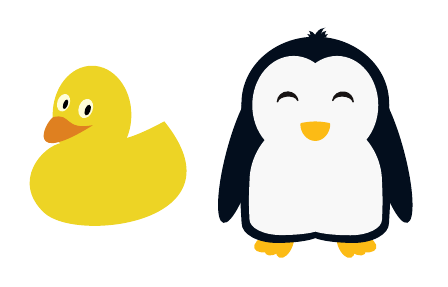
\begin{tikzpicture}
	\duck
	\pingu[xshift=2.8cm, yshift=14mm,
	       eyes wink]
\end{tikzpicture}
\end{tcblisting}

\subsection{Using the Coordinates}
\label{mrk:coordinates}While there are a lot of gadgets available already,
every penguin is accompanied by \textit{several} adaptive coordinates
to place custom items, texts,~\ldots\ % TODO: links
They can be visualized by the \keyref{meta-dots} option.
Furthermore, some extras create further coordinates themselves!
All coordinates are available with |<pingu-name>-<coordinate>|.
While the default name of a penguin is \say{pingu}, it can be
changed with the name option:
\begin{tcblisting}{title={Lotta dots},externalize listing=dotted-pengu}
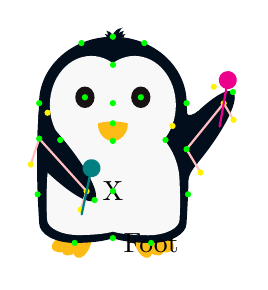
\begin{tikzpicture}
	\pingu[meta dots,left wing wave,
	       right wing grab, name=paula]
	\node at (paula-belly-center) {X};
	\node at (paula-foot-left) {Foot};
\end{tikzpicture}
\end{tcblisting}
Lets look at those coordinates in more detail (all labels are to be prefixed by |<pingu-name>-|):
\newsavebox\pinguwingright
\savebox\pinguwingright{%
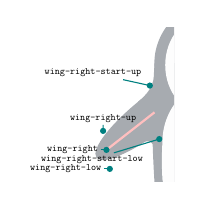
\begin{tikzpicture}%
	\scope
	\path[clip] (.25,-1.25) rectangle (-1.1,.7);
	\pgfonlayer{foreground}\path[clip] (.25,-1.25) rectangle (-1.1,.7);\endpgfonlayer
	\pingu[@block/.append style={fill=#1!35!white},wings hug,eyes shiny,heart=gray!30!white,feet=none]
	\path[draw,pink,thick] (pingu-wing-right-start) -- (pingu-wing-right);
	\endscope
	\foreach \c/\a/\n in {wing-right/left/.75mm,wing-right-low/left/.75mm,wing-right-up/above/.75mm,wing-right-start-low/below left/1.75mm,wing-right-start-up/above left/.75mm} {
		\path[fill=teal] (pingu-\c) circle [radius=1.125pt];
		\node[\a=\n,font=\ttfamily,scale=.35,inner sep=2.5pt] (expl-\c) at (pingu-\c) {\c};
		\draw[teal,thin] (expl-\c) -- (pingu-\c);
	}
\end{tikzpicture}}
\makeatletter
\newsavebox\pinguwingleft
\savebox\pinguwingleft{%
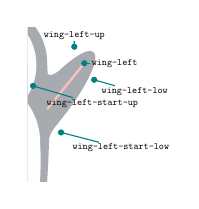
\begin{tikzpicture}%
	\scope
	\path[clip] (\pingu@w@half*2-.25cm,-1.25) rectangle ++(1.25,1.95);
	\pgfonlayer{foreground}\path[clip] (\pingu@w@half*2-.25cm,-1.25) rectangle ++(1.25,1.95);\endpgfonlayer
	\pingu[@block/.append style={fill=#1!35!white}, wings wave,eyes shiny,heart=gray!30!white,feet=none]
	\path[draw,pink,thick] (pingu-wing-left-start) -- (pingu-wing-left);
	\endscope
	\foreach \c/\a/\n in {wing-left/right/.75mm,wing-left-low/below right/.75mm,wing-left-up/above/.75mm,wing-left-start-low/below right/1.25mm,wing-left-start-up/below right/1.5mm} {
		\path[fill=teal] (pingu-\c) circle [radius=1.125pt];
		\node[\a=\n,font=\ttfamily,scale=.35,inner sep=1.5pt] (expl-\c) at (pingu-\c) {\c};
		\draw[teal,thin] (expl-\c) -- (pingu-\c);
	}
\end{tikzpicture}%
}
\vfill
\def\PinguCoords#1{\begin{tikzpicture}
	\pingu[@block/.append style={fill=##1!35!white}, wings wave,eyes shiny,heart=gray!30!white,#1]
	\pgfonlayer{foreground}
	\foreach \c/\a in {belly-center/above,head/below,head-top/above,foot-left/right,foot-right/left,eye-right/above left,eye-left/above right,bill/right,bill-bottom/below,wings-side-left/right,wings-side-right/left,wing-left-start/below right,wing-left-tip/right,wing-right-start/below left,wing-right-tip/left,head-right/left,head-left/right,head-center/below,head-back-con-left/above right,head-back-con-right/above left,bottom-center/above,waist-left/right,waist-right/left} {
		\path[fill=green] (pingu-\c) circle [radius=1.125pt];
		\node[\a=.5mm,font=\ttfamily,scale=.35,inner sep=1.5pt] (expl-\c) at (pingu-\c) {\c};
		\draw[green,thin] (expl-\c) -- (pingu-\c);
	}
	\endpgfonlayer
\end{tikzpicture}}%
\begin{center}
	\edef\measurepage{\the\dimexpr\pagegoal-\pagetotal-2\baselineskip\relax}%
	\ifdim\measurepage<4\baselineskip\clearpage\edef\measurepage{\the\dimexpr\pagegoal-\pagetotal-2\baselineskip\relax}\fi
	\resizebox*!{\measurepage}{%
		\PinguCoords{}%
	}
\end{center}

\paragraph{The Wings}
This view excluded a lot of special data collected on the wings!
While there is more information stored for each wing, the following five coordinates are the most important to place items into penguins hand:\vspace*{-1.5em}
\begin{center}
	\null\hfill\parbox[c]{2.5\wd\pinguwingright}{\scalebox{2.5}{\usebox\pinguwingright}}\hfill\parbox[c]{4cm}{\centering\small\@declaredcolor{gray}\sffamily And yes, the wings are deliberately placed asymmetrical.\endgraf}\hfill
	\parbox[c]{2.5\wd\pinguwingleft}{\scalebox{2.5}{\usebox\pinguwingleft}}\hfill\null
\end{center}

\paragraph{The Body} Similarly to the wing position, different
body types can change the coordinates (left the \keyref{body type} \textit{chubby} and right the \keyref{body type} \textit{legacy}):
\begin{center}
	\resizebox\linewidth!{%
		\PinguCoords{body type=chubby,wings hug}\quad\PinguCoords{body type=legacy,wings hug}
	}
\end{center}

\subsection{Colors}
A lot of options allow for a color to be passed. In general, you can provide any color that \TikZ\ is happy with! Yet, there are some predefined pingu-colors shipped with this package:
\def\getCol#1{\pgfmathparse{int(round(#1*255))}\pgfmathresult}
\def\parseRGB#1,#2,#3;{r:~\getCol{#1}, g:~\getCol{#2}, b:~\getCol{#3}}
\begin{multicols}{4}
\begin{itemize}
	\foreach \col in {main,black,silver,bronze,white,yellow,lightblue,blue,green,red,purple} {
		\item[{\tikz[baseline=-.6ex]{\fill[pingu@\col,semithick,draw=black] circle (4pt);}}] \footnotesize\strut
		% somehow outputs, therefore box
		\setbox0=\hbox{\colorInfoRGB{pingu@\col}\xdef\colorValue{\colorValue}}\rlap{\smash{\raisebox{-2.9mm}{\sffamily\color{gray}\tiny\expandafter\parseRGB\colorValue;}}}%
		\texttt{pingu@\col}%
	}
	\item[] \footnotesize\strut% buffer
\end{itemize}
\end{multicols}
Furthermore, there is the special color {\makeatletter\say{\expandafter\ipingu\expandafter{\@pingu@none}}} which is available for most\footnote{Why just \say{most}? Well, this package is work in progress and I have added the option late, so I may have forgotten to patch some keys.} extras and wing-items. This color prohibits the compartments from being drawn. To be more precise, the package defines the macro \ltex{\\@pingu@none}, which is matched against the selected color.

As an example, lets take a look at the \keyref{cup}-extra, which provides an additional key \keyref{cup straw} to color the straw:
\begin{tcblisting}{title={Cup without a straw},externalize listing=extra-options}
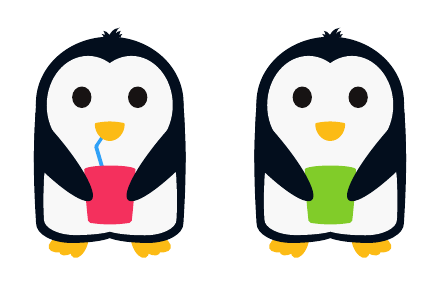
\begin{tikzpicture}
	\pingu[wings grab, cup=pingu@purple,
	       cup straw=pingu@blue]
	\pingu[wings grab, cup, xshift=2.8cm,
	       cup straw=!hide]
\end{tikzpicture}
\end{tcblisting}
As you can see, using \lpingu{!hide}, the straw will not be drawn.

\subsection{Setting the defaults}
You do not have to re-state every key.
With \lstinline[language=pingulang]'\pingudefaults' and \lstinline[language=pingulang]'\pingudefaultsappend' (similar, but extends the current options) you can set default-options for all penguins to come:
\begin{tcblisting}{title={Change the mainstream},externalize listing=update-defaults}
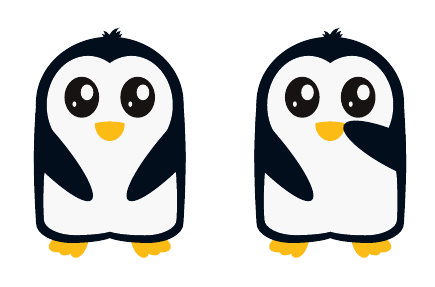
\begin{tikzpicture}
	\pingudefaults{wings grab, eyes shiny}
	\pingu
	\pingu[left wing shock, xshift=2.8cm]
\end{tikzpicture}
\end{tcblisting}

\subsection{Libraries}
\label{Libraries}\index{Libraries}I've split the penguin features into a set of libraries. While all of them are loaded by default, the |bare| package-option disables the automatic loading of all libraries. They can be loaded (locally to the current group) using |\pinguloadlibrary| and |\pinguloadlibraries| passing on a comma separated list of desired libraries.
See the full reference or the index to learn which key comes from which library.
Please note that~--- at the moment~--- not all components of a library are labeled correctly.
% TODO: already count that? % global let?
\foreach[count=\i] \l/\xs in \pingu@defaultlibs{\xdef\pingu@defaultlibs@count{\i}}%
Currently there are the following libraries:
\foreach[count=\i] \l/\xs in \pingu@defaultlibs{%
	\ifx\l\empty\else
	\index{Libraries!\textit{\l}}\textit{\l}\ifnum\numexpr\pingu@defaultlibs@count-1>\i,\space\else
	\ifnum\pingu@defaultlibs@count=\i\else,~and\space\fi\fi
	\fi
}.

\subsection{Changing the wings}
\label{subsec:wings}As already demonstrated, it is possible to change the wing positions!
All selected wing-items will adapt to the wing-position (although not all wing-items will make sense with every wing-position).
Currently, there are the following wing-positions:
\typesetselection{leftwing}. \say{none} is a special wing-position: it omits the drawing of wings (teaser: every selection has a none-option, which prohibits the part from being drawn)!

For each valid wing-position you can use |wings <position>| to change both wings or |left wing <position>| and |right wing <position>| to change only one wing respectively. The default wing-position is \say{normal}. If you supply multiple options for a wing, only the last one survives.\footnote{For the sake of completeness: \ipingu{wings <position>}, \ipingu{left wing <position>}, and \ipingu{right wing <position>} are just alternatives i prefer: \ipingu{wings=<position>}, \ipingu{left wing=<position>} and \ipingu{right wing=<position>}.}
This is shown in Box~\say{\nameref{wing-showcase}}.

\begin{tcblisting}{sidebyside=false, title=Wing-Showcase,nameref=Wing-Showcase,externalize listing=wings-showcase,float,phantomlabel=wing-showcase}
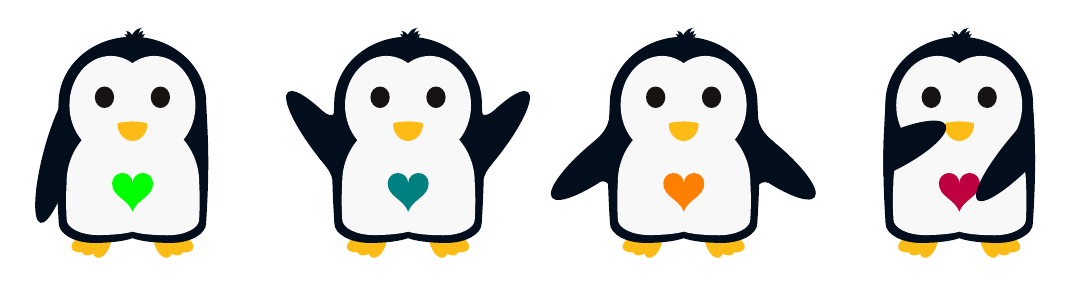
\begin{tikzpicture}
	\pingu[left wing none, heart=green]
	\pingu[wings wave, heart=teal, xshift=3.5cm]
	\pingu[wings hug, heart=orange, xshift=7cm]
	\pingu[left wing grab, right wing shock, heart=purple,  xshift=10.5cm]
\end{tikzpicture}
\end{tcblisting}

\subsection{Changing the eyes}
\label{mrk:pengu-eye}Just like the wings, there are a couple of different eye-styles to choose from: \typesetselection{lefteye}.
Similar to the wings, there is a \say{none} and a \say{normal}-option (which is the default).
Furthermore, the convenient selectors |eyes <style>|, |left eye <style>|, and |right eye <style>| exist as well. All of this is showcased in~Box~\say{\nameref{eye-showcase}}.

\begin{tcblisting}{sidebyside=false,title=Eye-Showcase,nameref=Eye-Showcase,externalize listing=eyes-showcase,float,phantomlabel=eye-showcase}
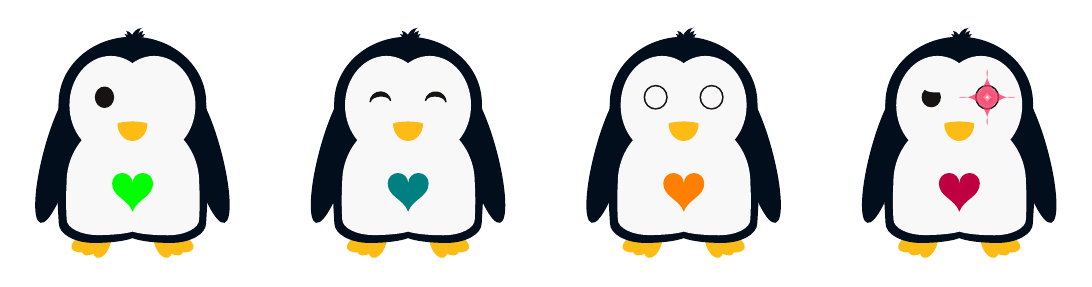
\begin{tikzpicture}
	\pingu[left eye none, heart=green]
	\pingu[eyes wink, heart=teal, xshift=3.5cm]
	\pingu[eyes shock, heart=orange, xshift=7cm]
	\pingu[left eye devil, right eye angry, heart=purple,  xshift=10.5cm]
\end{tikzpicture}
\end{tcblisting}

\subsection{Changing other components}
\label{mrk:pengu-change-comps}Just like for the wings and the eyes, you can change the following body parts:
\begin{itemize}
	\itemsep0pt\relax
	\item The \textit{body type} itself\\*
		Select from: \typesetselection{bodytype}.
	\item The \textit{feet} (again with separate left and right)\\*
		Select from: \typesetselection{leftfoot}.
	\item The \textit{bill} (does not have left and right, as there is just one)\\*
		Select from: \typesetselection{bill}.
	\item The \textit{hairstyle} (does not have left and right)\\*
		Select from: \typesetselection{hairstyle}.
\end{itemize}
For each selection, \say{none} will prohibit the drawing, and \say{normal} is the default chosen. See Box~\say{\nameref{bodyparts-showcase}} for a example.
\begin{tcblisting}{sidebyside=false,title=Bodyparts-Showcase,nameref=Bodyparts-Showcase,externalize listing=bodyparts-showcase,float,phantomlabel=bodyparts-showcase}

\begin{tikzpicture}
	\pingu[bill angry, heart=green]
	\pingu[feet back, hairstyle none, heart=teal, xshift=3.5cm]
	\pingu[bill flat, feet simple, heart=orange, xshift=7cm]
	\pingu[feet none, bill none, heart=purple, xshift=10.5cm]
\end{tikzpicture}
\end{tcblisting}

\subsection{Predefined Styles}
While the penguin options offer the modification of basically every drawing routine (through other styles like |@block|), it is tedious to change them every time.
So I have started to create some predefined styles, that do change some of the penguins appearance (and are completely new, so beware of bugs):
\begin{multicols}{2}
\begin{itemize}
	\itemsep0pt
	\foreach \tx/\s in {{draw everything with a line}/{:line}, {fill main penguin}/{:fill}, {draw components with transparency}/{:ghost parts}, {draw all layers with transparency}/{:ghost}, {set main \say{devil}-components}/{:devil},{flip the penguin (swaps left \& right)}/{:back},{do not draw main pingu}/{:hide}} {
		\item \parbox[t]{.8\linewidth}{\raggedright\texttt{\s}, \tx.} \hfill
		\parbox[t]{.175\linewidth}{\scalebox{.4}{%
			
\begin{tikzpicture}[baseline=.35\baselineskip]%
				\pingu[\s]
			\end{tikzpicture}%
		}}
	}
	\item[] \parbox[t][2.25\baselineskip]{0pt}{}% buffer
\end{itemize}
\end{multicols}
Currently, only some of the styles do affect other items. As an example, consider |:line|, that changes the draw-style of wing-items and extras:
\begin{tcblisting}{title={Line Penguin},externalize listing=line-pengu}
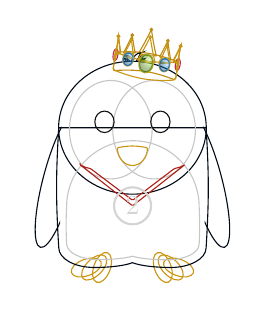
\begin{tikzpicture}
	\pingu[:line, princess crown, silver medal]
\end{tikzpicture}
\end{tcblisting}

\subsection{Randomness}
Each selection (like the wings or the eyes) can receive a special command \lpingu{!random}. If given, the penguin will receive a randomly picked component.
Please note, that \textit{none} (the component removing it) will never be picked.
The first line in the example in Box~\say{\nameref{random-penguin}} sets the seed. % we do not externalize this one
\begin{tcblisting}{title={Random Penguin},nameref={Random Penguin},label=random-penguin,float}
\pgfmathsetseed{\number\pdfrandomseed}

\begin{tikzpicture}
	\pingu[wings=!random,eyes=!random,
		   body type=!random,
			left foot=!random,
			bill=!random,
			hairstyle=!random]
\end{tikzpicture}
\end{tcblisting}

In a more general fashion, there is a \keyref{random from} key for completely random penguins.

\keyexplain{random from}{list}{}
	You can pass any list of penguin keys and exactly one of them will be selected. You can nest \keyref{random from}-calls. Please note, that the items are not separated by comma but in braces. The first line in the example sets the seed:% do not externalize
\begin{tcblisting}{}
\pgfmathsetseed{\number\pdfrandomseed}

\begin{tikzpicture}
	\pingu[random from={{eye patch left}{eye patch right}{halo,halo raise=4mm}},random from={{right eye color=pingu@blue}{random from={{bow tie}{gold medal}}}},random from={{eyes=!random}{wings=!random}},body type=legacy]
\end{tikzpicture}
\end{tcblisting}
\endkeyexplain


\subsection{Extras}
An extra is considered everything, that is attached to the main penguin and not to the wings (as those items may be placed separately for both wings).
Most extras are activated with the format |<extra>=<color>| (the |<color>| option is not mandatory)
and try to adapt with other extras that have been placed (yet you can place multiple hats if you really like to).  A lot of the extras do offer more keys to customize their appearance.
They are explained in the full reference (\autoref{sec:full-ref}).

Consider the somewhat overkill-example of \say{\nameref{lord-gadget}}.
\begin{tcblisting}{title={Lord-Gadget, the penguin},externalize listing=lord-gadget,nameref={Lord-Gadget, the penguin},label=lord-gadget,float}

\begin{tikzpicture}
	\pingu[crown 2d=pingu@bronze,
	       medal=pingu@purple, tie,
	       eye patch left=teal,
	       eye patch right=orange,
	       right wing wave, sunglasses,
	       glow thick=yellow]
\end{tikzpicture}
\end{tcblisting}

\subsection{Wing-Items}
Wing items are basically just like extras, but they can be selected separately for the left and right wing. Furthermore, they adapt their \textit{default} appearance to the active wing positions (\autoref{subsec:wings}).
Currently there are the following wing items:
% add a extra guard not present with the wing items
\typesetselection[\textit{#1\expandafter\ParseDTLListElement :"#1"\@nil}]{wingitems}.
They are selected using |<wing item> <left/right>|.

Additionally, they can be customized by \keyref{left item angle} and \keyref{right item angle}, as well as \keyref{left item flip} and \keyref{right item flip}.
Lets consider an example\ldots
\begin{tcblisting}{title={Penguin with full wings!}}

\begin{tikzpicture}[scale=.75]
	\pingu[lightsaber right=orange,
	  lollipop left,
	  right item angle=70,
	  right wing raise, left wing grab]
	\pingu[cane left, right item flip,
	  sign post right={Hi!}, xshift=35mm]
\end{tikzpicture}
\end{tcblisting}

\subsection{Clothing}
Clothing is the newest extension to the collection, at and the moment there is not one \say{real} clothing, that really adapts to the penguins-position.
I am working on the \textit{cloak}-Clothing at the moment:
\begin{tcblisting}{title={Pengu-Clothes},externalize listing=clothes}

\begin{tikzpicture}[scale=.75]
	\pingu[cloak]
\end{tikzpicture}
\end{tcblisting}

% \section{Examples}

\appendix
\section{Gadget Overview}\label{Gadget-Overview}

\TypesetShowcases

\section{Full Reference}\label{sec:full-ref}

\def\percenttargetreductionpengus{63}\def\lstfnsize{-1.65}
\tcbset{%
	before lower={\begin{adjustbox}{scale=.\percenttargetreductionpengus}},
	after lower={\end{adjustbox}},%
	boxsep=1pt%
}

\begin{center}
	\textit{Please note, that all preview-penguins have been reduced in scale to \percenttargetreductionpengus\,\% to save space and make the documentation more concise.}
\end{center}

Aliases may set custom defaults. Those defaults are not listed as they may change.

\subsection{Penguin Keys}

\keyexplain{name}{text}{\pingu@name}
	Sets the name of the penguin. This name is used for all the automatically generated coordinates (see~\autoref{mrk:coordinates}).
\endkeyexplain

\keyexplain{scale}{floating point}{active scale}
	Changes the scale for the penguin. This is not supported by all items by default (as some scales have to be re-calculated according to their rotation).
	Yet, it should work with most.

	Furthermore, this value can be used to make the penguin independent of the outer scaling.
\endkeyexplain


\keyexplain{meta-dots}{true/false}{\if@pingu@draw@metadots true\else false\fi}
	Can be used to enable and disable the meta dots (\autoref{mrk:coordinates}).
	Passed true by default.
\endkeyexplain

\keyalias{meta dots}{meta-dots}

\subsubsection{The Feet}

\keyexplain{left foot}{foot-selector}{\@pingu@select@leftfoot@}
	Change the style of the left foot. All valid values are listed in \autoref{mrk:pengu-change-comps}.
\begin{tcblisting}{listing options={style=lstpingu,language=pingulang,deleteemph={[2]{simple}}}}

\begin{tikzpicture}
	\pingu[left foot=simple]
\end{tikzpicture}
\end{tcblisting}
\endkeyexplain


\keyexplain{left foot color}{color}{\pingu@color@foot@left}
\begin{tcblisting}{@}
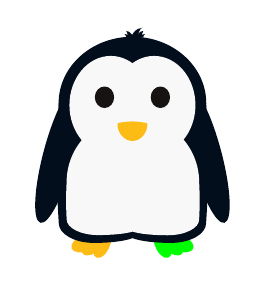
\begin{tikzpicture}
	\pingu[left foot color=green]
\end{tikzpicture}
\end{tcblisting}
\endkeyexplain

\shortcuts{left foot}{\@pingu@leftfoot@}{left foot color}

\keyexplain{right foot}{foot-selector}{\@pingu@select@rightfoot@}
	Change the style of the right foot. All valid values are listed in \autoref{mrk:pengu-change-comps}.
\begin{tcblisting}{listing options={style=lstpingu,language=pingulang,deleteemph={[2]{simple}}}}

\begin{tikzpicture}
	\pingu[right foot=simple]
\end{tikzpicture}
\end{tcblisting}
\endkeyexplain


\keyexplain{right foot color}{color}{\pingu@color@foot@right}
\begin{tcblisting}{@}
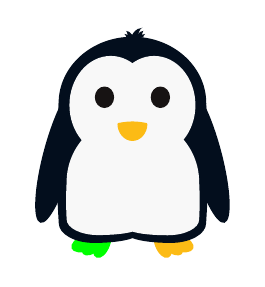
\begin{tikzpicture}
	\pingu[right foot color=green]
\end{tikzpicture}
\end{tcblisting}
\endkeyexplain

\shortcuts{right foot}{\@pingu@rightfoot@}{right foot color}

\keyexplain{feet}{foot-selector}{}
	Change the style of both feet by calling \keyref{left foot} and \keyref{right foot} with the same value.
\begin{tcblisting}{listing options={style=lstpingu,language=pingulang,deleteemph={[2]{simple}}}}

\begin{tikzpicture}
	\pingu[feet=simple]
\end{tikzpicture}
\end{tcblisting}
\endkeyexplain


\keyexplain{feet color}{color}{}
	Sets the color of both feet (using \keyref{left foot color} and \keyref{right foot color}).
\begin{tcblisting}{@}
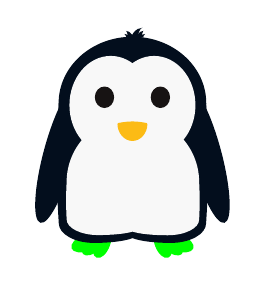
\begin{tikzpicture}
	\pingu[feet color=green]
\end{tikzpicture}
\end{tcblisting}
\endkeyexplain

\shortcuts{feet}{\@pingu@leftfoot@}{feet color}

\subsubsection{The Body}

\keyexplain{body main}{color}{\pingu@color@body@main}
	Set the main color of the penguin. This will affect \keyref{hair} as well, as this chooses its default value from the main color.%
\begin{tcblisting}{@}
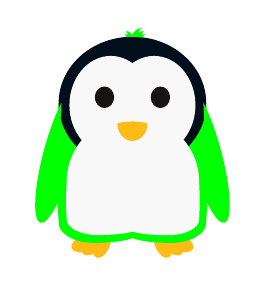
\begin{tikzpicture}
	\pingu[body main=green]
\end{tikzpicture}
\end{tcblisting}
\endkeyexplain


\keyexplain{body head}{color}{\pingu@color@body@head}
	Set the color of the penguin head.%
\begin{tcblisting}{@}
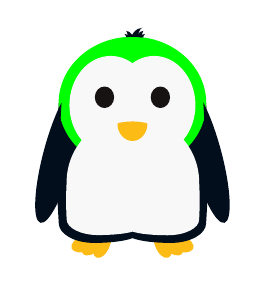
\begin{tikzpicture}
	\pingu[body head=green]
\end{tikzpicture}
\end{tcblisting}
\endkeyexplain


\keyexplain{body}{color}{}
	Sets the color of the main penguin and the head, by calling \keyref{body main} and \keyref{body head} with the same value.
\begin{tcblisting}{@}

\begin{tikzpicture}
	\pingu[body=green]
\end{tikzpicture}
\end{tcblisting}
\endkeyexplain


\keyexplain{body front}{color}{\pingu@color@body@front}
	Sets the frontal color of the penguin.
\begin{tcblisting}{@}
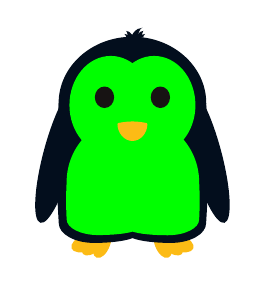
\begin{tikzpicture}
	\pingu[body front=green]
\end{tikzpicture}
\end{tcblisting}
\endkeyexplain


\keyexplain{body type}{body type}{normal}
	Change the active body type. All valid values are listed in \autoref{mrk:pengu-change-comps}:
\begin{tcblisting}{@}

\begin{tikzpicture}
	\pingu[body type=legacy]
\end{tikzpicture}
\end{tcblisting}
\endkeyexplain

\subsubsection{The Size}


\keyexplain{height}{length}{\the\pingu@side@h@half}
	Change the height of the penguin manually. You probably should not use this key directly and refer to \keyref{small size}, \keyref{normal size}, and \keyref{large size}:
\begin{tcblisting}{listing options={style=lstpingu,language=pingulang}}

\begin{tikzpicture}
	\pingu[height=17mm]
\end{tikzpicture}
\end{tcblisting}
\endkeyexplain


\keyexplain{small size}{}{}
	Will use \keyref{height} to create a small pingu:
\begin{tcblisting}{listing options={style=lstpingu,language=pingulang}}

\begin{tikzpicture}
	\pingu[small size]
\end{tikzpicture}
\end{tcblisting}
\endkeyexplain

\keyalias{small}{small size}
\keyalias{small height}{small size}


\keyexplain{normal size}{}{}
	Will use \keyref{height} to create a normal pingu:
\begin{tcblisting}{listing options={style=lstpingu,language=pingulang}}

\begin{tikzpicture}
	\pingu[normal size]
\end{tikzpicture}
\end{tcblisting}
\endkeyexplain

\keyalias{normal}{normal size}
\keyalias{normal height}{normal size}


\keyexplain{large size}{}{}
	Will use \keyref{height} to create a large pingu:
\begin{tcblisting}{listing options={style=lstpingu,language=pingulang}}

\begin{tikzpicture}
	\pingu[large size]
\end{tikzpicture}
\end{tcblisting}
\endkeyexplain

\keyalias{large}{large size}
\keyalias{large height}{large size}

\subsubsection{The Eyes}
\keyexplain{left eye}{eye-selector}{\@pingu@select@lefteye@}
	Change the style of the left eye. All valid values are listed in \autoref{mrk:pengu-eye}.
\begin{tcblisting}{listing options={style=lstpingu,language=pingulang,deleteemph={[2]{wink}}}}

\begin{tikzpicture}
	\pingu[left eye=wink]
\end{tikzpicture}
\end{tcblisting}
\endkeyexplain


\keyexplain{left eye color}{color}{\pingu@color@eye@left}
\begin{tcblisting}{@}
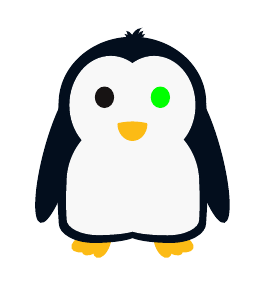
\begin{tikzpicture}
	\pingu[left eye color=green]
\end{tikzpicture}
\end{tcblisting}
\endkeyexplain


\keyexplain{left eye second color}{color}{\pingu@color@eye@second@left}
	Change the secondary color of the left eye. It will be used in some styles selected by \keyref{left eye} (e.g. \textit{shiny}):
\begin{tcblisting}{listing options={style=lstpingu,language=pingulang,deleteemph={[2]{shiny}}}}
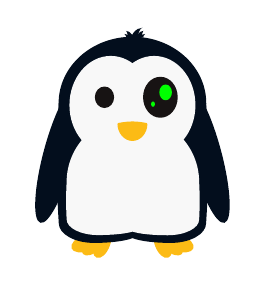
\begin{tikzpicture}
	\pingu[left eye=shiny,
	  left eye second color=green]
\end{tikzpicture}
\end{tcblisting}
\endkeyexplain

\shortcuts{left eye}{\@pingu@lefteye@}{left eye color}

\keyexplain{right eye}{eye-selector}{\@pingu@select@righteye@}
	Change the style of the right eye. All valid values are listed in \autoref{mrk:pengu-eye}.
\begin{tcblisting}{listing options={style=lstpingu,language=pingulang,deleteemph={[2]{wink}}}}

\begin{tikzpicture}
	\pingu[right eye=wink]
\end{tikzpicture}
\end{tcblisting}
\endkeyexplain


\keyexplain{right eye color}{color}{\pingu@color@eye@right}
\begin{tcblisting}{@}
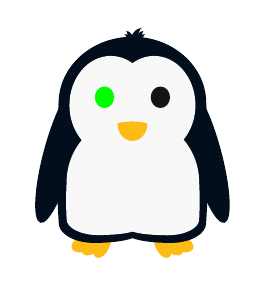
\begin{tikzpicture}
	\pingu[right eye color=green]
\end{tikzpicture}
\end{tcblisting}
\endkeyexplain


\keyexplain{right eye second color}{color}{\pingu@color@eye@second@right}
	Change the secondary color of the right eye. It will be used in some styles selected by \keyref{right eye} (e.g. \textit{shiny}):
\begin{tcblisting}{listing options={style=lstpingu,language=pingulang,deleteemph={[2]{shock}}}}
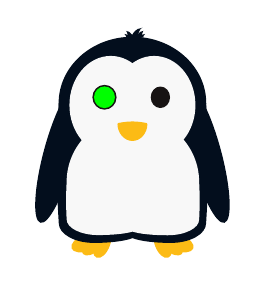
\begin{tikzpicture}
	\pingu[right eye=shock,
	  right eye second color=green]
\end{tikzpicture}
\end{tcblisting}
\endkeyexplain

\shortcuts{right eye}{\@pingu@righteye@}{right eye color}

\keyexplain{eyes}{eye-selector}{}
	Change the style of both eyes by calling \keyref{left eye} and \keyref{right eye} with the same value.
\begin{tcblisting}{listing options={style=lstpingu,language=pingulang,deleteemph={[2]{wink}}}}

\begin{tikzpicture}
	\pingu[eyes=wink]
\end{tikzpicture}
\end{tcblisting}
\endkeyexplain


\keyexplain{eyes color}{color}{}
	Change the main color of both eyes by calling \keyref{left eye color} and \keyref{right eye color} with the same value.
\begin{tcblisting}{@}
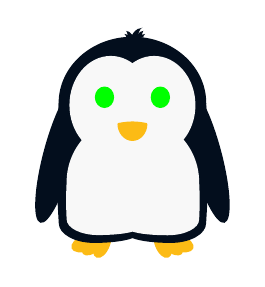
\begin{tikzpicture}
	\pingu[eyes color=green]
\end{tikzpicture}
\end{tcblisting}
\endkeyexplain


\keyexplain{eyes second color}{color}{}
	Change the secondary color of  both eyes by calling \keyref{left eye second color} and \keyref{right eye second  color} with the same value.
\begin{tcblisting}{listing options={style=lstpingu,language=pingulang,deleteemph={[2]{shock,shiny}}}}
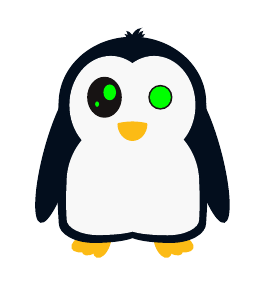
\begin{tikzpicture}
	\pingu[left eye=shock, right eye=shiny,
	  eyes second color=green]
\end{tikzpicture}
\end{tcblisting}
\endkeyexplain

\shortcuts{eyes}{\@pingu@lefteye@}{eyes color}

\subsubsection{The Wings}

\keyexplain{left wing}{wing-selector}{\@pingu@select@leftwing@}
	Change the style of the left wing. All valid values are listed in \autoref{subsec:wings}.
\begin{tcblisting}{listing options={style=lstpingu,language=pingulang,deleteemph={[2]{wave}}}}

\begin{tikzpicture}
	\pingu[left wing=wave]
\end{tikzpicture}
\end{tcblisting}
\endkeyexplain

\keyexplain{left wing color}{color}{\pingu@color@left@wing}
\begin{tcblisting}{@}

\begin{tikzpicture}
	\pingu[left wing color=green]
\end{tikzpicture}
\end{tcblisting}
\endkeyexplain

\shortcuts{left wing}{\@pingu@leftwing@}{left wing color}

\keyexplain{right wing}{wing-selector}{\@pingu@select@rightwing@}
	Change the style of the right wing. All valid values are listed in \autoref{subsec:wings}.
\begin{tcblisting}{listing options={style=lstpingu,language=pingulang,deleteemph={[2]{wave}}}}

\begin{tikzpicture}
	\pingu[right wing=hug]
\end{tikzpicture}
\end{tcblisting}
\endkeyexplain

\keyexplain{right wing color}{color}{\pingu@color@right@wing}
\begin{tcblisting}{@}
\begin{tikzpicture}
	\pingu[right wing color=green]
\end{tikzpicture}
\end{tcblisting}
\endkeyexplain

\shortcuts{right wing}{\@pingu@rightwing@}{right wing color}

\keyexplain{wings}{wing-selector}{}
	Change the style of both wings by calling \keyref{left wing} and \keyref{right wing} with the same value.
\begin{tcblisting}{listing options={style=lstpingu,language=pingulang,deleteemph={[2]{wink}}}}
\begin{tikzpicture}
	\pingu[wings=grab]
\end{tikzpicture}
\end{tcblisting}
\endkeyexplain

\keyexplain{wings color}{color}{}
	Change the main color of both wings by calling \keyref{left wing color} and \keyref{right wing color} with the same value.
\begin{tcblisting}{@}
\begin{tikzpicture}
	\pingu[wings color=green]
\end{tikzpicture}
\end{tcblisting}
\endkeyexplain

\shortcuts{wings}{\@pingu@leftwing@}{wings color}

\subsubsection{The Hair}


\keyexplain{hair 1 color}{color}{\pingu@color@hair@a}
	Set the color of the first hair (this may be used differently by other hairstyles):
\begin{tcblisting}{listing options={style=lstpingu,language=pingulang,moreemph={[2]{1}}}}
\begin{tikzpicture}
	\pingu[hair 1 color=green]
\end{tikzpicture}
\end{tcblisting}
\endkeyexplain

\keyexplain{hair 2 color}{color}{\pingu@color@hair@b}
	Set the color of the second hair (this may be used differently by other hairstyles):
\begin{tcblisting}{listing options={style=lstpingu,language=pingulang,moreemph={[2]{2}}}}
\begin{tikzpicture}
	\pingu[hair 2 color=green]
\end{tikzpicture}
\end{tcblisting}
\endkeyexplain

\keyexplain{hair 3 color}{color}{\pingu@color@hair@c}
	Set the color of the third hair (this may be used differently by other hairstyles):
\begin{tcblisting}{listing options={style=lstpingu,language=pingulang,moreemph={[2]{3}}}}
\begin{tikzpicture}
	\pingu[hair 3 color=green]
\end{tikzpicture}
\end{tcblisting}
\endkeyexplain

\keyexplain{hair 4 color}{color}{\pingu@color@hair@d}
	Set the color of the fourth hair (this may be used differently by other hairstyles):
\begin{tcblisting}{listing options={style=lstpingu,language=pingulang,moreemph={[2]{4}}}}
\begin{tikzpicture}
	\pingu[hair 4 color=green]
\end{tikzpicture}
\end{tcblisting}
\endkeyexplain

\keyexplain{hair 5 color}{color}{\pingu@color@hair@e}
	Set the color of the fifth hair (this may be used differently by other hairstyles):
\begin{tcblisting}{listing options={style=lstpingu,language=pingulang,moreemph={[2]{5}}}}
\begin{tikzpicture}
	\pingu[hair 5 color=green]
\end{tikzpicture}
\end{tcblisting}
\endkeyexplain

\keyexplain{hairs color}{color}{}
	Set the color of all hairs by calling \keyref{hair 1 color}, \keyref{hair 2 color}, \keyref{hair 3 color}, \keyref{hair 4 color}, and \keyref{hair 5 color} with the same argument:
\begin{tcblisting}{@}
\begin{tikzpicture}
	\pingu[hairs color=green]
\end{tikzpicture}
\end{tcblisting}
\endkeyexplain

\keyalias{hairs}{hairs color}
\keyalias{hair}{hairs color}

\keyexplain{hairstyle}{hair-selector}{\@pingu@select@hairstyle@}
	Change the hairstyle (\autoref{mrk:pengu-change-comps}):
\begin{tcblisting}{@}
\begin{tikzpicture}
	\pingu[hairstyle=none]
\end{tikzpicture}
\end{tcblisting}
\endkeyexplain

\keyalias{hair style}{hairstyle}
\shortcuts{hairstyle}{\@pingu@hairstyle@}{hairs color}

\subsubsection{The Bill}
\keyexplain{bill}{bill-selector}{\@pingu@select@bill@}
	Change the style of the bill (\autoref{mrk:pengu-change-comps}):
\begin{tcblisting}{listing options={style=lstpingu,language=pingulang,deleteemph={[2]{flat}}}}
\begin{tikzpicture}
	\pingu[bill=flat]
\end{tikzpicture}
\end{tcblisting}
\endkeyexplain

\keyexplain{bill color}{color}{\pingu@color@bill}
\begin{tcblisting}{@}
\begin{tikzpicture}
	\pingu[bill color=green]
\end{tikzpicture}
\end{tcblisting}
\endkeyexplain

\shortcuts{bill}{\@pingu@bill@}{bill color}

\subsection{Drawing Styles}
\index{Styles}
\def\cursub{Styles!}
\keyexplain{:line}{}{}
	Disable glows, shades and fills and enforce a line. This line will be darker
	than the original fill color:
\begin{tcblisting}{@}
\begin{tikzpicture}
	\pingu[:line]
\end{tikzpicture}
\end{tcblisting}
\endkeyexplain

\keyexplain{:fill}{}{}
	Makes the whole penguin in one solid color (basically a shortcut for setting all main penguin colors to the same):
\begin{tcblisting}{@}
\begin{tikzpicture}
	\pingu[:fill]
\end{tikzpicture}
\end{tcblisting}
\endkeyexplain

\keyexplain{:ghost parts}{opacity}{.5}
	Set the opacity of each penguin component individually. At the moment, this
	excludes some glow calculations.
\begin{tcblisting}{@}
\begin{tikzpicture}
	\pingu[:ghost parts]
\end{tikzpicture}
\end{tcblisting}
\endkeyexplain

\keyexplain{:ghost}{opacity}{.5}
	Set the opacity of the complete penguin. At the moment, this
	excludes some glow calculations.
\begin{tcblisting}{@}
\begin{tikzpicture}
	\pingu[:ghost]
\end{tikzpicture}
\end{tcblisting}
\endkeyexplain

\keyexplain{:devil}{color}{pingu@purple}
	Enable all devil components (not the wing items) and set their main color:
\begin{tcblisting}{@}
\begin{tikzpicture}
	\pingu[:devil=green]
\end{tikzpicture}
\end{tcblisting}
\endkeyexplain


\keyexplain{:hide}{}{}
	Do not draw the main pingu:
\begin{tcblisting}{@}
\begin{tikzpicture}
	\pingu[santa hat,:hide]
\end{tikzpicture}
\end{tcblisting}
\endkeyexplain

\keyexplain{:back}{}{}
	Mirror the penguin, this swaps left and right, the rotation and more.
	Yet, at least at the time of writing, this does not swap the drawing order in each layer, but just the layers:
\begin{tcblisting}{@}
\begin{tikzpicture}
	\pingu[:back, left wing wave,
	       cane left, left item angle=70]
\end{tikzpicture}
\end{tcblisting}
\endkeyexplain

\def\cursub{}

\subsection{Extras}
\subsubsection{The heart}
\showkeyexplain{heart}{node-options}{}(pingu@main)
\begin{tcblisting}{@}
\begin{tikzpicture}
	\pingu[heart=green]
\end{tikzpicture}
\end{tcblisting}
\endshowkeyexplain

\subsubsection{The tie}
\showkeyexplain{tie}{color}{pingu@green}
\begin{tcblisting}{@}
\begin{tikzpicture}
	\pingu[tie]
\end{tikzpicture}
\end{tcblisting}
\endshowkeyexplain

{\def\pingu@color@tie{<tie-color>}
\subkeyexplain{tie}{tie knot}{color}{\pingu@color@tie@knot}
\begin{tcblisting}{@}
\begin{tikzpicture}
	\pingu[tie, tie knot=orange]
\end{tikzpicture}
\end{tcblisting}
\endsubkeyexplain
}

\subkeyexplain{tie}{tie length}{length}{\expandafter\detokenize\expandafter{\pingu@x@tie@length}}
\begin{tcblisting}{@}
\begin{tikzpicture}
	\pingu[tie, tie length=1.25cm]
\end{tikzpicture}
\end{tcblisting}
\endsubkeyexplain

\subkeyexplain{tie}{tie offset}{length}{\pingu@x@tie@offset}
	Change the upper vertical offset of the tie:
\begin{tcblisting}{@}
\begin{tikzpicture}
	\pingu[tie, tie offset=.75cm]
\end{tikzpicture}
\end{tcblisting}
\endsubkeyexplain

\subkeyexplain{tie}{tie width}{length}{\pingu@x@tie@width}
\begin{tcblisting}{@}
\begin{tikzpicture}
	\pingu[tie, tie width=.5cm]
\end{tikzpicture}
\end{tcblisting}
\endsubkeyexplain

\subkeyexplain{tie}{tie pattern}{tex-code}{}
	Change the tie pattern.
\endsubkeyexplain

\subkeyexplain{tie}{tie dots}{color}{pingu@white}
	Change the \keyref{tie pattern} to dots:
	\begin{tcblisting}{@}
	\begin{tikzpicture}
		\pingu[tie, tie dots]
	\end{tikzpicture}
	\end{tcblisting}
\endsubkeyexplain

\subsubsection{The bowtie}
\showkeyexplain{bow tie}{color}{pingu@blue}
\begin{tcblisting}{@}
\begin{tikzpicture}
	\pingu[bow tie]
\end{tikzpicture}
\end{tcblisting}
\endshowkeyexplain

\keyalias{bowtie}{bow tie}
\keyalias{bow-tie}{bow tie}

\subkeyexplain{bow tie}{bow tie b}{color}{<bowtie-color>}
\begin{tcblisting}{@}
\begin{tikzpicture}
	\pingu[bow tie, bow tie b=green]
\end{tikzpicture}
\end{tcblisting}
\endsubkeyexplain

\subkeyalias{bowtie b}{bow tie b}{bow tie}
\subkeyalias{bow-tie b}{bow tie b}{bow tie}

{\def\pingu@color@bowtie{<bowtie-color>}
\subkeyexplain{bow tie}{bow tie knot}{color}{\pingu@color@bowtie@knot}
\begin{tcblisting}{@}
\begin{tikzpicture}
	\pingu[bow tie, bow tie knot=green]
\end{tikzpicture}
\end{tcblisting}
\endsubkeyexplain

\subkeyalias{bowtie knot}{bow tie knot}{bow tie}
\subkeyalias{bow-tie knot}{bow tie knot}{bow tie}
}

\subkeyexplain{bow tie}{bow tie offset}{length}{\pingu@x@bowtie@offset}
\begin{tcblisting}{@}
\begin{tikzpicture}
	\pingu[bow tie, bow tie offset=8mm]
\end{tikzpicture}
\end{tcblisting}
\endsubkeyexplain

\subkeyalias{bowtie offset}{bow tie offset}{bow tie}
\subkeyalias{bow-tie offset}{bow tie offset}{bow tie}

\subsubsection{The cup}

\showkeyexplain{cup}{color}{pingu@green}
\begin{tcblisting}{@}
\begin{tikzpicture}
	\pingu[cup]
\end{tikzpicture}
\end{tcblisting}
\endshowkeyexplain

{\def\pingu@color@cup{<cup-color>}
\subkeyexplain{cup}{cup straw}{color}{\pingu@color@cup@straw}
\begin{tcblisting}{@}
\begin{tikzpicture}
	\pingu[cup, cup straw=!hide]
\end{tikzpicture}
\end{tcblisting}
\endsubkeyexplain}

\subsubsection{The medal}
\showkeyexplain{medal}{color}{pingu@yellow}
\begin{tcblisting}{@}
\begin{tikzpicture}
	\pingu[medal]
\end{tikzpicture}
\end{tcblisting}
\endshowkeyexplain

\subkeyexplain{medal}{medal band}{color}{\pingu@color@medal@band}
\begin{tcblisting}{@}
\begin{tikzpicture}
	\pingu[medal, medal band=green]
\end{tikzpicture}
\end{tcblisting}
\endsubkeyexplain

{\def\pingu@color@medal{<medal-color>}
\subkeyexplain{medal}{medal shade}{color}{\pingu@color@medal@shade}
Change the color of the outer medal ring:
\begin{tcblisting}{@}
\begin{tikzpicture}
	\pingu[medal, medal shade=green]
\end{tikzpicture}
\end{tcblisting}
\endsubkeyexplain}

\subkeyexplain{medal}{medal shade width}{length}{.75pt}
Change the width of the outer medal ring:
\begin{tcblisting}{@}
\begin{tikzpicture}
	\pingu[medal, medal shade=green,
	       medal shade width=2mm]
\end{tikzpicture}
\end{tcblisting}
\endsubkeyexplain

\subkeyexplain{medal}{medal text}{text}{\pingu@x@medal@text}
Set the text displayed in the medal. The style can be changed by
updating the substyle \texttt{medal text style}.
\begin{tcblisting}{@}
\begin{tikzpicture}
	\pingu[medal, medal text=XY,
	      medal text style/.style={black}]
\end{tikzpicture}
\end{tcblisting}
\endsubkeyexplain

\keyexplain{gold medal}{text}{1}
Basically the same as the normal medal. This will activate \keyref{medal}:
\begin{tcblisting}{@}
\begin{tikzpicture}
	\pingu[gold medal]
\end{tikzpicture}
\end{tcblisting}
\endkeyexplain

\keyexplain{silver medal}{text}{2}
Basically the same as the normal medal, but with a silver color. This will activate \keyref{medal}:
\begin{tcblisting}{@}
\begin{tikzpicture}
	\pingu[silver medal]
\end{tikzpicture}
\end{tcblisting}
\endkeyexplain

\keyexplain{bronze medal}{text}{3}
Basically the same as the normal medal, but with a bronze color. This will activate \keyref{medal}:
\begin{tcblisting}{@}
\begin{tikzpicture}
	\pingu[bronze medal]
\end{tikzpicture}
\end{tcblisting}
\endkeyexplain

\subsubsection{The eye patches}

\showkeyexplain{eye patch left}{color}{<pingu-main-color>}(pingu@main)
\begin{tcblisting}{@}
\begin{tikzpicture}
	\pingu[eye patch left]
\end{tikzpicture}
\end{tcblisting}
\endshowkeyexplain

\keyalias{eyepatch left}{eye patch left}
\keyalias{eye-patch left}{eye patch left}

\showkeyexplain{eye patch right}{color}{<pingu-main-color>}(pingu@main)
\begin{tcblisting}{@}
\begin{tikzpicture}
	\pingu[eye patch right]
\end{tikzpicture}
\end{tcblisting}
\endshowkeyexplain

\keyalias{eyepatch right}{eye patch right}
\keyalias{eye-patch right}{eye patch right}

\subsubsection{The monocle}

\showkeyexplain{monocle left}{color}{pingu@black}(pingu@black)
\begin{tcblisting}{@}
\begin{tikzpicture}
	\pingu[monocle left]
\end{tikzpicture}
\end{tcblisting}
\endshowkeyexplain

\subkeyexplain{monocle left}{monocle left glass}{color}{\pingu@color@monocleleft@glass}
Set the color of the glass of the left monocle. The opacity of this color is set by \keyref{monocle left opacity}.
\begin{tcblisting}{@}
\begin{tikzpicture}
	\pingu[monocle left,
	       monocle left glass=green]
\end{tikzpicture}
\end{tcblisting}
\endsubkeyexplain

\subkeyalias{monocle left fill}{monocle left glass}{monocle left}


\subkeyexplain{monocle left}{monocle left opacity}{factor}{\pingu@x@monocleleft@opacity}
Set the opacity of the glass color of the left monocle (set by \keyref{monocle left glass}):
\begin{tcblisting}{listing options={style=lstpingu,language=pingulang,deleteemph={[2]{1}}}}
\begin{tikzpicture}
	\pingu[monocle left,
	       monocle left opacity=1]
\end{tikzpicture}
\end{tcblisting}
\endsubkeyexplain

\subkeyalias{monocle left fill opacity}{monocle left opacity}{monocle left}

{\def\pingu@color@monocleleft{<left-monocle-color>}
\subkeyexplain{monocle left}{monocle left string}{color}{\pingu@color@monocleleft@string}
Set the color of the string of the left monocle:
\begin{tcblisting}{@}
\begin{tikzpicture}
	\pingu[monocle left,
	       monocle left string=green]
\end{tikzpicture}
\end{tcblisting}
\endsubkeyexplain}

\subkeyexplain{monocle left}{monocle left string length}{length}{\pingu@x@monocleleft@string@l}
\begin{tcblisting}{@}
\begin{tikzpicture}
	\pingu[monocle left,
	       monocle left string length=1cm]
\end{tikzpicture}
\end{tcblisting}
\endsubkeyexplain

{\def\pingu@color@monocleleft{<left-monocle-color>}
\subkeyexplain{monocle left}{monocle left blob}{color}{\pingu@color@monocleleft@blob}
Set the color of the blob at the end of the string of the left monocle:
\begin{tcblisting}{@}
\begin{tikzpicture}
	\pingu[monocle left,
	       monocle left blob=green]
\end{tikzpicture}
\end{tcblisting}
\endsubkeyexplain}

\showkeyexplain{monocle right}{color}{pingu@black}(pingu@black)
\begin{tcblisting}{@}
\begin{tikzpicture}
	\pingu[monocle right]
\end{tikzpicture}
\end{tcblisting}
\endshowkeyexplain

\subkeyexplain{monocle right}{monocle right glass}{color}{\pingu@color@monocleright@glass}
Set the color of the glass of the right monocle. The opacity of this color is set by \keyref{monocle right opacity}.
\begin{tcblisting}{@}
\begin{tikzpicture}
	\pingu[monocle right,
	       monocle right glass=green]
\end{tikzpicture}
\end{tcblisting}
\endsubkeyexplain

\subkeyalias{monocle right fill}{monocle right glass}{monocle right}

\subkeyexplain{monocle right}{monocle right opacity}{factor}{\pingu@x@monocleright@opacity}
Set the opacity of the glass color of the right monocle (set by \keyref{monocle right glass}):
\begin{tcblisting}{listing options={style=lstpingu,language=pingulang,deleteemph={[2]{1}}}}
\begin{tikzpicture}
	\pingu[monocle right,
	       monocle right opacity=1]
\end{tikzpicture}
\end{tcblisting}
\endsubkeyexplain

\subkeyalias{monocle right fill opacity}{monocle right opacity}{monocle right}

{\def\pingu@color@monocleright{<right-monocle-color>}
\subkeyexplain{monocle right}{monocle right string}{color}{\pingu@color@monocleright@string}
\begin{tcblisting}{@}
\begin{tikzpicture}
	\pingu[monocle right,
	       monocle right string=green]
\end{tikzpicture}
\end{tcblisting}
\endsubkeyexplain}


\subkeyexplain{monocle right}{monocle right string length}{length}{\pingu@x@monocleright@string@r}
Set the length of the right monocle string:
\begin{tcblisting}{@}
\begin{tikzpicture}
	\pingu[monocle right,
				monocle right string length=1cm]
\end{tikzpicture}
\end{tcblisting}
\endsubkeyexplain

{\def\pingu@color@monocleright{<right-monocle-color>}
\subkeyexplain{monocle right}{monocle right blob}{color}{\pingu@color@monocleright@blob}
Set the color of the blob at the end of the string of the right monocle:
\begin{tcblisting}{@}
\begin{tikzpicture}
	\pingu[monocle right,
	       monocle right blob=green]
\end{tikzpicture}
\end{tcblisting}
\endsubkeyexplain}

\subsubsection{The pants}
\showkeyexplain{pants}{color}{pingu@red}
Sets the color of the pants:
\begin{tcblisting}{@}
\begin{tikzpicture}
	\pingu[pants=green]
\end{tikzpicture}
\end{tcblisting}
\endshowkeyexplain

\subkeyexplain{pants}{pants bands}{true/false}{false}
Switch the bands of the pants on and of:
\begin{tcblisting}{@}
\begin{tikzpicture}
	\pingu[pants, pants bands]
\end{tikzpicture}
\end{tcblisting}
\endsubkeyexplain


\subkeyexplain{pants}{pants button left}{color}{\pingu@color@pants@button@left}
Set the color of the left pant button:
\begin{tcblisting}{@}
\begin{tikzpicture}
	\pingu[pants, pants button left=green]
\end{tikzpicture}
\end{tcblisting}
\endsubkeyexplain

\subkeyexplain{pants}{pants button right}{color}{\pingu@color@pants@button@right}
Set the color of the right pant button:
\begin{tcblisting}{@}
\begin{tikzpicture}
	\pingu[pants, pants button right=green]
\end{tikzpicture}
\end{tcblisting}
\endsubkeyexplain

\subkeyexplain{pants}{pants buttons}{color}{\pingu@color@pants@button@left}
Sets \keyref{pants button left} and \keyref{pants button right} with the same color.
\begin{tcblisting}{@}
\begin{tikzpicture}
	\pingu[pants, pants buttons=green]
\end{tikzpicture}
\end{tcblisting}
\endsubkeyexplain

{\def\pingu@color@pants@button@left{<left-button-color>}%
\subkeyexplain{pants}{pants button left shade}{color}{\pingu@color@pants@button@left@shade}
Set the color of the left pant button shade:
\begin{tcblisting}{@}
\begin{tikzpicture}
	\pingu[pants,
	       pants button left shade=green]
\end{tikzpicture}
\end{tcblisting}
\endsubkeyexplain}

{\def\pingu@color@pants@button@left{<right-button-color>}%
\subkeyexplain{pants}{pants button right shade}{color}{\pingu@color@pants@button@right@shade}
Set the color of the right pant button shade:
\begin{tcblisting}{@}
\begin{tikzpicture}
	\pingu[pants,
	       pants button right shade=green]
\end{tikzpicture}
\end{tcblisting}
\endsubkeyexplain}

{\def\pingu@color@pants@button@left{<left-button-color>}%
\subkeyexplain{pants}{pants buttons shade}{color}{\pingu@color@pants@button@left@shade}
Sets \keyref{pants button left shade} and \keyref{pants button right shade} with the same color.
\begin{tcblisting}{@}
\begin{tikzpicture}
	\pingu[pants, pants buttons shade=green]
\end{tikzpicture}
\end{tcblisting}
\endsubkeyexplain}

\subkeyexplain{pants}{pants no buttons}{}{}
Remove the buttons from the pants:
\begin{tcblisting}{@}
\begin{tikzpicture}
	\pingu[pants, pants no buttons]
\end{tikzpicture}
\end{tcblisting}
\endsubkeyexplain

\subkeyexplain{pants}{pants extra height}{length}{\pingu@x@pants@extra@height}
Raise the pants:
\begin{tcblisting}{@}
\begin{tikzpicture}
	\pingu[pants, pants extra height=6mm]
\end{tikzpicture}
\end{tcblisting}
\endsubkeyexplain

\subkeyalias{pants without buttons}{pants no buttons}{pants}

\subsubsection{The glow}

\showkeyexplain{glow}{color}{pingu@white}(orange,glow solid=orange)
	Active a glow around the penguin:
\begin{tcblisting}{@}
\begin{tikzpicture}
	\pingu[glow=green]
\end{tikzpicture}
\end{tcblisting}
\endshowkeyexplain

\keyexplain{glow thick}{color}{}
Will pass on the color to \keyref{glow} and use a \keyref{glow width function} width a thicker line width:
\begin{tcblisting}{@}
\begin{tikzpicture}
	\pingu[glow thick=green]
\end{tikzpicture}
\end{tcblisting}
\endkeyexplain

\keyexplain{glow solid}{color}{}
Will pass on the color to \keyref{glow} and use a \keyref{glow width function} combined with \keyref{glow function} to create a solid glow:
\begin{tcblisting}{@}
\begin{tikzpicture}
	\pingu[glow solid=green, wings wave]
\end{tikzpicture}
\end{tcblisting}
\endkeyexplain

\subkeyexplain{glow}{glow steps}{list}{\pingu@x@extra@glow@steps}
	Comma separated list of discrete intervals for the glow calculation:
\begin{tcblisting}{listing options={style=lstpingu,language=pingulang,deleteemph={[2]{1}}}}
\begin{tikzpicture}
	\pingu[glow=green, glow steps={.3,.5,1}]
\end{tikzpicture}
\end{tcblisting}
\endsubkeyexplain

{\def\i{\textbackslash i~}%
\subkeyexplain{glow}{glow function}{function}{\pingu@x@extra@glow@func}
	Function using the token \lpingu{\i} to refer to the current \keyref{glow steps}. Its evaluation will be used to determine the opacity of the current step:
\begin{tcblisting}{@}
\begin{tikzpicture}
	\pingu[glow=green,
	       glow function={.5/\i}]
\end{tikzpicture}
\end{tcblisting}
\endsubkeyexplain}

{\def\i{\textbackslash i~}%
\subkeyexplain{glow}{glow width function}{function}{\pingu@x@extra@glow@width@func}
	Function using the token \lpingu{\i} to refer to the current \keyref{glow steps}. Its evaluation will be used to determine the width of the current step:
\begin{tcblisting}{@}
\begin{tikzpicture}
	\pingu[glow=green,
	  glow width function={5mm-\i mm}]
\end{tikzpicture}
\end{tcblisting}
\endsubkeyexplain}

\subsubsection{The eye frame}

\keyexplain{eye frame}{color}{pingu@black}
This is more of a test extra that adds a frame around both eyes:
\begin{tcblisting}{@}
\begin{tikzpicture}
	\pingu[eye frame=green]
\end{tikzpicture}
\end{tcblisting}
\endkeyexplain

\keyalias{eyeframe}{eye frame}
\keyalias{eye-frame}{eye frame}

\subsubsection{The glasses}

\showkeyexplain{glasses}{color}{pingu@black}
Display glasses for the penguin:
\begin{tcblisting}{@}
\begin{tikzpicture}
	\pingu[glasses=green]
\end{tikzpicture}
\end{tcblisting}
\endshowkeyexplain

\subkeyexplain{glasses}{glasses left fill}{color}{\pingu@color@glasses@fill@l}
	Sets the fill color of the left glass. The opacity is determined by \keyref{glasses left opacity}.
\begin{tcblisting}{@}
\begin{tikzpicture}
	\pingu[glasses,
	       glasses left fill=green]
\end{tikzpicture}
\end{tcblisting}
\endsubkeyexplain

\subkeyexplain{glasses}{glasses right fill}{color}{\pingu@color@glasses@fill@r}
	Sets the fill color of the right glass. The opacity is determined by \keyref{glasses right opacity}.
\begin{tcblisting}{@}
\begin{tikzpicture}
	\pingu[glasses,
	       glasses right fill=green]
\end{tikzpicture}
\end{tcblisting}
\endsubkeyexplain

\subkeyexplain{glasses}{glasses fill}{color}{}
	Change the color of both glasses by calling \keyref{glasses left fill} and \keyref{glasses right fill} with the same value.
\begin{tcblisting}{listing options={style=lstpingu,language=pingulang,deleteemph={[2]{simple}}}}
\begin{tikzpicture}
	\pingu[glasses, glasses fill=green]
\end{tikzpicture}
\end{tcblisting}
\endsubkeyexplain

\subkeyexplain{glasses}{glasses left opacity}{factor}{\pingu@x@glasses@op@l}
\begin{tcblisting}{listing options={style=lstpingu,language=pingulang,deleteemph={[2]{1}}}}
\begin{tikzpicture}
	\pingu[glasses,
	       glasses left fill=green,
				 glasses left opacity=1]
\end{tikzpicture}
\end{tcblisting}
\endsubkeyexplain

\subkeyexplain{glasses}{glasses right opacity}{factor}{\pingu@x@glasses@op@r}
	Sets the fill opacity of the right glass:
\begin{tcblisting}{listing options={style=lstpingu,language=pingulang,deleteemph={[2]{1}}}}
\begin{tikzpicture}
	\pingu[glasses,
	       glasses right fill=green,
				 glasses right opacity=1]
\end{tikzpicture}
\end{tcblisting}
\endsubkeyexplain

\subkeyexplain{glasses}{glasses opacity}{factor}{}
	Change the opacity of both glasses by calling \keyref{glasses left opacity} and \keyref{glasses right opacity} with the same value.
\begin{tcblisting}{listing options={style=lstpingu,language=pingulang,deleteemph={[2]{1}}}}
\begin{tikzpicture}
	\pingu[glasses,
		glasses fill=teal,
		glasses opacity=1]
\end{tikzpicture}
\end{tcblisting}
\endsubkeyexplain

\subkeyexplain{glasses}{glasses line width}{length}{1.125pt}
\begin{tcblisting}{@}
\begin{tikzpicture}
	\pingu[glasses, glasses line width=1mm]
\end{tikzpicture}
\end{tcblisting}
\endsubkeyexplain

\showkeyexplain{sun glasses}{color}{pingu@black}
Configure the \keyref{glasses} to display sunglasses. The color is passed on to \keyref{glasses fill}
\begin{tcblisting}{@}
\begin{tikzpicture}
	\pingu[sun glasses=orange]
\end{tikzpicture}
\end{tcblisting}
\endshowkeyexplain

\keyalias{sunglasses}{sun glasses}

\subsubsection{The rounded glasses}

\showkeyexplain{glasses round}{color}{pingu@black}
Behaves equivalent to \keyref{glasses} but produces a round counterpart:
\begin{tcblisting}{@}
\begin{tikzpicture}
	\pingu[glasses round=green]
\end{tikzpicture}
\end{tcblisting}
\endshowkeyexplain

\subkeyexplain{glasses round}{glasses round left fill}{color}{\pingu@color@glassesround@fill@l}
	Sets the fill color of the left glass. The opacity is determined by \keyref{glasses round left opacity}.
\begin{tcblisting}{@}
\begin{tikzpicture}
	\pingu[glasses round,
	       glasses round left fill=green]
\end{tikzpicture}
\end{tcblisting}
\endsubkeyexplain

\subkeyexplain{glasses round}{glasses round right fill}{color}{\pingu@color@glassesround@fill@r}
	Sets the fill color of the right glass. The opacity is determined by \keyref{glasses round right opacity}.
\begin{tcblisting}{@}
\begin{tikzpicture}
	\pingu[glasses round,
		  glasses round right fill=green]
\end{tikzpicture}
\end{tcblisting}
\endsubkeyexplain

\subkeyexplain{glasses round}{glasses round fill}{color}{}
	Change the color of both glasses by calling \keyref{glasses round left fill} and \keyref{glasses round right fill} with the same value.
\begin{tcblisting}{listing options={style=lstpingu,language=pingulang,deleteemph={[2]{simple}}}}
\begin{tikzpicture}
	\pingu[glasses round, glasses round fill=green]
\end{tikzpicture}
\end{tcblisting}
\endsubkeyexplain

\subkeyexplain{glasses round}{glasses round left opacity}{factor}{\pingu@x@glassesround@op@l}
\begin{tcblisting}{listing options={style=lstpingu,language=pingulang,deleteemph={[2]{1}}}}
\begin{tikzpicture}
	\pingu[glasses round,
			 glasses round left fill=green,
			 glasses round left opacity=1]
\end{tikzpicture}
\end{tcblisting}
\endsubkeyexplain

\subkeyexplain{glasses round}{glasses round right opacity}{factor}{\pingu@x@glassesround@op@r}
	Sets the fill opacity of the right glass:
\begin{tcblisting}{listing options={style=lstpingu,language=pingulang,deleteemph={[2]{1}}}}
\begin{tikzpicture}
	\pingu[glasses round,
			 glasses round right fill=green,
			 glasses round right opacity=1]
\end{tikzpicture}
\end{tcblisting}
\endsubkeyexplain

\subkeyexplain{glasses round}{glasses round opacity}{factor}{}
	Change the opacity of both glasses round by calling \keyref{glasses round left opacity} and \keyref{glasses round right opacity} with the same value.
\begin{tcblisting}{listing options={style=lstpingu,language=pingulang,deleteemph={[2]{1}}}}
\begin{tikzpicture}
	\pingu[glasses round,
		glasses round fill=teal,
		glasses round opacity=1]
\end{tikzpicture}
\end{tcblisting}
\endsubkeyexplain

\subkeyexplain{glasses round}{glasses round line width}{length}{1.125pt}
\begin{tcblisting}{@}
\begin{tikzpicture}
	\pingu[glasses round, glasses round line width=1mm]
\end{tikzpicture}
\end{tcblisting}
\endsubkeyexplain

\showkeyexplain{sun glasses round}{color}{pingu@black}
Configure the \keyref{glasses round} to display sunglasses round. The color is passed on to \keyref{glasses round fill}
\begin{tcblisting}{@}
\begin{tikzpicture}
	\pingu[sun glasses round=orange]
\end{tikzpicture}
\end{tcblisting}
\endshowkeyexplain

\keyalias{sunglasses round}{sun glasses round}

\subsubsection{The devil horns}

\showkeyexplain{devil horns}{color}{pingu@black}
\begin{tcblisting}{@}
\begin{tikzpicture}
	\pingu[devil horns=green]
\end{tikzpicture}
\end{tcblisting}
\endshowkeyexplain

\keyalias{devilhorns}{devil horns}
\keyalias{devil-horns}{devil horns}

\subsubsection{The devil wings}

\showkeyexplain{devil wings}{color}{pingu@black}
\begin{tcblisting}{@}
\begin{tikzpicture}
	\pingu[devil wings=green]
\end{tikzpicture}
\end{tcblisting}
\endshowkeyexplain

\keyalias{devilwings}{devil wings}
\keyalias{devil-wings}{devil wings}

\subkeyexplain{devil wings}{devil wings b}{color}{<devil--color>}
\begin{tcblisting}{@}
\begin{tikzpicture}
	\pingu[devil wings, devil wings b=green]
\end{tikzpicture}
\end{tcblisting}
\endsubkeyexplain

\subkeyalias{devilwings b}{devil wings b}{devil wings}
\subkeyalias{devil-wings b}{devil wings b}{devil wings}

\subsubsection{The head band}

\showkeyexplain{head band}{color}{pingu@red}
\begin{tcblisting}{@}
\begin{tikzpicture}
	\pingu[head band=green]
\end{tikzpicture}
\end{tcblisting}
\endshowkeyexplain

\keyalias{headband}{head band}
\keyalias{head-band}{head band}


\subkeyexplain{head band}{head band bend}{angle}{\pingu@x@headband@bend}
\begin{tcblisting}{@}
\begin{tikzpicture}
	\pingu[head band, head band bend=25]
\end{tikzpicture}
\end{tcblisting}
\endsubkeyexplain

\subkeyalias{headband bend}{head band bend}{head band}
\subkeyalias{head-band bend}{head band bend}{head band}

\subkeyexplain{head band}{head band angle}{angle}{\pingu@x@headband@angle}
\begin{tcblisting}{@}
\begin{tikzpicture}
	\pingu[head band, head band angle=25]
\end{tikzpicture}
\end{tcblisting}
\endsubkeyexplain

\subkeyalias{headband angle}{head band angle}{head band}
\subkeyalias{head-band angle}{head band angle}{head band}

\subkeyexplain{head band}{head band upper angle}{angle}{\pingu@x@headband@angle}
\begin{tcblisting}{@}
\begin{tikzpicture}
	\pingu[head band, head band upper angle=25]
\end{tikzpicture}
\end{tcblisting}
\endsubkeyexplain

\subkeyalias{headband upper angle}{head band upper angle}{head band}
\subkeyalias{head-band upper angle}{head band upper angle}{head band}

\subkeyexplain{head band}{head band knot}{true/false}{\if@pingu@x@headband@knot@ true\else false\fi}
\begin{tcblisting}{@}
\begin{tikzpicture}
	\pingu[head band, head band knot]
\end{tikzpicture}
\end{tcblisting}
\endsubkeyexplain

\subkeyalias{headband knot}{head band knot}{head band}
\subkeyalias{head-band knot}{head band knot}{head band}

{\def\pingu@color@headband{<headband-color>}
\subkeyexplain{head band}{head band knot color}{color}{\pingu@color@headband@knot}
If \keyref{head band knot} is enabled, this setting changes the color of the knot:
\begin{tcblisting}{@}
\begin{tikzpicture}
	\pingu[head band, head band knot,
		head band knot color=green]
\end{tikzpicture}
\end{tcblisting}
\endsubkeyexplain

\subkeyalias{headband knot color}{head band knot color}{head band}
\subkeyalias{head-band knot color}{head band knot color}{head band}}

{\def\pingu@color@headband{<headband-color>}
\subkeyexplain{head band}{head band knot a color}{color}{\pingu@color@headband@knot@a}
If \keyref{head band knot} is enabled, this setting changes the color of the left headband wing (this will, by default, affect the right wing was well):
\begin{tcblisting}{@}
\begin{tikzpicture}
	\pingu[head band, head band knot,
		head band knot a color=green]
\end{tikzpicture}
\end{tcblisting}
\endsubkeyexplain

\subkeyalias{headband knot a color}{head band knot a color}{head band}
\subkeyalias{head-band knot a color}{head band knot a color}{head band}}

{\def\pingu@color@headband{<headband-color>}
\subkeyexplain{head band}{head band knot b color}{color}{\pingu@color@headband@knot@b}
If \keyref{head band knot} is enabled, this setting changes the color of the left headband wing (this will, by default, affect the right wing was well):
\begin{tcblisting}{@}
\begin{tikzpicture}
	\pingu[head band, head band knot,
		head band knot a color=blue,
		head band knot b color=green]
\end{tikzpicture}
\end{tcblisting}
\endsubkeyexplain

\subkeyalias{headband knot b color}{head band knot b color}{head band}
\subkeyalias{head-band knot b color}{head band knot b color}{head band}}

\subkeyexplain{head band}{head band bands}{true/false}{\if@pingu@x@headband@bands@ true\else false\fi}
\begin{tcblisting}{@}
\begin{tikzpicture}
	\pingu[head band, head band bands=false]
\end{tikzpicture}
\end{tcblisting}
\endsubkeyexplain

\subkeyalias{headband bands}{head band bands}{head band}
\subkeyalias{head-band bands}{head band bands}{head band}

{\def\pingu@color@headband{<headband-color>}
\subkeyexplain{head band}{head band bands a color}{color}{\pingu@color@headband@bands@a}
If \keyref{head band bands} is enabled, this setting changes the color of the large one of the both bands:
\begin{tcblisting}{@}
\begin{tikzpicture}
	\pingu[head band, head band bands,
		head band bands a color=green]
\end{tikzpicture}
\end{tcblisting}
\endsubkeyexplain

\subkeyalias{headband bands a color}{head band bands a color}{head band}
\subkeyalias{head-band bands a color}{head band bands a color}{head band}}

{\def\pingu@color@headband{<headband-color>}
\subkeyexplain{head band}{head band bands b color}{color}{\pingu@color@headband@bands@b}
If \keyref{head band bands} is enabled, this setting changes the color of the left headband wing (this will, by default, affect the right wing was well):
\begin{tcblisting}{@}
\begin{tikzpicture}
	\pingu[head band, head band bands,
		head band bands a color=blue,
		head band bands b color=green]
\end{tikzpicture}
\end{tcblisting}
\endsubkeyexplain

\subkeyalias{headband bands b color}{head band bands b color}{head band}
\subkeyalias{head-band bands b color}{head band bands b color}{head band}}

\subsubsection{The rook}

\showkeyexplain{rook}{color}{pingu@silver}
\begin{tcblisting}{@}
\begin{tikzpicture}
	\pingu[rook=green]
\end{tikzpicture}
\end{tcblisting}
\endshowkeyexplain

{\def\pingu@color@rook{<rook-color>}
\subkeyexplain{rook}{rook back}{color}{\pingu@color@rook@back}
Change the color of the rook-costume background:
\begin{tcblisting}{@}
\begin{tikzpicture}
	\pingu[rook, rook back=green]
\end{tikzpicture}
\end{tcblisting}
\endsubkeyexplain}

\subkeyexplain{rook}{rook hatch}{true/false}{\if@pingu@x@rook@draw@hatch@ true\else false\fi}
Toggles the opening in the rook costume:
\begin{tcblisting}{@}
\begin{tikzpicture}
	\pingu[rook, rook hatch=false]
\end{tikzpicture}
\end{tcblisting}
\endsubkeyexplain

{\def\pingu@color@rook{<rook-color>}
\subkeyexplain{rook}{rook shade}{color}{\pingu@color@rook@shade}
\begin{tcblisting}{@}
\begin{tikzpicture}
	\pingu[rook, rook shade=green]
\end{tikzpicture}
\end{tcblisting}
\endsubkeyexplain}

\subsubsection{The halo}
\showkeyexplain{halo}{color}{pingu@lightblue}
\begin{tcblisting}{@}
\begin{tikzpicture}
	\pingu[halo=green]
\end{tikzpicture}
\end{tcblisting}
\endshowkeyexplain

\subkeyexplain{halo}{halo raise}{length}{\pingu@x@halo@raise}
Define the vertical raise of the halo above the penguins head:
\begin{tcblisting}{@}
\begin{tikzpicture}
	\pingu[halo, halo raise=4mm]
\end{tikzpicture}
\end{tcblisting}
\endsubkeyexplain

\subkeyexplain{halo}{halo glow}{true/false}{\if@pingu@x@halo@glow true\else false\fi}
Disable or enable the glow of the halo. The default is controlled by the \texttt{glows}-package option.
\begin{tcblisting}{@}
\begin{tikzpicture}
	\pingu[halo, halo glow=false]
\end{tikzpicture}
\end{tcblisting}
\endsubkeyexplain

\subkeyexplain{halo}{halo above}{true/false}{\if@pingu@x@halo@above true\else false\fi}
Draws the halo above, which is useful in case of other gadgets:
\begin{tcblisting}{@}
\begin{tikzpicture}
	\pingu[halo, halo above=true]
\end{tikzpicture}
\end{tcblisting}
\endsubkeyexplain

\subsubsection{The strawhat}
\showkeyexplain{strawhat}{color}{brown!50!white}
\begin{tcblisting}{@}
\begin{tikzpicture}
	\pingu[strawhat=green]
\end{tikzpicture}
\end{tcblisting}
\endshowkeyexplain

\keyalias{straw hat}{strawhat}

\subkeyexplain{strawhat}{strawhat ribbon}{color}{\pingu@color@strawhat@ribbon}
\begin{tcblisting}{@}
\begin{tikzpicture}
	\pingu[strawhat, strawhat ribbon=green]
\end{tikzpicture}
\end{tcblisting}
\endsubkeyexplain

\subkeyalias{straw hat ribbon}{strawhat ribbon}{strawhat}

\subkeyexplain{strawhat}{strawhat position}{angle>:(<x>,<y>)<scale}{\pingu@x@strawhat@angle:(\pingu@x@strawhat@xshift,\pingu@x@strawhat@yshift)\{\pingu@x@strawhat@scale\}}
Currently, this is a very cumbersome command to change various strawhat parameters at the same time:
\begin{tcblisting}{@}
\begin{tikzpicture}
	\pingu[strawhat,
		strawhat position={33:(-.8cm,.14cm){1.4}}]
\end{tikzpicture}
\end{tcblisting}
\endsubkeyexplain

\subkeyalias{straw hat position}{strawhat position}{strawhat}

\subsubsection{The hat}
\showkeyexplain{hat}{color}{brown!50!white}
\begin{tcblisting}{@}
\begin{tikzpicture}
	\pingu[hat=green]
\end{tikzpicture}
\end{tcblisting}
\endshowkeyexplain

{\def\pingu@color@hat{<hat-color>}
\subkeyexplain{hat}{hat ribbon}{color}{\pingu@color@hat@ribbon}
\begin{tcblisting}{@}
\begin{tikzpicture}
	\pingu[hat, hat ribbon=green]
\end{tikzpicture}
\end{tcblisting}
\endsubkeyexplain}

{\def\pingu@color@hat{<hat-color>}
\subkeyexplain{hat}{hat base}{color}{\pingu@color@hat@base}
\begin{tcblisting}{@}
\begin{tikzpicture}
	\pingu[hat, hat base=green]
\end{tikzpicture}
\end{tcblisting}
\endsubkeyexplain}

{\def\pingu@color@hat{<hat-color>}
\subkeyexplain{hat}{hat coronal}{color}{\pingu@color@hat@coronal}
\begin{tcblisting}{@}
\begin{tikzpicture}
	\pingu[hat, hat coronal=green]
\end{tikzpicture}
\end{tcblisting}
\endsubkeyexplain}

\subkeyexplain{hat}{hat position}{angle>:(<x>,<y>)<scale}{\pingu@x@hat@angle:(\pingu@x@hat@xshift,\pingu@x@hat@yshift)\{\pingu@x@hat@scale\}}
Currently, this is a very cumbersome command to change various hat parameters at the same time:
\begin{tcblisting}{@}
\begin{tikzpicture}
	\pingu[hat, hat position={1:(0cm,-.09cm){1.33}}]
\end{tikzpicture}
\end{tcblisting}
\endsubkeyexplain

\subsubsection{The conical hat}
\showkeyexplain{conical hat}{color}{pingu@yellow}
\begin{tcblisting}{@}
\begin{tikzpicture}
	\pingu[conical hat=green]
\end{tikzpicture}
\end{tcblisting}
\endshowkeyexplain

\subkeyexplain{conical hat}{conical hat rounding}{length}{\pingu@x@conicalhat@rounding}
\begin{tcblisting}{@}
\begin{tikzpicture}
	\pingu[conical hat,
	       conical hat rounding=.25pt]
\end{tikzpicture}
\end{tcblisting}
\endsubkeyexplain

{
\def\pingu@color@conicalhat{<canonical-hat-color>}
\subkeyexplain{conical hat}{conical hat shade}{length}{\pingu@x@conicalhat@shade}
\begin{tcblisting}{@}
\begin{tikzpicture}
	\pingu[conical hat, conical hat shade=green]
\end{tikzpicture}
\end{tcblisting}
\endsubkeyexplain
}

\subkeyexplain{conical hat height}{conical hat height}{length}{\pingu@x@conicalhat@height}
\begin{tcblisting}{@}
\begin{tikzpicture}
	\pingu[conical hat, conical hat height=10mm]
\end{tikzpicture}
\end{tcblisting}
\endsubkeyexplain

\subkeyexplain{conical hat width}{conical hat width}{length}{\pingu@x@conicalhat@width}
\begin{tcblisting}{@}
\begin{tikzpicture}
	\pingu[conical hat, conical hat width=3cm]
\end{tikzpicture}
\end{tcblisting}
\endsubkeyexplain

\subkeyexplain{conical hat}{conical hat position}{angle>:(<x>,<y>)<scale}{\pingu@x@conicalhat@angle:(\pingu@x@conicalhat@xshift,\pingu@x@conicalhat@yshift)\{\pingu@x@conicalhat@scale\}}
Currently, this is a very cumbersome command to change various conical hat parameters at the same time:
\begin{tcblisting}{@}
\begin{tikzpicture}
	\pingu[conical hat,
	       conical hat position={1:(-.1cm,-.275cm){1.33}}]
\end{tikzpicture}
\end{tcblisting}
\endsubkeyexplain

\subsubsection{The cap}
\showkeyexplain{cap}{color}{pingu@bronze}
\begin{tcblisting}{@}
\begin{tikzpicture}
	\pingu[cap=green]
\end{tikzpicture}
\end{tcblisting}
\endshowkeyexplain

\subkeyexplain{cap padding}{cap padding}{length}{\pingu@x@cap@padding}
\begin{tcblisting}{@}
\begin{tikzpicture}
	\pingu[cap, cap padding=4mm]
\end{tikzpicture}
\end{tcblisting}
\endsubkeyexplain


\subkeyexplain{cap extra height}{cap extra height}{length}{\pingu@x@cap@height}
\begin{tcblisting}{@}
\begin{tikzpicture}
	\pingu[cap, cap extra height=2mm]
\end{tikzpicture}
\end{tcblisting}
\endsubkeyexplain

\subsubsection{The construction helmet}
\showkeyexplain{construction helmet}{color}{pingu@yellow}
\begin{tcblisting}{@}
\begin{tikzpicture}
	\pingu[construction helmet=green]
\end{tikzpicture}
\end{tcblisting}
\endshowkeyexplain

\subkeyexplain{construction helmet}{construction helmet padding}{length}{\pingu@x@constructionhelmet@padding}
\begin{tcblisting}{@}
\begin{tikzpicture}
	\pingu[construction helmet,
	       construction helmet padding=4mm]
\end{tikzpicture}
\end{tcblisting}
\endsubkeyexplain

\subkeyexplain{construction helmet extra height}{construction helmet extra height}{length}{\pingu@x@constructionhelmet@height}
\begin{tcblisting}{@}
\begin{tikzpicture}
	\pingu[construction helmet,
	       construction helmet extra height=2mm]
\end{tikzpicture}
\end{tcblisting}
\endsubkeyexplain

\subkeyexplain{construction helmet}{construction helmet position}{angle>:(<x>,<y>)<scale}{\pingu@x@constructionhelmet@angle:(\pingu@x@constructionhelmet@xshift,\pingu@x@constructionhelmet@yshift)\{\pingu@x@constructionhelmet@scale\}}
Currently, this is a very cumbersome command to change various construction helmet parameters at the same time:
\begin{tcblisting}{@}
\begin{tikzpicture}
	\pingu[construction helmet,
	       construction helmet position={1:(-.1cm,-.275cm){1.33}}]
\end{tikzpicture}
\end{tcblisting}
\endsubkeyexplain

\subsubsection{The crown}
\showkeyexplain{crown}{color}{pingu@yellow}
\begin{tcblisting}{@}
\begin{tikzpicture}
	\pingu[crown=green]
\end{tikzpicture}
\end{tcblisting}
\endshowkeyexplain

\subkeyexplain{crown}{crown 3d}{true/false}{\if@pingu@x@crown@ddd@ true\else false\fi}
Toggle the 3d-Design of the crown.
\begin{tcblisting}{@}
\begin{tikzpicture}
	\pingu[crown, crown 3d=false]
\end{tikzpicture}
\end{tcblisting}
\endsubkeyexplain

{\def\pingu@color@crown{<crown-color>}
\subkeyexplain{crown}{crown back}{color}{\pingu@color@crown@back}
Change the back color of the crown:
\begin{tcblisting}{@}
\begin{tikzpicture}
	\pingu[crown, crown back=green]
\end{tikzpicture}
\end{tcblisting}
\endsubkeyexplain}

\subkeyexplain{crown}{crown front bend}{angle}{\pingu@x@crown@f@bend}
Change the front lower bend of the crown:
\begin{tcblisting}{@}
\begin{tikzpicture}
	\pingu[crown, crown front bend=52]
\end{tikzpicture}
\end{tcblisting}
\endsubkeyexplain

\subkeyexplain{crown}{crown back bend}{angle}{\pingu@x@crown@b@bend}
Change the back lower bend of the crown:
\begin{tcblisting}{@}
\begin{tikzpicture}
	\pingu[crown, crown back bend=46]
\end{tikzpicture}
\end{tcblisting}
\endsubkeyexplain

\subkeyexplain{crown}{crown gem shade}{true/false}{\if@pingu@x@crown@shade@ true\else false\fi}
Toggle the gem shading of the crown.
\begin{tcblisting}{@}
\begin{tikzpicture}
	\pingu[crown, crown gem shade=false]
\end{tikzpicture}
\end{tcblisting}
\endsubkeyexplain

\subkeyexplain{crown}{crown gem colors}{a><b><c><d><e><f}{\{\pingu@color@crown@gem@a\}\{\pingu@color@crown@gem@b\}\ldots}
Change the color of all the seven gems of the crown:
\begin{tcblisting}{@}
\begin{tikzpicture}
	\pingu[crown, crown gem colors={green}{green}
		{green}{white}{green}{green}{green}]
\end{tikzpicture}
\end{tcblisting}
\endsubkeyexplain

{\def\pingu@color@crown{<crown-color>}
\subkeyexplain{crown}{crown gem ring}{color}{\pingu@color@crown@gem@ring}
Change the color of the rings around the crown:
\begin{tcblisting}{@}
\begin{tikzpicture}
	\pingu[crown, crown gem ring=green]
\end{tikzpicture}
\end{tcblisting}
\endsubkeyexplain}

\subkeyexplain{crown}{crown position}{angle>:(<x>,<y>)<scale}{\pingu@x@crown@angle:(\pingu@x@crown@xshift,\pingu@x@crown@yshift)\{\pingu@x@crown@scale\}}
Currently, this is a very cumbersome command to change various crown parameters at the same time:
\begin{tcblisting}{@}
\begin{tikzpicture}
	\pingu[crown, eyes wink,
		crown position={1:(-.1cm,-.275cm){1.33}}]
\end{tikzpicture}
\end{tcblisting}
\endsubkeyexplain

\keyexplain{crown 2d}{color}{pingu@yellow}
Enables the \keyref{crown} with the given color and disables \keyref{crown 3d}:
\begin{tcblisting}{@}
\begin{tikzpicture}
	\pingu[crown 2d=green]
\end{tikzpicture}
\end{tcblisting}
\endkeyexplain

\subsubsection{The princess crown}
Similar to \keyref{crown} but smaller.

\showkeyexplain{princess crown}{color}{pingu@yellow}
Enable the smaller crown with a specific color:
\begin{tcblisting}{@}
\begin{tikzpicture}
	\pingu[princess crown=green]
\end{tikzpicture}
\end{tcblisting}
\endshowkeyexplain

\subkeyexplain{princess crown}{princess crown 3d}{true/false}{\if@pingu@x@princesscrown@ddd@ true\else false\fi}
Toggle the 3d-Design of the smaller crown.
\begin{tcblisting}{@}
\begin{tikzpicture}
	\pingu[princess crown, princess crown 3d=false]
\end{tikzpicture}
\end{tcblisting}
\endsubkeyexplain

{\def\pingu@color@princesscrown{<princess-crown-color>}
\subkeyexplain{princess crown}{princess crown back}{color}{\pingu@color@princesscrown@back}
Change the back color of the smaller crown:
\begin{tcblisting}{@}
\begin{tikzpicture}
	\pingu[princess crown, princess crown back=green]
\end{tikzpicture}
\end{tcblisting}
\endsubkeyexplain}

\subkeyexplain{princess crown}{princess crown front bend}{angle}{\pingu@x@princesscrown@f@bend}
Change the front lower bend of the smaller crown:
\begin{tcblisting}{@}
\begin{tikzpicture}
	\pingu[princess crown, princess crown front bend=52]
\end{tikzpicture}
\end{tcblisting}
\endsubkeyexplain

\subkeyexplain{princess crown}{princess crown back bend}{angle}{\pingu@x@princesscrown@b@bend}
Change the back lower bend of the smaller crown:
\begin{tcblisting}{@}
\begin{tikzpicture}
	\pingu[princess crown, princess crown back bend=46]
\end{tikzpicture}
\end{tcblisting}
\endsubkeyexplain

\subkeyexplain{princess crown}{princess crown gem shade}{true/false}{\if@pingu@x@princesscrown@shade@ true\else false\fi}
Toggle the gem shading of the smaller crown.
\begin{tcblisting}{@}
\begin{tikzpicture}
	\pingu[princess crown,
		princess crown gem shade=false]
\end{tikzpicture}
\end{tcblisting}
\endsubkeyexplain

\subkeyexplain{princess crown}{princess crown bobbles}{true/false}{\if@pingu@x@princesscrown@bobbles@ true\else false\fi}
Toggle the bobbles of the smaller crown.
\begin{tcblisting}{@}
\begin{tikzpicture}
	\pingu[princess crown, princess crown bobbles=false]
\end{tikzpicture}
\end{tcblisting}
\endsubkeyexplain

\subkeyexplain{princess crown}{princess crown gem colors}{a><b><c><d}{\{\pingu@color@princesscrown@gem@a\}\{\pingu@color@princesscrown@gem@b\}\ldots}
Change the color of all the seven gems of the smaller crown:
\begin{tcblisting}{@}
\begin{tikzpicture}
	\pingu[princess crown,
		princess crown gem colors={green}{green}{white}
		{green}{green}]
\end{tikzpicture}
\end{tcblisting}
\endsubkeyexplain

{\def\pingu@color@princesscrown{<princess-crown-color>}
\subkeyexplain{princess crown}{princess crown gem ring}{color}{\pingu@color@princesscrown@gem@ring}
Change the color of the rings around the small crown:
\begin{tcblisting}{@}
\begin{tikzpicture}
	\pingu[princess crown,
		princess crown gem ring=green]
\end{tikzpicture}
\end{tcblisting}
\endsubkeyexplain}

\subkeyexplain{princess crown}{princess crown position}{angle>:(<x>,<y>)<scale}{\pingu@x@princesscrown@angle:(\pingu@x@princesscrown@xshift,\pingu@x@princesscrown@yshift)\{\pingu@x@princesscrown@scale\}}
Currently, this is a very cumbersome command to change various princess crown parameters at the same time:
\begin{tcblisting}{@}
\begin{tikzpicture}
	\pingu[princess crown, eyes wink,
		princess crown position={1:(-.19cm,-.2cm){2.2}}]
\end{tikzpicture}
\end{tcblisting}
\endsubkeyexplain

\keyexplain{princess crown 2d}{color}{pingu@yellow}
Enables the \keyref{princess crown} with the given color and disables \keyref{princess crown 3d}:
\begin{tcblisting}{@}
\begin{tikzpicture}
	\pingu[princess crown 2d=green]
\end{tikzpicture}
\end{tcblisting}
\endkeyexplain

\subsubsection{The cake hat}

\showkeyexplain{cake-hat}{color}{pingu@white!92!<pingu-cake-hat-top>}
Enable a cake hat with a specific color:
\begin{tcblisting}{@}
\begin{tikzpicture}
	\pingu[cake-hat=green]
\end{tikzpicture}
\end{tcblisting}
\endshowkeyexplain

\subkeyexplain{cake-hat}{cake-hat top}{color}{\pingu@color@cakehat@top}
Change the color of the cake hat top:
\begin{tcblisting}{@}
\begin{tikzpicture}
	\pingu[cake-hat, cake-hat top=green]
\end{tikzpicture}
\end{tcblisting}
\endsubkeyexplain

\subkeyexplain{cake-hat}{cake-hat shade}{color}{\pingu@color@cakehat@shade}
Change the color of the heavily transparent cake hat shading:
\begin{tcblisting}{@}
\begin{tikzpicture}
	\pingu[cake-hat, cake-hat shade=green]
\end{tikzpicture}
\end{tcblisting}
\endsubkeyexplain

\subkeyexplain{cake-hat}{cake-hat candle}{color}{\pingu@color@cakehat@candle}
\begin{tcblisting}{@}
\begin{tikzpicture}
	\pingu[cake-hat, cake-hat candle=green]
\end{tikzpicture}
\end{tcblisting}
\endsubkeyexplain

\subkeyexplain{cake-hat}{cake-hat candle fire}{color}{\pingu@color@cakehat@candle@fire}
Change the color of the cake hats' candle most outer fire:
\begin{tcblisting}{@}
\begin{tikzpicture}
	\pingu[cake-hat, cake-hat candle fire=green]
\end{tikzpicture}
\end{tcblisting}
\endsubkeyexplain

{\def\pingu@color@cakehat@candle@fire{<cake-hat-candle-fire>}
\subkeyexplain{cake-hat}{cake-hat candle fire 2}{color}{\pingu@color@cakehat@candle@fire@b}
Change the color of the cake hats' candle middle fire:
\begin{tcblisting}{@}
\begin{tikzpicture}
	\pingu[cake-hat, cake-hat candle fire 2=green]
\end{tikzpicture}
\end{tcblisting}
\endsubkeyexplain}

{\def\pingu@color@cakehat@candle@fire{<cake-hat-candle-fire>}
\subkeyexplain{cake-hat}{cake-hat candle fire 3}{color}{\pingu@color@cakehat@candle@fire@b}
Change the color of the cake hats' candle inner fire:
\begin{tcblisting}{@}
\begin{tikzpicture}
	\pingu[cake-hat, cake-hat candle fire 3=green]
\end{tikzpicture}
\end{tcblisting}
\endsubkeyexplain}

\subkeyexplain{cake-hat}{cake-hat candle wick}{color}{\pingu@color@cakehat@candle@wick}
\begin{tcblisting}{@}
\begin{tikzpicture}
	\pingu[cake-hat, cake-hat candle wick=green]
\end{tikzpicture}
\end{tcblisting}
\endsubkeyexplain

\subkeyexplain{cake-hat}{cake-hat candle shade}{color}{\pingu@color@cakehat@candle@shade}
\begin{tcblisting}{@}
\begin{tikzpicture}
	\pingu[cake-hat, cake-hat candle shade=green]
\end{tikzpicture}
\end{tcblisting}
\endsubkeyexplain

\subkeyexplain{cake-hat}{cake-hat candle back}{color}{\pingu@color@cakehat@candle@back}
\begin{tcblisting}{@}
\begin{tikzpicture}
	\pingu[cake-hat, cake-hat candle back=green]
\end{tikzpicture}
\end{tcblisting}
\endsubkeyexplain

{\def\pingu@color@cakehat{<cake-hat-color>}
\subkeyexplain{cake-hat}{cake-hat outline}{color}{\pingu@color@cakehat@outline}
Change the color of the cake hats' outline (width by \keyref{cake-hat outline width}):
\begin{tcblisting}{@}
\begin{tikzpicture}
	\pingu[cake-hat, cake-hat outline=green]
\end{tikzpicture}
\end{tcblisting}
\endsubkeyexplain}

\subkeyexplain{cake-hat}{cake-hat outline width}{color}{\pingu@x@cakehat@outline@w}
Change the width of the cake hats' outline (color by \keyref{cake-hat outline}):
\begin{tcblisting}{@}
\begin{tikzpicture}
	\pingu[cake-hat, cake-hat outline width=1mm]
\end{tikzpicture}
\end{tcblisting}
\endsubkeyexplain

\subkeyexplain{cake-hat}{cake-hat position}{angle>:(<x>,<y>)<scale}{\pingu@x@cakehat@angle:(\pingu@x@cakehat@xshift,\pingu@x@cakehat@yshift)\{\pingu@x@cakehat@scale\}}
Currently, this is a very cumbersome command to change various cake hat parameters at the same time:
\begin{tcblisting}{@}
\begin{tikzpicture}
	\pingu[cake-hat,
		cake-hat position={1:(-.085cm,-.2cm){1.275}}]
\end{tikzpicture}
\end{tcblisting}
\endsubkeyexplain

\subsubsection{The pumpkin hat}

\showkeyexplain{pumpkin-hat}{color}{pingu@bronze!97!white}
Enable a pumpkin hat with a specific color:
\begin{tcblisting}{@}
\begin{tikzpicture}
	\pingu[pumpkin-hat=green]
\end{tikzpicture}
\end{tcblisting}
\endshowkeyexplain

{\def\pingu@color@pumpkinhat{<pumpkinhat-color>}
\subkeyexplain{pumpkin-hat}{pumpkin-hat stalk}{color}{\pingu@color@pumpkinhat@stalk}
\begin{tcblisting}{@}
\begin{tikzpicture}
	\pingu[pumpkin-hat,pumpkin-hat stalk=teal]
\end{tikzpicture}
\end{tcblisting}
\endsubkeyexplain}

{\subkeyexplain{pumpkin-hat}{pumpkin-hat stalk top}{color}{<pumpkinhat-stalk-color>!95!pingu@black}
\begin{tcblisting}{@}
\begin{tikzpicture}
	\pingu[pumpkin-hat,pumpkin-hat stalk top=teal]
\end{tikzpicture}
\end{tcblisting}
\endsubkeyexplain}

\subkeyexplain{pumpkin-hat}{pumpkin-hat stripe a}{color}{\pingu@color@pumpkinhat@stripe@a}
Change the color of the first stripe. By default the other stripes share this ones color:
\begin{tcblisting}{@}
\begin{tikzpicture}
	\pingu[pumpkin-hat,pumpkin-hat stripe a=green]
\end{tikzpicture}
\end{tcblisting}
\endsubkeyexplain

\subkeyexplain{pumpkin-hat}{pumpkin-hat stripe b}{color}{\pingu@color@pumpkinhat@stripe@b}
Change the color of the second stripe. By default the third stripe share this ones color:
\begin{tcblisting}{@}
\begin{tikzpicture}
	\pingu[pumpkin-hat,pumpkin-hat stripe b=green]
\end{tikzpicture}
\end{tcblisting}
\endsubkeyexplain

\subkeyexplain{pumpkin-hat}{pumpkin-hat stripe c}{color}{\pingu@color@pumpkinhat@stripe@c}
Change the color of the third stripe:
\begin{tcblisting}{@}
\begin{tikzpicture}
	\pingu[pumpkin-hat,pumpkin-hat stripe c=green]
\end{tikzpicture}
\end{tcblisting}
\endsubkeyexplain

\subkeyexplain{pumpkin-hat}{pumpkin-hat outline}{color}{\pingu@color@pumpkinhat@outline}
\begin{tcblisting}{@}
\begin{tikzpicture}
	\pingu[pumpkin-hat,pumpkin-hat outline=green]
\end{tikzpicture}
\end{tcblisting}
\endsubkeyexplain

\subkeyexplain{pumpkin-hat}{pumpkin-hat outline width}{color}{\pingu@x@pumpkinhat@outline@w}
\begin{tcblisting}{@}
\begin{tikzpicture}
	\pingu[pumpkin-hat,pumpkin-hat outline width=3pt]
\end{tikzpicture}
\end{tcblisting}
\endsubkeyexplain

\subkeyexplain{pumpkin-hat}{pumpkin-hat position}{angle>:(<x>,<y>)<scale}{\pingu@x@pumpkinhat@angle:(\pingu@x@pumpkinhat@xshift,\pingu@x@pumpkinhat@yshift)\{\pingu@x@pumpkinhat@scale\}}
Currently, this is a very cumbersome command to change various pumpkin hat parameters at the same time:
\begin{tcblisting}{@}
\begin{tikzpicture}
	\pingu[pumpkin-hat,
		pumpkin-hat position={1:(-.085cm,-.15cm){1.275}}]
\end{tikzpicture}
\end{tcblisting}
\endsubkeyexplain

\subsubsection{The vr headset}

\showkeyexplain{vr-headset}{color}{pingu@black!92!gray}
\begin{tcblisting}{@}
\begin{tikzpicture}
	\pingu[vr-headset=green]
\end{tikzpicture}
\end{tcblisting}
\endshowkeyexplain

{\def\pingu@color@vrheadset{<vr-headset>}
\subkeyexplain{vr-headset}{vr-headset band}{color}{\pingu@color@vrheadset@band}
\begin{tcblisting}{@}
\begin{tikzpicture}
	\pingu[vr-headset, vr-headset band=purple]
\end{tikzpicture}
\end{tcblisting}
\endsubkeyexplain}

{\def\pingu@color@vrheadset{<vr-headset>}
\subkeyexplain{vr-headset}{vr-headset band top}{color}{\pingu@color@vrheadset@band@top}
\begin{tcblisting}{@}
\begin{tikzpicture}
	\pingu[vr-headset, vr-headset band top=purple]
\end{tikzpicture}
\end{tcblisting}
\endsubkeyexplain}

\subkeyexplain{vr-headset}{vr-headset hair}{}{}
Change the hair to support the headset:
\begin{tcblisting}{@}
\begin{tikzpicture}
	\pingu[vr-headset, vr-headset hair]
\end{tikzpicture}
\end{tcblisting}
\endsubkeyexplain

\subkeyexplain{vr-headset}{vr-headset text}{text}{omitted}
\begin{tcblisting}{@}
\begin{tikzpicture}
	\pingu[vr-headset, vr-headset text={ABCD}]
\end{tikzpicture}
\end{tcblisting}
\endsubkeyexplain

\subkeyexplain{vr-headset}{vr-headset text color}{color}{\pingu@color@vrheadset@text@color}
\begin{tcblisting}{@}
\begin{tikzpicture}
	\pingu[vr-headset, vr-headset text color=green]
\end{tikzpicture}
\end{tcblisting}
\endsubkeyexplain

\subsubsection{The headphones}

\showkeyexplain{headphone}{color}{pingu@blue!80!pingu@black}
\begin{tcblisting}{@}
\begin{tikzpicture}
	\pingu[headphone=green]
\end{tikzpicture}
\end{tcblisting}
\endshowkeyexplain

\keyalias{headphones}{headphone}

{\def\pingu@color@headphone{<headphone>}
\subkeyexplain{headphone}{headphone left}{color}{\pingu@color@headphone@left}
Change the color of the left headphone (automatically sets the color of \keyref{headphone right}):
\begin{tcblisting}{@}
\begin{tikzpicture}
	\pingu[headphone, headphone left=green]
\end{tikzpicture}
\end{tcblisting}
\endsubkeyexplain}

{\def\pingu@color@headphone{<headphone>}
\subkeyexplain{headphone}{headphone right}{color}{\pingu@color@headphone@right}
\begin{tcblisting}{@}
\begin{tikzpicture}
	\pingu[headphone, headphone right=green]
\end{tikzpicture}
\end{tcblisting}
\endsubkeyexplain}

\subkeyexplain{headphone}{headphone left outer}{color}{pingu@black}
\begin{tcblisting}{@}
\begin{tikzpicture}
	\pingu[headphone, headphone left outer=green]
\end{tikzpicture}
\end{tcblisting}
\endsubkeyexplain

\subkeyexplain{headphone}{headphone right outer}{color}{pingu@black}
\begin{tcblisting}{@}
\begin{tikzpicture}
	\pingu[headphone, headphone right outer=green]
\end{tikzpicture}
\end{tcblisting}
\endsubkeyexplain

\subkeyexplain{headphone}{headphone outer}{color}{pingu@black}
Set \keyref{headphone left outer} and \keyref{headphone right outer} with the same value:
\begin{tcblisting}{@}
\begin{tikzpicture}
	\pingu[headphone, headphone outer=green]
\end{tikzpicture}
\end{tcblisting}
\endsubkeyexplain

\subkeyalias{headphones outer}{headphone outer}{headphone}

\subkeyexplain{headphone}{headphone left inner}{color}{pingu@black}
\begin{tcblisting}{@}
\begin{tikzpicture}
	\pingu[headphone, headphone left inner=green]
\end{tikzpicture}
\end{tcblisting}
\endsubkeyexplain

\subkeyexplain{headphone}{headphone right inner}{color}{pingu@black}
\begin{tcblisting}{@}
\begin{tikzpicture}
	\pingu[headphone, headphone right inner=green]
\end{tikzpicture}
\end{tcblisting}
\endsubkeyexplain

\subkeyexplain{headphone}{headphone inner}{color}{pingu@black}
Set \keyref{headphone left inner} and \keyref{headphone right inner} with the same value:
\begin{tcblisting}{@}
\begin{tikzpicture}
	\pingu[headphone, headphone inner=green]
\end{tikzpicture}
\end{tcblisting}
\endsubkeyexplain

\subkeyalias{headphones inner}{headphone inner}{headphone}

\subsubsection{The santa hat}

\showkeyexplain{santa hat}{color}{pingu@red!87!pingu@black}
Show the merry christmas:
\begin{tcblisting}{@}
\begin{tikzpicture}
	\pingu[santa hat=pingu@red]
\end{tikzpicture}
\end{tcblisting}
\endshowkeyexplain

{\def\pingu@color@santahat{<santa hat>}
\subkeyexplain{santa hat}{santa hat second}{color}{\pingu@color@santahat@second}
Change the wool color:
\begin{tcblisting}{@}
\begin{tikzpicture}
	\pingu[santa hat,santa hat second=green]
\end{tikzpicture}
\end{tcblisting}
\endsubkeyexplain}

{
\subkeyexplain{santa hat}{santa hat bobble}{color}{<santa hat second>}
\begin{tcblisting}{@}
\begin{tikzpicture}
	\pingu[santa hat,santa hat bobble=green]
\end{tikzpicture}
\end{tcblisting}
\endsubkeyexplain}

\subsubsection{The santa beard}

\showkeyexplain{santa beard}{color}{pingu@white!96!pingu@red!98!pingu@black!92!gray}
\begin{tcblisting}{@}
\begin{tikzpicture}
	\pingu[santa beard=brown!20!white]
\end{tikzpicture}
\end{tcblisting}
\endshowkeyexplain

{\def\pingu@color@body@main{<body main>}
\subkeyexplain{santa beard}{santa beard string}{color}{\pingu@color@santabeard@string}
\begin{tcblisting}{@}
\begin{tikzpicture}
	\pingu[santa beard,santa beard string=green]
\end{tikzpicture}
\end{tcblisting}
\endsubkeyexplain}

\subsubsection{The mask}
\showkeyexplain{mask}{color}{pingu@white!61!gray}
Keep the penguin safe:
\begin{tcblisting}{@}
\begin{tikzpicture}
	\pingu[mask=green]
\end{tikzpicture}
\end{tcblisting}
\endshowkeyexplain

\subkeyexplain{mask}{mask band}{color}{\pingu@color@mask@band}
\begin{tcblisting}{@}
\begin{tikzpicture}
	\pingu[mask,mask band=green]
\end{tikzpicture}
\end{tcblisting}
\endsubkeyexplain

\subkeyexplain{mask}{mask line width}{length}{\pingu@x@mask@line@width}
\begin{tcblisting}{@}
\begin{tikzpicture}
	\pingu[mask,mask line width=1.5pt]
\end{tikzpicture}
\end{tcblisting}
\endsubkeyexplain

{\def\pingu@color@mask{<mask-color>}
\subkeyexplain{mask}{mask band inner}{color}{\pingu@color@mask@band@inner}
\begin{tcblisting}{@}
\begin{tikzpicture}
	\pingu[mask,mask band inner=green]
\end{tikzpicture}
\end{tcblisting}
\endsubkeyexplain}

{\def\pingu@color@mask{<mask-color>}
\subkeyexplain{mask}{mask band outer}{color}{\pingu@color@mask@band@outer}
\begin{tcblisting}{@}
\begin{tikzpicture}
	\pingu[mask,mask band outer=green]
\end{tikzpicture}
\end{tcblisting}
\endsubkeyexplain}

\subsubsection{The blush}

\showkeyexplain{blush}{color}{pingu@red}(pingu@red,blush opacity=.4)
Make it cute:
\begin{tcblisting}{@}
\begin{tikzpicture}
	\pingu[eyes wink, blush=pingu@purple]
\end{tikzpicture}
\end{tcblisting}
\endshowkeyexplain

\subkeyexplain{blush}{blush second}{color}{<blush>}
\begin{tcblisting}{@}
\begin{tikzpicture}
	\pingu[blush, blush second=green]
\end{tikzpicture}
\end{tcblisting}
\endsubkeyexplain

\subkeyexplain{blush}{blush opacity}{factor}{\pingu@x@blush@opacity}
\begin{tcblisting}{@}
\begin{tikzpicture}
	\pingu[blush, blush opacity=.86]
\end{tikzpicture}
\end{tcblisting}
\endsubkeyexplain

\subsubsection{The banner}

\showkeyexplain{banner}{text}{Bannertext}
Give the penguin a banner to hold (it adapts to the wing positions):
\begin{tcblisting}{@}
\begin{tikzpicture}
	\pingu[left wing wave, banner=Hello]
\end{tikzpicture}
\end{tcblisting}
\endshowkeyexplain

\subkeyexplain{banner}{banner band}{color}{\pingu@color@banner@band}
\begin{tcblisting}{@}
\begin{tikzpicture}
	\pingu[banner, banner band=green]
\end{tikzpicture}
\end{tcblisting}
\endsubkeyexplain

\subkeyexplain{banner}{banner text color}{color}{\pingu@color@banner@text@color}
\begin{tcblisting}{@}
\begin{tikzpicture}
	\pingu[wings wave, banner, banner text color=green]
\end{tikzpicture}
\end{tcblisting}
\endsubkeyexplain

\subkeyexplain{banner}{banner stick left color}{color}{\pingu@color@banner@stick@left}
\begin{tcblisting}{@}
\begin{tikzpicture}
	\pingu[banner, banner stick left color=green]
\end{tikzpicture}
\end{tcblisting}
\endsubkeyexplain

\subkeyexplain{banner}{banner stick right color}{color}{\pingu@color@banner@stick@right}
\begin{tcblisting}{@}
\begin{tikzpicture}
	\pingu[banner, banner stick right color=green]
\end{tikzpicture}
\end{tcblisting}
\endsubkeyexplain

\subkeyexplain{banner}{banner sticks color}{color}{\pingu@color@banner@stick@left}
Calls \keyref{baner stick left color} and \keyref{baner stick right color} with the same color:
\begin{tcblisting}{@}
\begin{tikzpicture}
	\pingu[banner, banner sticks color=green]
\end{tikzpicture}
\end{tcblisting}
\endsubkeyexplain

\subkeyexplain{banner}{banner stick left length}{length}{\pingu@banner@stick@left@l}
Changes the banners left stick length:
\begin{tcblisting}{@}
\begin{tikzpicture}
	\pingu[banner, banner stick left length=5mm]
\end{tikzpicture}
\end{tcblisting}
\endsubkeyexplain

\subkeyexplain{banner}{banner stick right length}{length}{\pingu@banner@stick@right@l}
Changes the banners right stick length:
\begin{tcblisting}{@}
\begin{tikzpicture}
	\pingu[banner, banner stick right length=2mm]
\end{tikzpicture}
\end{tcblisting}
\endsubkeyexplain

\subkeyexplain{banner}{banner sticks length}{color}{\pingu@banner@stick@left@l}
Calls \keyref{baner stick left length} and \keyref{baner stick right length} with the same length:
\begin{tcblisting}{@}
\begin{tikzpicture}
	\pingu[banner, banner sticks length=9mm]
\end{tikzpicture}
\end{tcblisting}
\endsubkeyexplain

\subkeyexplain{banner}{banner raise}{length}{\pingu@banner@raise}
Change the raise of the banner text:
\begin{tcblisting}{@}
\begin{tikzpicture}
	\pingu[banner, banner raise=2mm]
\end{tikzpicture}
\end{tcblisting}
\endsubkeyexplain

\subkeyexplain{banner}{banner height}{length}{\pingu@banner@height}
Change the height of the banner (this modifies the half):
\begin{tcblisting}{@}
\begin{tikzpicture}
	\pingu[banner, banner height=6mm]
\end{tikzpicture}
\end{tcblisting}
\endsubkeyexplain

\subkeyexplain{banner}{banner font}{font}{<fat font>}
Change the height of the banner:
\begin{tcblisting}{@}
\begin{tikzpicture}
	\pingu[banner, banner font=\itshape]
\end{tikzpicture}
\end{tcblisting}
\endsubkeyexplain

\subkeyexplain{banner}{banner bent}{angle}{\pingu@banner@bent}
Change the bending of the banner:
\begin{tcblisting}{@}
\begin{tikzpicture}
	\pingu[banner, banner bent=0]
\end{tikzpicture}
\end{tcblisting}
\endsubkeyexplain

\subsection{Wing Items}
\label{sub:wing-items}Most wing items created have a two variants: one for the left and one for the right wing. For consistency, both of them are represented in the documentation~--- many times, they are not just mirrored but two different shapes that appear to be mirrored with special care.


\keyexplain{left wing item angle}{angle}{\pingu@wing@left@item@angle@user}
	Relative rotation of the \hyperref[sub:wing-items]{wing items} placed in the left wing:
\begin{tcblisting}{@}
\begin{tikzpicture}
	\pingu[cane left, cane right,
	       left wing item angle=70]
\end{tikzpicture}
\end{tcblisting}
\endkeyexplain

\keyalias{left item angle}{left wing item angle}


\keyexplain{left wing item flip}{true/false}{\if@pingu@wi@flip@left true\else false\fi}
	Some \hyperref[sub:wing-items]{wing items} do have a different style, depending on the wing they are in (e.g. they are mirrored). This option toggles the stile for the left wing.
\begin{tcblisting}{@}
\begin{tikzpicture}
	\pingu[flag left, flag right,
				 left wing item flip]
\end{tikzpicture}
\end{tcblisting}
\endkeyexplain

\keyalias{left item flip}{left wing item flip}


\keyexplain{right wing item angle}{angle}{\pingu@wing@right@item@angle@user}
	Relative rotation of the \hyperref[sub:wing-items]{wing items} placed in the right wing:
\begin{tcblisting}{@}
\begin{tikzpicture}
	\pingu[cane left, cane right,
	       right wing item angle=70]
\end{tikzpicture}
\end{tcblisting}
\endkeyexplain

\keyalias{right item angle}{right wing item angle}


\keyexplain{right wing item flip}{true/false}{\if@pingu@wi@flip@right true\else false\fi}
	Some \hyperref[sub:wing-items]{wing items} do have a different style, depending on the wing they are in (e.g. they are mirrored). This option toggles the stile for the right wing.
\begin{tcblisting}{@}
\begin{tikzpicture}
	\pingu[flag left, flag right,
				 right wing item flip]
\end{tikzpicture}
\end{tcblisting}
\endkeyexplain

\keyalias{right item flip}{right wing item flip}

\subsubsection{The lollipop}

\showkeyexplain{lollipop left}{color}{pingu@green}
	Enable the left lollipop for the penguin:
\begin{tcblisting}{@}
\begin{tikzpicture}
	\pingu[lollipop left=green]
\end{tikzpicture}
\end{tcblisting}
\endshowkeyexplain

\subkeyexplain{lollipop left}{lollipop left handle}{color}{\pingu@color@lollipopleft@handle}
	Change the handle color of the left lollipop:
\begin{tcblisting}{@}
\begin{tikzpicture}
	\pingu[lollipop left, lollipop left handle=green]
\end{tikzpicture}
\end{tcblisting}
\endsubkeyexplain

\subkeyexplain{lollipop left}{lollipop left second}{color}{\pingu@color@lollipopleft@second}
	Change the second color of the left lollipop, used for the ring:
\begin{tcblisting}{@}
\begin{tikzpicture}
	\pingu[lollipop left, lollipop left second=blue]
\end{tikzpicture}
\end{tcblisting}
\endsubkeyexplain

\showkeyexplain{lollipop right}{color}{pingu@green}
	Enable the right lollipop for the penguin:
\begin{tcblisting}{@}
\begin{tikzpicture}
	\pingu[lollipop right=green]
\end{tikzpicture}
\end{tcblisting}
\endshowkeyexplain

\subkeyexplain{lollipop right}{lollipop right handle}{color}{\pingu@color@lollipopright@handle}
	Change the handle color of the right lollipop:
\begin{tcblisting}{@}
\begin{tikzpicture}
	\pingu[lollipop right, lollipop right handle=green]
\end{tikzpicture}
\end{tcblisting}
\endsubkeyexplain

\subkeyexplain{lollipop right}{lollipop right second}{color}{\pingu@color@lollipopright@second}
	Change the second color of the right lollipop, used for the ring:
\begin{tcblisting}{@}
\begin{tikzpicture}
	\pingu[lollipop right, lollipop right second=blue]
\end{tikzpicture}
\end{tcblisting}
\endsubkeyexplain


\subsubsection{The cane}

\showkeyexplain{cane left}{color}{pingu@bronze}
	Enable the left cane for the penguin:
\begin{tcblisting}{@}
\begin{tikzpicture}
	\pingu[cane left=green]
\end{tikzpicture}
\end{tcblisting}
\endshowkeyexplain

\subkeyexplain{cane left}{cane left raise}{length}{\pinug@x@cane@raise@left}
	Raise the cane of the pingu:
\begin{tcblisting}{@}
\begin{tikzpicture}
	\pingu[cane left,cane left raise=5mm]
\end{tikzpicture}
\end{tcblisting}
\endsubkeyexplain

\showkeyexplain{cane right}{color}{pingu@bronze}
	Enable the right cane for the penguin:
\begin{tcblisting}{@}
\begin{tikzpicture}
	\pingu[cane right=green]
\end{tikzpicture}
\end{tcblisting}
\endshowkeyexplain

\subkeyexplain{cane right}{cane right raise}{length}{\pinug@x@cane@raise@right}
	Raise the cane of the pingu:
\begin{tcblisting}{@}
\begin{tikzpicture}
	\pingu[cane right,cane right raise=5mm]
\end{tikzpicture}
\end{tcblisting}
\endsubkeyexplain

\subsubsection{The hand cast}

\keyexplain{hand cast left}{text}{X}
	Show a symbol above the left wing of the penguin:
\begin{tcblisting}{@}
\begin{tikzpicture}
	\pingu[hand cast left=ABCDEFG]
\end{tikzpicture}
\end{tcblisting}
\endkeyexplain

\keyalias{handcast left}{hand cast left}

\subkeyexplain{hand cast left}{hand cast left color}{color}{\pingu@color@handcast@left@color}
	Change the color of the left hand cast:
\begin{tcblisting}{@}
\begin{tikzpicture}
	\pingu[hand cast left,
		hand cast left color=green]
\end{tikzpicture}
\end{tcblisting}
\endsubkeyexplain

\keyalias{handcast left color}{hand cast left color}

\keyexplain{hand cast right}{text}{X}
	Show a symbol above the right wing of the penguin:
\begin{tcblisting}{@}
\begin{tikzpicture}
	\pingu[hand cast right=ABCDEFG]
\end{tikzpicture}
\end{tcblisting}
\endkeyexplain

\keyalias{handcast right}{hand cast right}

\subkeyexplain{hand cast right}{hand cast right color}{color}{\pingu@color@handcast@right@color}
	Change the color of the right hand cast:
\begin{tcblisting}{@}
\begin{tikzpicture}
	\pingu[hand cast right,
		hand cast right color=green]
\end{tikzpicture}
\end{tcblisting}
\endsubkeyexplain

\keyalias{handcast right color}{hand cast right color}

\subsubsection{The sign post}

\showkeyexplain{sign post left}{text}{}(Example)
\begin{tcblisting}{@}
\begin{tikzpicture}
	\pingu[sign post left=ABC]
\end{tikzpicture}
\end{tcblisting}
\endshowkeyexplain

\keyalias{signpost left}{sign post left}

\subkeyexplain{sign post left}{sign post left color}{color}{\pingu@color@signpostleft}
	Change the color of the sign post:
\begin{tcblisting}{@}
\begin{tikzpicture}
	\pingu[sign post left, sign post left color=green]
\end{tikzpicture}
\end{tcblisting}
\endsubkeyexplain

\subkeyalias{signpost left color}{sign post left color}{sign post left}

\subkeyexplain{sign post left}{sign post left font color}{color}{\pingu@color@signpostleft@font}
	Change the font color of the sign post:
\begin{tcblisting}{@}
\begin{tikzpicture}
	\pingu[sign post left=ABCD,
		sign post left font color=green]
\end{tikzpicture}
\end{tcblisting}
\endsubkeyexplain

\subkeyalias{signpost left fontcolor}{sign post left font color}{sign post left}

\showkeyexplain{sign post right}{text}{}(Example)
\begin{tcblisting}{@}
\begin{tikzpicture}
	\pingu[sign post right=ABC]
\end{tikzpicture}
\end{tcblisting}
\endshowkeyexplain

\keyalias{signpost right}{sign post right}

\subkeyexplain{sign post right}{sign post right color}{color}{\pingu@color@signpostright}
	Change the color of the sign post:
\begin{tcblisting}{@}
\begin{tikzpicture}
	\pingu[sign post right, sign post right color=green]
\end{tikzpicture}
\end{tcblisting}
\endsubkeyexplain

\subkeyalias{signpost right color}{sign post right color}{sign post right}

\subkeyexplain{sign post right}{sign post right font color}{color}{\pingu@color@signpostright@font}
	Change the font color of the sign post:
\begin{tcblisting}{@}
\begin{tikzpicture}
	\pingu[sign post right=ABCD,
		sign post right font color=green]
\end{tikzpicture}
\end{tcblisting}
\endsubkeyexplain

\subkeyalias{signpost right fontcolor}{sign post right font color}{sign post right}

\subsubsection{The lightsaber}

\showkeyexplain{lightsaber left}{color}{pingu@blue}(pingu@blue)
\begin{tcblisting}{}
\begin{tikzpicture}
	\pingu[lightsaber left=green]
\end{tikzpicture}
\end{tcblisting}
\endshowkeyexplain

\subkeyexplain{lightsaber left}{lightsaber left handle}{color}{\pingu@color@lightsaberleft@handle}
	Change the color of the penguins lightsabers' handle:
\begin{tcblisting}{}
\begin{tikzpicture}
	\pingu[lightsaber left,
		lightsaber left handle=green]
\end{tikzpicture}
\end{tcblisting}
\endsubkeyexplain

\subkeyexplain{lightsaber left}{lightsaber left deco}{color}{\pingu@color@lightsaberleft@deco}
	Change the color of the penguins lightsabers' decoration elements:
\begin{tcblisting}{}
\begin{tikzpicture}
	\pingu[lightsaber left,
		lightsaber left deco=green]
\end{tikzpicture}
\end{tcblisting}
\endsubkeyexplain

\subkeyexplain{lightsaber left}{lightsaber left ribbs}{color}{\pingu@color@lightsaberleft@ribbs}
	Change the color of the penguins lightsabers' ribbs:
\begin{tcblisting}{}
\begin{tikzpicture}
	\pingu[lightsaber left,
		lightsaber left ribbs=green]
\end{tikzpicture}
\end{tcblisting}
\endsubkeyexplain

\subkeyexplain{lightsaber left}{lightsaber left button}{color}{\pingu@color@lightsaberleft@button}
	Change the color of the penguins lightsabers' first button:
\begin{tcblisting}{}
\begin{tikzpicture}
	\pingu[lightsaber left,
		lightsaber left button=green]
\end{tikzpicture}
\end{tcblisting}
\endsubkeyexplain

\subkeyexplain{lightsaber left}{lightsaber left button b}{color}{\pingu@color@lightsaberleft@button@b}
	Change the color of the penguins lightsabers' second button:
\begin{tcblisting}{}
\begin{tikzpicture}
	\pingu[lightsaber left,
		lightsaber left button b=green]
\end{tikzpicture}
\end{tcblisting}
\endsubkeyexplain

\subkeyexplain{lightsaber left}{lightsaber left double}{true/false}{\if@pingu@x@lightsaber@double@left true\else false\fi}
Toggle the visibility of the second lightsaber:
\begin{tcblisting}{}
\begin{tikzpicture}
	\pingu[lightsaber left, lightsaber left double,
		left wing item angle=90]
\end{tikzpicture}
\end{tcblisting}
\endsubkeyexplain

{\def\@col{<lightsaber-color>}
\subkeyexplain{lightsaber left}{lightsaber left color b}{color}{\pingu@color@lightsaberleft@color@b}
	Change the color of the penguins second lightsaber, which is only shown if \keyref{lightsaber left double} is enabled:
\begin{tcblisting}{}
\begin{tikzpicture}
	\pingu[lightsaber left, lightsaber left double,
		lightsaber left color b=green,
		left wing item angle=90]
\end{tikzpicture}
\end{tcblisting}
\endsubkeyexplain}

\subkeyexplain{lightsaber left}{lightsaber left length}{length}{\pingu@x@lightsaber@length@left}
\begin{tcblisting}{}
\begin{tikzpicture}
	\pingu[lightsaber left, lightsaber left length=6mm]
\end{tikzpicture}
\end{tcblisting}
\endsubkeyexplain

\subkeyexplain{lightsaber left}{lightsaber left length b}{length}{\pingu@x@lightsaber@length@b@left}
	Change the length of the penguins second lightsaber (active with \keyref{lightsaber left double}):
\begin{tcblisting}{}
\begin{tikzpicture}
	\pingu[lightsaber left, lightsaber left double,
		lightsaber left length b=6mm]
\end{tikzpicture}
\end{tcblisting}
\endsubkeyexplain


\subkeyexplain{lightsaber left}{lightsaber left yshift}{length}{\pingu@x@lightsaber@yshift@left}
	Shift the penguins lightsaber in the y direction:
\begin{tcblisting}{}
\begin{tikzpicture}
	\pingu[lightsaber left, lightsaber left yshift=12mm,
	lightsaber left length=5mm]
\end{tikzpicture}
\end{tcblisting}
\endsubkeyexplain

\subkeyexplain{lightsaber left}{lightsaber left glow}{true/false}{\if@pingu@x@lightsaber@glow@left true\else false\fi}
Toggle the glow of the lightsaber. The default is controlled by the \texttt{glows}-package option.
\begin{tcblisting}{}
\begin{tikzpicture}
	\pingu[lightsaber left, lightsaber left glow=false]
\end{tikzpicture}
\end{tcblisting}
\endsubkeyexplain

\subkeyexplain{lightsaber left}{lightsaber left solid}{}{}
Disables the \keyref{lightsaber left glow}:
\begin{tcblisting}{}
\begin{tikzpicture}
	\pingu[lightsaber left, lightsaber left solid]
\end{tikzpicture}
\end{tcblisting}
\endsubkeyexplain

\subkeyexplain{lightsaber left}{lightsaber left glow core}{color}{\pingu@color@lightsaberleft@glow@core}
Change the color of the lightsabers glow core:
\begin{tcblisting}{}
\begin{tikzpicture}
	\pingu[lightsaber left, lightsaber left glow=true,
		lightsaber left glow core=cyan]
\end{tikzpicture}
\end{tcblisting}
\endsubkeyexplain

\subkeyexplain{lightsaber left}{lightsaber left outer glow factor}{factor}{\pingu@x@lightsaber@ogf@left}
Modify the glow factor of the left lightsaber:
\begin{tcblisting}{}
\begin{tikzpicture}
	\pingu[lightsaber left,
		lightsaber left outer glow factor=.3]
\end{tikzpicture}
\end{tcblisting}
\endsubkeyexplain

\subkeyexplain{lightsaber left}{lightsaber left disabled}{}{}
Disables the lightsaber so only the handle is visible:
\begin{tcblisting}{}
\begin{tikzpicture}
	\pingu[lightsaber left, lightsaber left disabled]
\end{tikzpicture}
\end{tcblisting}
\endsubkeyexplain


\showkeyexplain{lightsaber right}{color}{pingu@blue}(pingu@blue)
\begin{tcblisting}{}
\begin{tikzpicture}
	\pingu[lightsaber right=green]
\end{tikzpicture}
\end{tcblisting}
\endshowkeyexplain

\subkeyexplain{lightsaber right}{lightsaber right handle}{color}{\pingu@color@lightsaberright@handle}
	Change the color of the penguins lightsabers' handle:
\begin{tcblisting}{}
\begin{tikzpicture}
	\pingu[lightsaber right,
		lightsaber right handle=green]
\end{tikzpicture}
\end{tcblisting}
\endsubkeyexplain

\subkeyexplain{lightsaber right}{lightsaber right deco}{color}{\pingu@color@lightsaberright@deco}
	Change the color of the penguins lightsabers' decoration elements:
\begin{tcblisting}{}
\begin{tikzpicture}
	\pingu[lightsaber right,
		lightsaber right deco=green]
\end{tikzpicture}
\end{tcblisting}
\endsubkeyexplain

\subkeyexplain{lightsaber right}{lightsaber right ribbs}{color}{\pingu@color@lightsaberright@ribbs}
	Change the color of the penguins lightsabers' ribbs:
\begin{tcblisting}{}
\begin{tikzpicture}
	\pingu[lightsaber right,
		lightsaber right ribbs=green]
\end{tikzpicture}
\end{tcblisting}
\endsubkeyexplain

\subkeyexplain{lightsaber right}{lightsaber right button}{color}{\pingu@color@lightsaberright@button}
	Change the color of the penguins lightsabers' first button:
\begin{tcblisting}{}
\begin{tikzpicture}
	\pingu[lightsaber right,
		lightsaber right button=green]
\end{tikzpicture}
\end{tcblisting}
\endsubkeyexplain

\subkeyexplain{lightsaber right}{lightsaber right button b}{color}{\pingu@color@lightsaberright@button@b}
	Change the color of the penguins lightsabers' second button:
\begin{tcblisting}{}
\begin{tikzpicture}
	\pingu[lightsaber right,
		lightsaber right button b=green]
\end{tikzpicture}
\end{tcblisting}
\endsubkeyexplain

\subkeyexplain{lightsaber right}{lightsaber right double}{true/false}{\if@pingu@x@lightsaber@double@right true\else false\fi}
Toggle the visibility of the second lightsaber:
\begin{tcblisting}{}
\begin{tikzpicture}
	\pingu[lightsaber right, lightsaber right double,
		right wing item angle=90]
\end{tikzpicture}
\end{tcblisting}
\endsubkeyexplain

{\def\@col{<lightsaber-color>}
\subkeyexplain{lightsaber right}{lightsaber right color b}{color}{\pingu@color@lightsaberright@color@b}
	Change the color of the penguins second lightsaber, which is only shown if \keyref{lightsaber right double} is enabled:
\begin{tcblisting}{}
\begin{tikzpicture}
	\pingu[lightsaber right, lightsaber right double,
		lightsaber right color b=green,
		right wing item angle=90]
\end{tikzpicture}
\end{tcblisting}
\endsubkeyexplain}

\subkeyexplain{lightsaber right}{lightsaber right length}{length}{\pingu@x@lightsaber@length@right}
\begin{tcblisting}{}
\begin{tikzpicture}
	\pingu[lightsaber right,
		lightsaber right length=6mm]
\end{tikzpicture}
\end{tcblisting}
\endsubkeyexplain

\subkeyexplain{lightsaber right}{lightsaber right length b}{length}{\pingu@x@lightsaber@length@b@right}
	Change the length of the penguins second lightsaber (active with \keyref{lightsaber right double}):
\begin{tcblisting}{}
\begin{tikzpicture}
	\pingu[lightsaber right, lightsaber right double,
		lightsaber right length b=6mm]
\end{tikzpicture}
\end{tcblisting}
\endsubkeyexplain


\subkeyexplain{lightsaber right}{lightsaber right yshift}{length}{\pingu@x@lightsaber@yshift@right}
	Shift the penguins lightsaber in the y direction:
\begin{tcblisting}{}
\begin{tikzpicture}
	\pingu[lightsaber right,
		lightsaber right yshift=12mm,
		lightsaber right length=5mm]
\end{tikzpicture}
\end{tcblisting}
\endsubkeyexplain

\subkeyexplain{lightsaber right}{lightsaber right glow}{true/false}{\if@pingu@x@lightsaber@glow@right true\else false\fi}
Toggle the glow of the lightsaber. The default is controlled by the \texttt{glows}-package option.
\begin{tcblisting}{}
\begin{tikzpicture}
	\pingu[lightsaber right,
		lightsaber right glow=false]
\end{tikzpicture}
\end{tcblisting}
\endsubkeyexplain

\subkeyexplain{lightsaber right}{lightsaber right solid}{}{}
Disables the \keyref{lightsaber right glow}:
\begin{tcblisting}{}
\begin{tikzpicture}
	\pingu[lightsaber right, lightsaber right solid]
\end{tikzpicture}
\end{tcblisting}
\endsubkeyexplain

\subkeyexplain{lightsaber right}{lightsaber right glow core}{color}{\pingu@color@lightsaberright@glow@core}
Change the color of the lightsabers glow core:
\begin{tcblisting}{}
\begin{tikzpicture}
	\pingu[lightsaber right, lightsaber right glow=true,
		lightsaber right glow core=cyan]
\end{tikzpicture}
\end{tcblisting}
\endsubkeyexplain

\subkeyexplain{lightsaber right}{lightsaber right outer glow factor}{factor}{\pingu@x@lightsaber@ogf@right}
Modify the glow factor of the right lightsaber:
\begin{tcblisting}{}
\begin{tikzpicture}
	\pingu[lightsaber right,
		lightsaber right outer glow factor=.3]
\end{tikzpicture}
\end{tcblisting}
\endsubkeyexplain

\subkeyexplain{lightsaber right}{lightsaber right disabled}{}{}
Disables the lightsaber so only the handle is visible:
\begin{tcblisting}{}
\begin{tikzpicture}
	\pingu[lightsaber right, lightsaber right disabled]
\end{tikzpicture}
\end{tcblisting}
\endsubkeyexplain

\subsubsection{The lightstaff}

\showkeyexplain{light-staff left}{color}{pingu@green}
Color similar to \keyref{light-staff left head}:
\begin{tcblisting}{}
\begin{tikzpicture}
	\pingu[light-staff left=green]
\end{tikzpicture}
\end{tcblisting}
\endshowkeyexplain

\subkeyexplain{light-staff left}{light-staff left length}{length}{\pingu@lightstaff@left@length}
\begin{tcblisting}{}
\begin{tikzpicture}
	\pingu[light-staff left,
			light-staff left length=18mm]
\end{tikzpicture}
\end{tcblisting}
\endsubkeyexplain

\subkeyexplain{light-staff left}{light-staff left glow length}{length}{\pingu@lightstaff@left@glow@length}
\begin{tcblisting}{}
\begin{tikzpicture}
	\pingu[light-staff left,
			light-staff left glow length=16mm]
\end{tikzpicture}
\end{tcblisting}
\endsubkeyexplain

\subkeyexplain{light-staff left}{light-staff left head}{color}{pingu@green}
Same as assigning the color to \keyref{light-staff left}:
\begin{tcblisting}{}
\begin{tikzpicture}
	\pingu[light-staff left,
			light-staff left head=pingu@purple]
\end{tikzpicture}
\end{tcblisting}
\endsubkeyexplain

\subkeyexplain{light-staff left}{light-staff left staff}{color}{\pingu@color@lightstaff@left@staff}
\begin{tcblisting}{}
\begin{tikzpicture}
	\pingu[light-staff left,
			light-staff left staff=green]
\end{tikzpicture}
\end{tcblisting}
\endsubkeyexplain

\subkeyexplain{light-staff left}{light-staff left core}{color}{\pingu@color@lightstaff@left@head@core}
\begin{tcblisting}{}
\begin{tikzpicture}
	\pingu[light-staff left,
			light-staff left core=green]
\end{tikzpicture}
\end{tcblisting}
\endsubkeyexplain

\subkeyexplain{light-staff left}{light-staff left core width}{length}{\pingu@lightstaff@left@core@width}
\begin{tcblisting}{}
\begin{tikzpicture}
	\pingu[light-staff left,
			light-staff left core width=2mm]
\end{tikzpicture}
\end{tcblisting}
\endsubkeyexplain

\subkeyexplain{light-staff left}{light-staff left outer glow factor}{factor}{\pingu@x@lightstaff@ogf@left}
Similar to \keyref{lightsaber left outer glow factor}:
\begin{tcblisting}{}
\begin{tikzpicture}
	\pingu[light-staff left,
			light-staff left outer glow factor=.5]
\end{tikzpicture}
\end{tcblisting}
\endsubkeyexplain

\showkeyexplain{light-staff right}{color}{pingu@green}
Color similar to \keyref{light-staff right head}:
\begin{tcblisting}{}
\begin{tikzpicture}
	\pingu[light-staff right=green]
\end{tikzpicture}
\end{tcblisting}
\endshowkeyexplain

\subkeyexplain{light-staff right}{light-staff right length}{length}{\pingu@lightstaff@right@length}
\begin{tcblisting}{}
\begin{tikzpicture}
	\pingu[light-staff right,
			light-staff right length=18mm]
\end{tikzpicture}
\end{tcblisting}
\endsubkeyexplain

\subkeyexplain{light-staff right}{light-staff right glow length}{length}{\pingu@lightstaff@right@glow@length}
\begin{tcblisting}{}
\begin{tikzpicture}
	\pingu[light-staff right,
			light-staff right glow length=16mm]
\end{tikzpicture}
\end{tcblisting}
\endsubkeyexplain

\subkeyexplain{light-staff right}{light-staff right head}{color}{pingu@green}
Same as assigning the color to \keyref{light-staff right}:
\begin{tcblisting}{}
\begin{tikzpicture}
	\pingu[light-staff right,
			light-staff right head=pingu@purple]
\end{tikzpicture}
\end{tcblisting}
\endsubkeyexplain

\subkeyexplain{light-staff right}{light-staff right staff}{color}{\pingu@color@lightstaff@right@staff}
\begin{tcblisting}{}
\begin{tikzpicture}
	\pingu[light-staff right,
			light-staff right staff=green]
\end{tikzpicture}
\end{tcblisting}
\endsubkeyexplain

\subkeyexplain{light-staff right}{light-staff right core}{color}{\pingu@color@lightstaff@right@head@core}
\begin{tcblisting}{}
\begin{tikzpicture}
	\pingu[light-staff right,
			light-staff right core=green]
\end{tikzpicture}
\end{tcblisting}
\endsubkeyexplain

\subkeyexplain{light-staff right}{light-staff right core width}{length}{\pingu@lightstaff@right@core@width}
\begin{tcblisting}{}
\begin{tikzpicture}
	\pingu[light-staff right,
			light-staff right core width=2mm]
\end{tikzpicture}
\end{tcblisting}
\endsubkeyexplain

\subkeyexplain{light-staff right}{light-staff right outer glow factor}{factor}{\pingu@x@lightstaff@ogf@right}
Similar to \keyref{lightsaber right outer glow factor}:
\begin{tcblisting}{}
\begin{tikzpicture}
	\pingu[light-staff right,
			light-staff right outer glow factor=.5]
\end{tikzpicture}
\end{tcblisting}
\endsubkeyexplain

\subsubsection{The flag}
The flag is special in that it is meant to be customized by commands so that the visible insignia is to the users liking.

\showkeyexplain{flag left}{color}{pingu@purple}
\begin{tcblisting}{@}
\begin{tikzpicture}
	\pingu[flag left=green]
\end{tikzpicture}
\end{tcblisting}
\endshowkeyexplain

\subkeyexplain{flag left}{flag left pole}{color}{\pingu@color@flagleft@pole}
Change the color of the flag pole:
	\begin{tcblisting}{@}
\begin{tikzpicture}
	\pingu[flag left, flag left pole=green]
\end{tikzpicture}
\end{tcblisting}
\endsubkeyexplain

\subkeyexplain{flag left}{flag left bobble}{color}{\pingu@color@flagleft@bobble}
Change the color of the flag poles top bobble:
	\begin{tcblisting}{@}
\begin{tikzpicture}
	\pingu[flag left, flag left bobble=green]
\end{tikzpicture}
\end{tcblisting}
\endsubkeyexplain

\subkeyexplain{flag left}{flag left code}{\LaTeX-code}{omitted}
Set the flag code which is effectively the drawing code of the flag.
You can use the styles \lpingu{/pingu/@flag@first} and \lpingu{/pingu/@flag} to inherit the default flag styles and to stay compliant with the modifications of the other macros:
	\begin{tcblisting}{@}
\begin{tikzpicture}
	\pingu[flag left, flag left code={
	  \node[/pingu/@flag@first,
	  	/pingu/@flag={blue}{5mm}]
	  		(upper) at (0,0) {};
	  \node[below,/pingu/@flag={black}{4mm}]
	  	(lower) at (upper.south) {};
	}]
\end{tikzpicture}
\end{tcblisting}
Note that \lpingu{/pingu/@flag} expects two arguments: the color of the flag segment and its thickness.
\endsubkeyexplain

\@toggle@showcase % just so that they are aligned on the same side
\showkeyexplain{pride flag left}{color}{pingu@bronze}
	Uses \keyref{flag left}, \keyref{flag left code}, and \keyref{flag left pole} to set a pride flag. The color argument is passed to \keyref{flag left pole}.
\begin{tcblisting}{@}
\begin{tikzpicture}
	\pingu[pride flag left=green]
\end{tikzpicture}
\end{tcblisting}
\endshowkeyexplain
\@toggle@showcase % and back


\showkeyexplain{german flag left}{color}{pingu@bronze}
	Uses \keyref{flag left}, \keyref{flag left code}, and \keyref{flag left pole} to set a german flag. The color argument is passed to \keyref{flag left pole}.
\begin{tcblisting}{@}
\begin{tikzpicture}
	\pingu[german flag left=green]
\end{tikzpicture}
\end{tcblisting}
\endshowkeyexplain


\showkeyexplain{flag right}{color}{pingu@purple}
\begin{tcblisting}{@}
\begin{tikzpicture}
	\pingu[flag right=green]
\end{tikzpicture}
\end{tcblisting}
\endshowkeyexplain

\subkeyexplain{flag right}{flag right pole}{color}{\pingu@color@flagright@pole}
Change the color of the flag pole:
	\begin{tcblisting}{@}
\begin{tikzpicture}
	\pingu[flag right, flag right pole=green]
\end{tikzpicture}
\end{tcblisting}
\endsubkeyexplain

\subkeyexplain{flag right}{flag right bobble}{color}{\pingu@color@flagright@bobble}
Change the color of the flag poles top bobble:
	\begin{tcblisting}{@}
\begin{tikzpicture}
	\pingu[flag right, flag right bobble=green]
\end{tikzpicture}
\end{tcblisting}
\endsubkeyexplain

\subkeyexplain{flag right}{flag right code}{\LaTeX-code}{omitted}
Set the flag code which is effectively the drawing code of the flag.
You can use the styles \lpingu{/pingu/@flag@first} and \lpingu{/pingu/@flag} to inherit the default flag styles and to stay compliant with the modifications of the other macros:
	\begin{tcblisting}{@}
\begin{tikzpicture}
	\pingu[flag right, flag right code={
	  \node[/pingu/@flag@first,
	  	/pingu/@flag={blue}{5mm}]
	  		(upper) at (0,0) {};
	  \node[below,/pingu/@flag={black}{4mm}]
	  	(lower) at (upper.south) {};
	}]
\end{tikzpicture}
\end{tcblisting}
Note that \lpingu{/pingu/@flag} expects two arguments: the color of the flag segment and its thickness.
\endsubkeyexplain

\@toggle@showcase % just so that they are aligned on the same side
\showkeyexplain{pride flag right}{color}{pingu@bronze}
	Uses \keyref{flag right}, \keyref{flag right code}, and \keyref{flag right pole} to set a pride flag. The color argument is passed to \keyref{flag right pole}.
\begin{tcblisting}{@}
\begin{tikzpicture}
	\pingu[pride flag right=green]
\end{tikzpicture}
\end{tcblisting}
\endshowkeyexplain
\@toggle@showcase

\showkeyexplain{german flag right}{color}{pingu@bronze}
	Uses \keyref{flag right}, \keyref{flag right code}, and \keyref{flag right pole} to set a german flag. The color argument is passed to \keyref{flag right pole}.
\begin{tcblisting}{@}
\begin{tikzpicture}
	\pingu[german flag right=green]
\end{tikzpicture}
\end{tcblisting}
\endshowkeyexplain

\subsubsection{The staff}

\showkeyexplain{staff left}{color}{pingu@bronze}
\begin{tcblisting}{@}
\begin{tikzpicture}
	\pingu[staff left=green, left item angle=70]
\end{tikzpicture}
\end{tcblisting}
\endshowkeyexplain

\subkeyexplain{staff left}{staff left length}{length}{\pingu@staff@left@length}
Change the staff length:
\begin{tcblisting}{@}
\begin{tikzpicture}
	\pingu[staff left, staff left length=20mm]
\end{tikzpicture}
\end{tcblisting}
\endsubkeyexplain

\showkeyexplain{staff right}{color}{pingu@bronze}
\begin{tcblisting}{@}
\begin{tikzpicture}
	\pingu[staff right=green, right item angle=70]
\end{tikzpicture}
\end{tcblisting}
\endshowkeyexplain

\subkeyexplain{staff right}{staff right length}{length}{\pingu@staff@right@length}
Change the staff length:
\begin{tcblisting}{@}
\begin{tikzpicture}
	\pingu[staff right, staff right length=20mm]
\end{tikzpicture}
\end{tcblisting}
\endsubkeyexplain

\subsubsection{The laptop}

\showkeyexplain{laptop left}{color}{gray!80!pingu@white}
\begin{tcblisting}{@}
\begin{tikzpicture}
	\pingu[laptop left]
\end{tikzpicture}
\end{tcblisting}
\endshowkeyexplain

{\def\pingu@color@laptopleft{laptop-left-color}
\subkeyexplain{laptop left}{laptop left bracket}{color}{\pingu@color@laptopleft@bracket}
\begin{tcblisting}{@}
\begin{tikzpicture}
	\pingu[laptop left, laptop left bracket=green]
\end{tikzpicture}
\end{tcblisting}
\endsubkeyexplain

\subkeyexplain{laptop left}{laptop left lower}{color}{\pingu@color@laptopleft@lower}
\begin{tcblisting}{@}
\begin{tikzpicture}
	\pingu[laptop left, laptop left lower=green]
\end{tikzpicture}
\end{tcblisting}
\endsubkeyexplain

\subkeyexplain{laptop left}{laptop left key}{color}{\pingu@color@laptopleft@key}
\begin{tcblisting}{@}
\begin{tikzpicture}
	\pingu[laptop left, laptop left key=green]
\end{tikzpicture}
\end{tcblisting}
\endsubkeyexplain

\subkeyexplain{laptop left}{laptop left display}{color}{\pingu@color@laptopleft@display}
\begin{tcblisting}{@}
\begin{tikzpicture}
	\pingu[laptop left, laptop left display=green]
\end{tikzpicture}
\end{tcblisting}
\endsubkeyexplain

\subkeyexplain{laptop left}{laptop left content}{tikz-code}{\pingu@x@laptopleft@content}
\begin{tcblisting}{@}
\begin{tikzpicture}
	\pingu[laptop left, laptop left content={\draw circle[radius=2mm];}]
\end{tikzpicture}
\end{tcblisting}
\endsubkeyexplain

\subkeyexplain{laptop left}{laptop left mid}{code}{\pingu@x@laptopleft@mid}
\begin{tcblisting}{@}
\begin{tikzpicture}
	\pingu[laptop left, laptop left mid={Hey}]
\end{tikzpicture}
\end{tcblisting}
\endsubkeyexplain
}


\showkeyexplain{laptop right}{color}{gray!80!pingu@white}
\begin{tcblisting}{@}
\begin{tikzpicture}
	\pingu[laptop right]
\end{tikzpicture}
\end{tcblisting}
\endshowkeyexplain

{\def\pingu@color@laptopright{laptop-right-color}
\subkeyexplain{laptop right}{laptop right bracket}{color}{\pingu@color@laptopright@bracket}
\begin{tcblisting}{@}
\begin{tikzpicture}
	\pingu[laptop right, laptop right bracket=green]
\end{tikzpicture}
\end{tcblisting}
\endsubkeyexplain

\subkeyexplain{laptop right}{laptop right lower}{color}{\pingu@color@laptopright@lower}
\begin{tcblisting}{@}
\begin{tikzpicture}
	\pingu[laptop right, laptop right lower=green]
\end{tikzpicture}
\end{tcblisting}
\endsubkeyexplain

\subkeyexplain{laptop right}{laptop right key}{color}{\pingu@color@laptopright@key}
\begin{tcblisting}{@}
\begin{tikzpicture}
	\pingu[laptop right, laptop right key=green]
\end{tikzpicture}
\end{tcblisting}
\endsubkeyexplain

\subkeyexplain{laptop right}{laptop right display}{color}{\pingu@color@laptopright@display}
\begin{tcblisting}{@}
\begin{tikzpicture}
	\pingu[laptop right, laptop right display=green]
\end{tikzpicture}
\end{tcblisting}
\endsubkeyexplain

\subkeyexplain{laptop right}{laptop right content}{tikz-code}{\pingu@x@laptopright@content}
\begin{tcblisting}{@}
\begin{tikzpicture}
	\pingu[laptop right, laptop right content={\draw circle[radius=2mm];}]
\end{tikzpicture}
\end{tcblisting}
\endsubkeyexplain

\subkeyexplain{laptop right}{laptop right mid}{code}{\pingu@x@laptopright@mid}
\begin{tcblisting}{@}
\begin{tikzpicture}
	\pingu[laptop right, laptop right mid={Hey}]
\end{tikzpicture}
\end{tcblisting}
\endsubkeyexplain
}

\subsubsection{The devil fork}

\showkeyexplain{devil fork left}{color}{pingu@red}
\begin{tcblisting}{@}
\begin{tikzpicture}
	\pingu[devil fork left=green]
\end{tikzpicture}
\end{tcblisting}
\endshowkeyexplain

\subkeyexplain{devil fork left}{devil fork left second}{color}{\pingu@color@devilforkleft@second}
Staff color of the \keyref{devil fork left}:
\begin{tcblisting}{@}
\begin{tikzpicture}
	\pingu[devil fork left,
			 devil fork left second=green]
\end{tikzpicture}
\end{tcblisting}
\endsubkeyexplain

\subkeyexplain{devil fork left}{devil fork left length}{color}{\pingu@devilfork@left@length}
\begin{tcblisting}{@}
\begin{tikzpicture}
	\pingu[devil fork left, devil fork left length=7mm]
\end{tikzpicture}
\end{tcblisting}
\endsubkeyexplain

\showkeyexplain{devil fork right}{color}{pingu@red}
\begin{tcblisting}{@}
\begin{tikzpicture}
	\pingu[devil fork right=green]
\end{tikzpicture}
\end{tcblisting}
\endshowkeyexplain

\subkeyexplain{devil fork right}{devil fork right second}{color}{\pingu@color@devilforkright@second}
Staff color of the \keyref{devil fork right}:
\begin{tcblisting}{@}
\begin{tikzpicture}
	\pingu[devil fork right,
			 devil fork right second=green]
\end{tikzpicture}
\end{tcblisting}
\endsubkeyexplain

\subkeyexplain{devil fork right}{devil fork right length}{color}{\pingu@devilfork@right@length}
\begin{tcblisting}{@}
\begin{tikzpicture}
	\pingu[devil fork right,
		    devil fork right length=7mm]
\end{tikzpicture}
\end{tcblisting}
\endsubkeyexplain

\subsubsection{The Horse}

\showkeyexplain{horse left}{color}{pingu@bronze!80!pingu@black}
	Give it a horse:
\begin{tcblisting}{@}
\begin{tikzpicture}
	\pingu[horse left=green]
\end{tikzpicture}
\end{tcblisting}
\endshowkeyexplain

\subkeyexplain{horse left}{horse left flip}{true/false}{false}
By default, the left horse will be flipped. The right horse won't.
\begin{tcblisting}{@}
\begin{tikzpicture}
	\pingu[horse left,horse left flip=false]
\end{tikzpicture}
\end{tcblisting}
\endsubkeyexplain

\subkeyexplain{horse left}{horse left has base}{true/false}{false}
\begin{tcblisting}{@}
\begin{tikzpicture}
	\pingu[horse left,horse left has base]
\end{tikzpicture}
\end{tcblisting}
\endsubkeyexplain

{\def\pingu@color@horseleft{<horse-left-color>}
\subkeyexplain{horse left}{horse left draw}{color}{\pingu@color@horseleft@draw}
\begin{tcblisting}{@}
\begin{tikzpicture}
	\pingu[horse left,horse left draw=green]
\end{tikzpicture}
\end{tcblisting}
\endsubkeyexplain

\subkeyexplain{horse left}{horse left mane}{color}{\pingu@color@horseleft@mane}
\begin{tcblisting}{@}
\begin{tikzpicture}
	\pingu[horse left,horse left mane=green]
\end{tikzpicture}
\end{tcblisting}
\endsubkeyexplain

\def\pingu@color@horseleft@mane{<horse-left-mane-color>}
\subkeyexplain{horse left}{horse left mane draw}{color}{\pingu@color@horseleft@mane@draw}
\begin{tcblisting}{@}
\begin{tikzpicture}
	\pingu[horse left,horse left mane draw=green]
\end{tikzpicture}
\end{tcblisting}
\endsubkeyexplain

\subkeyexplain{horse left}{horse left thatch}{color}{\pingu@color@horseleft@thatch}
\begin{tcblisting}{@}
\begin{tikzpicture}
	\pingu[horse left,horse left thatch=green]
\end{tikzpicture}
\end{tcblisting}
\endsubkeyexplain

\def\pingu@color@horseleft@thatch{<horse-left-thatch-color>}
\subkeyexplain{horse left}{horse left thatch draw}{color}{\pingu@color@horseleft@thatch@draw}
\begin{tcblisting}{@}
\begin{tikzpicture}
	\pingu[horse left,horse left thatch draw=green]
\end{tikzpicture}
\end{tcblisting}
\endsubkeyexplain

\subkeyexplain{horse left}{horse left tail}{color}{\pingu@color@horseleft@tail}
\begin{tcblisting}{@}
\begin{tikzpicture}
	\pingu[horse left,horse left tail=green]
\end{tikzpicture}
\end{tcblisting}
\endsubkeyexplain

\def\pingu@color@horseleft@tail{<horse-left-tail-color>}
\subkeyexplain{horse left}{horse left tail draw}{color}{\pingu@color@horseleft@tail@draw}
\begin{tcblisting}{@}
\begin{tikzpicture}
	\pingu[horse left,horse left tail draw=green]
\end{tikzpicture}
\end{tcblisting}
\endsubkeyexplain

\subkeyexplain{horse left}{horse left eyes}{color}{\pingu@color@horseleft@eyes}
\begin{tcblisting}{@}
\begin{tikzpicture}
	\pingu[horse left,horse left eyes=green]
\end{tikzpicture}
\end{tcblisting}
\endsubkeyexplain
\subkeyalias{horse left eye}{horse left eyes}{horse left}

\subkeyexplain{horse left}{horse left mouth}{color}{\pingu@color@horseleft@mouth}
\begin{tcblisting}{@}
\begin{tikzpicture}
	\pingu[horse left,horse left mouth=green]
\end{tikzpicture}
\end{tcblisting}
\endsubkeyexplain

\subkeyexplain{horse left}{horse left nose}{color}{\pingu@color@horseleft@nose}
\begin{tcblisting}{@}
\begin{tikzpicture}
	\pingu[horse left,horse left nose=green]
\end{tikzpicture}
\end{tcblisting}
\endsubkeyexplain

\subkeyexplain{horse left}{horse left ears}{color}{\pingu@color@horseleft@ears}
\begin{tcblisting}{@}
\begin{tikzpicture}
	\pingu[horse left,horse left ears=green]
\end{tikzpicture}
\end{tcblisting}
\endsubkeyexplain

\subkeyexplain{horse left}{horse left base}{color}{\pingu@color@horseleft@base}
\begin{tcblisting}{@}
\begin{tikzpicture}
	\pingu[horse left,horse left has base,
			 horse left base=green]
\end{tikzpicture}
\end{tcblisting}
\endsubkeyexplain

\def\pingu@color@horseleft@base{<horse-left-base-color>}
\subkeyexplain{horse left}{horse left base draw}{color}{\pingu@color@horseleft@base@draw}
\begin{tcblisting}{@}
\begin{tikzpicture}
	\pingu[horse left,horse left has base,
			 horse left base draw=green]
\end{tikzpicture}
\end{tcblisting}
\endsubkeyexplain

\subkeyexplain{horse left}{horse left base shade}{color}{\pingu@color@horseleft@base@shade}
\begin{tcblisting}{@}
\begin{tikzpicture}
	\pingu[horse left,horse left has base,
			 horse left base shade=green]
\end{tikzpicture}
\end{tcblisting}
\endsubkeyexplain

\def\pingu@color@horseleft@base@shade{<horse-left-base-shade-color>}
\subkeyexplain{horse left}{horse left base shade draw}{color}{\pingu@color@horseleft@base@shade@draw}
\begin{tcblisting}{@}
\begin{tikzpicture}
	\pingu[horse left,horse left has base,
			 horse left base shade draw=green]
\end{tikzpicture}
\end{tcblisting}
\endsubkeyexplain

\subkeyexplain{horse left}{horse left xshift}{color}{\pingu@x@horseleft@xshift}
This key reacts with the \keyref{horse left flip} option!
\begin{tcblisting}{@}
\begin{tikzpicture}
	\pingu[horse left,horse left xshift=1cm]
\end{tikzpicture}
\end{tcblisting}
\endsubkeyexplain

\subkeyexplain{horse left}{horse left yshift}{color}{\pingu@x@horseleft@yshift}
\begin{tcblisting}{@}
\begin{tikzpicture}
	\pingu[horse left,horse left yshift=1cm]
\end{tikzpicture}
\end{tcblisting}
\endsubkeyexplain

\subkeyexplain{horse left}{horse left on base}{}{}
Uses \keyref{horse left xshift} and \keyref{horse left yshift} to align a horse on a base to be set on the penguin-wing:
\begin{tcblisting}{@}
\begin{tikzpicture}
	\pingu[horse left,horse left has base,
	  		 horse left on base]
\end{tikzpicture}
\end{tcblisting}
\endsubkeyexplain
}

\showkeyexplain{horse right}{color}{pingu@bronze!80!pingu@black}
	Give it a horse:
\begin{tcblisting}{@}
\begin{tikzpicture}
	\pingu[horse right=green]
\end{tikzpicture}
\end{tcblisting}
\endshowkeyexplain

\subkeyexplain{horse right}{horse right flip}{true/false}{false}
By default, the right horse will be flipped. The right horse won't.
\begin{tcblisting}{@}
\begin{tikzpicture}
	\pingu[horse right,horse right flip=false]
\end{tikzpicture}
\end{tcblisting}
\endsubkeyexplain

\subkeyexplain{horse right}{horse right has base}{true/false}{false}
\begin{tcblisting}{@}
\begin{tikzpicture}
	\pingu[horse right,horse right has base]
\end{tikzpicture}
\end{tcblisting}
\endsubkeyexplain

{\def\pingu@color@horseright{<horse-right-color>}
\subkeyexplain{horse right}{horse right draw}{color}{\pingu@color@horseright@draw}
\begin{tcblisting}{@}
\begin{tikzpicture}
	\pingu[horse right,horse right draw=green]
\end{tikzpicture}
\end{tcblisting}
\endsubkeyexplain

\subkeyexplain{horse right}{horse right mane}{color}{\pingu@color@horseright@mane}
\begin{tcblisting}{@}
\begin{tikzpicture}
	\pingu[horse right,horse right mane=green]
\end{tikzpicture}
\end{tcblisting}
\endsubkeyexplain

\def\pingu@color@horseright@mane{<horse-right-mane-color>}
\subkeyexplain{horse right}{horse right mane draw}{color}{\pingu@color@horseright@mane@draw}
\begin{tcblisting}{@}
\begin{tikzpicture}
	\pingu[horse right,horse right mane draw=green]
\end{tikzpicture}
\end{tcblisting}
\endsubkeyexplain

\subkeyexplain{horse right}{horse right thatch}{color}{\pingu@color@horseright@thatch}
\begin{tcblisting}{@}
\begin{tikzpicture}
	\pingu[horse right,horse right thatch=green]
\end{tikzpicture}
\end{tcblisting}
\endsubkeyexplain

\def\pingu@color@horseright@thatch{<horse-right-thatch-color>}
\subkeyexplain{horse right}{horse right thatch draw}{color}{\pingu@color@horseright@thatch@draw}
\begin{tcblisting}{@}
\begin{tikzpicture}
	\pingu[horse right,horse right thatch draw=green]
\end{tikzpicture}
\end{tcblisting}
\endsubkeyexplain

\subkeyexplain{horse right}{horse right tail}{color}{\pingu@color@horseright@tail}
\begin{tcblisting}{@}
\begin{tikzpicture}
	\pingu[horse right,horse right tail=green]
\end{tikzpicture}
\end{tcblisting}
\endsubkeyexplain

\def\pingu@color@horseright@tail{<horse-right-tail-color>}
\subkeyexplain{horse right}{horse right tail draw}{color}{\pingu@color@horseright@tail@draw}
\begin{tcblisting}{@}
\begin{tikzpicture}
	\pingu[horse right,horse right tail draw=green]
\end{tikzpicture}
\end{tcblisting}
\endsubkeyexplain

\subkeyexplain{horse right}{horse right eyes}{color}{\pingu@color@horseright@eyes}
\begin{tcblisting}{@}
\begin{tikzpicture}
	\pingu[horse right,horse right eyes=green]
\end{tikzpicture}
\end{tcblisting}
\endsubkeyexplain
\subkeyalias{horse right eye}{horse right eyes}{horse right}

\subkeyexplain{horse right}{horse right mouth}{color}{\pingu@color@horseright@mouth}
\begin{tcblisting}{@}
\begin{tikzpicture}
	\pingu[horse right,horse right mouth=green]
\end{tikzpicture}
\end{tcblisting}
\endsubkeyexplain

\subkeyexplain{horse right}{horse right nose}{color}{\pingu@color@horseright@nose}
\begin{tcblisting}{@}
\begin{tikzpicture}
	\pingu[horse right,horse right nose=green]
\end{tikzpicture}
\end{tcblisting}
\endsubkeyexplain

\subkeyexplain{horse right}{horse right ears}{color}{\pingu@color@horseright@ears}
\begin{tcblisting}{@}
\begin{tikzpicture}
	\pingu[horse right,horse right ears=green]
\end{tikzpicture}
\end{tcblisting}
\endsubkeyexplain

\subkeyexplain{horse right}{horse right base}{color}{\pingu@color@horseright@base}
\begin{tcblisting}{@}
\begin{tikzpicture}
	\pingu[horse right,horse right has base,
			 horse right base=green]
\end{tikzpicture}
\end{tcblisting}
\endsubkeyexplain

\def\pingu@color@horseright@base{<horse-right-base-color>}
\subkeyexplain{horse right}{horse right base draw}{color}{\pingu@color@horseright@base@draw}
\begin{tcblisting}{@}
\begin{tikzpicture}
	\pingu[horse right,horse right has base,
			 horse right base draw=green]
\end{tikzpicture}
\end{tcblisting}
\endsubkeyexplain

\subkeyexplain{horse right}{horse right base shade}{color}{\pingu@color@horseright@base@shade}
\begin{tcblisting}{@}
\begin{tikzpicture}
	\pingu[horse right,horse right has base,
			 horse right base shade=green]
\end{tikzpicture}
\end{tcblisting}
\endsubkeyexplain

\def\pingu@color@horseright@base@shade{<horse-right-base-shade-color>}
\subkeyexplain{horse right}{horse right base shade draw}{color}{\pingu@color@horseright@base@shade@draw}
\begin{tcblisting}{@}
\begin{tikzpicture}
	\pingu[horse right,horse right has base,
			 horse right base shade draw=green]
\end{tikzpicture}
\end{tcblisting}
\endsubkeyexplain

\subkeyexplain{horse right}{horse right xshift}{color}{\pingu@x@horseright@xshift}
This key reacts with the \keyref{horse right flip} option!
\begin{tcblisting}{@}
\begin{tikzpicture}
	\pingu[horse right,horse right xshift=1cm]
\end{tikzpicture}
\end{tcblisting}
\endsubkeyexplain

\subkeyexplain{horse right}{horse right yshift}{color}{\pingu@x@horseright@yshift}
\begin{tcblisting}{@}
\begin{tikzpicture}
	\pingu[horse right,horse right yshift=1cm]
\end{tikzpicture}
\end{tcblisting}
\endsubkeyexplain

\subkeyexplain{horse right}{horse right on base}{}{}
Uses \keyref{horse right xshift} and \keyref{horse right yshift} to align a horse on a base to be set on the penguin-wing:
\begin{tcblisting}{@}
\begin{tikzpicture}
	\pingu[horse right,horse right has base,
	  		 horse right on base]
\end{tikzpicture}
\end{tcblisting}
\endsubkeyexplain
}


\subsection{Clothes}

Clothes are currently completely work in progress as the goal is to create an elegant way to offer clothes that adapt to the wing positions of the penguin.
Currently there is only one cloth type that may be heavily edited in the course of development\ldots

\subsubsection{The cloak}

Originally developed just as a cape, the cloak is no a whole extension.

\showkeyexplain{cloak}{color}{pingu@bronze}
\begin{tcblisting}{@}
\begin{tikzpicture}
	\pingu[cloak=green]
\end{tikzpicture}
\end{tcblisting}
\endshowkeyexplain

\begin{tcblisting}{sidebyside=false, title=Cloak-Showcase}
\begin{tikzpicture}
	\pingu[wings wave, cloak]
	\pingu[wings shock, cloak, xshift=3.5cm]
	\pingu[right wing wave, left wing hug, cloak, xshift=7cm]
	\pingu[right wing grab, left wing raise, cloak, xshift=10.5cm]
\end{tikzpicture}
\end{tcblisting}

{\def\pingu@color@cloak{<cloak-color>}
\subkeyexplain{cloak}{cloak cap}{color}{\pingu@color@cloak@cap}
\begin{tcblisting}{@}
\begin{tikzpicture}
	\pingu[cloak, cloak cap=green]
\end{tikzpicture}
\end{tcblisting}
\endsubkeyexplain}

{\def\pingu@color@cloak{<cloak-color>}
\subkeyexplain{cloak}{cloak wings color}{color}{\pingu@color@cloak@wings}
\begin{tcblisting}{@}
\begin{tikzpicture}
	\pingu[cloak, cloak wings color=green]
\end{tikzpicture}
\end{tcblisting}
\endsubkeyexplain}

{\def\pingu@color@cloak{<cloak-color>}
\subkeyexplain{cloak}{cloak bottom color}{color}{\pingu@color@cloak@bottom}
	Should change the cloaks bottom color (currently ineffective):
\begin{tcblisting}{@}
\begin{tikzpicture}
	\pingu[cloak, cloak bottom color=green]
\end{tikzpicture}
\end{tcblisting}
\endsubkeyexplain}

{\def\pingu@color@cloak{<cloak-color>}
\subkeyexplain{cloak}{cloak front color}{color}{\pingu@color@cloak@front}
	Should change the cloaks front color (currently ineffective):
\begin{tcblisting}{@}
\begin{tikzpicture}
	\pingu[cloak, cloak front color=green]
\end{tikzpicture}
\end{tcblisting}
\endsubkeyexplain}

\subkeyexplain{cloak}{cloak padding}{length}{\pingu@x@cloak@padding}
\begin{tcblisting}{@}
\begin{tikzpicture}
	\pingu[cloak, cloak padding=13mm]
\end{tikzpicture}
\end{tcblisting}
\endsubkeyexplain

\showkeyexplain{cape}{color}{pingu@bronze}
	Uses \keyref{cloak} but disables all parts that are not part of a cape:
\begin{tcblisting}{@}
\begin{tikzpicture}
	\pingu[cape=green]
\end{tikzpicture}
\end{tcblisting}
\endshowkeyexplain

\subsubsection{The shirt}

\showkeyexplain{shirt}{color}{pingu@bronze}
\begin{tcblisting}{@}
\begin{tikzpicture}
	\pingu[shirt=green]
\end{tikzpicture}
\end{tcblisting}
\endshowkeyexplain

\subkeyexplain{shirt}{shirt raise}{length}{\pingu@shirt@raise}
\begin{tcblisting}{@}
\begin{tikzpicture}
	\pingu[shirt, shirt raise=5mm]
\end{tikzpicture}
\end{tcblisting}
\endsubkeyexplain

\subkeyexplain{shirt}{shirt padding}{length}{\pingu@shirt@padding}
\begin{tcblisting}{@}
\begin{tikzpicture}
	\pingu[shirt, shirt padding=4mm]
\end{tikzpicture}
\end{tcblisting}
\endsubkeyexplain

\subkeyexplain{shirt}{shirt button top}{color}{\pingu@color@shirt@button@top}
\begin{tcblisting}{@}
\begin{tikzpicture}
	\pingu[shirt, shirt button top=green]
\end{tikzpicture}
\end{tcblisting}
\endsubkeyexplain

\subkeyexplain{shirt}{shirt button middle}{color}{\pingu@color@shirt@button@middle}
\begin{tcblisting}{@}
\begin{tikzpicture}
	\pingu[shirt, shirt button middle=green]
\end{tikzpicture}
\end{tcblisting}
\endsubkeyexplain

\subkeyexplain{shirt}{shirt button bottom}{color}{\pingu@color@shirt@button@bottom}
\begin{tcblisting}{@}
\begin{tikzpicture}
	\pingu[shirt, shirt button bottom=green]
\end{tikzpicture}
\end{tcblisting}
\endsubkeyexplain

\subkeyexplain{shirt}{shirt buttons}{color}{}
Set \keyref{shirt button top}, \keyref{shirt button middle} and \keyref{shirt button bottom}, that is all the buttons, with the same color:
\begin{tcblisting}{@}
\begin{tikzpicture}
	\pingu[shirt, shirt buttons=green]
\end{tikzpicture}
\end{tcblisting}
\endsubkeyexplain

{\def\pingu@color@shirt@button@top{<shirt-button-top>}\def\pingu@color@shirt{<shirt-color>}
\subkeyexplain{shirt}{shirt button top shade}{color}{\pingu@color@shirt@button@top@shade}
\begin{tcblisting}{@}
\begin{tikzpicture}
	\pingu[shirt, shirt button top shade=green]
\end{tikzpicture}
\end{tcblisting}
\endsubkeyexplain}

{\def\pingu@color@shirt@button@middle{<shirt-button-middle>}\def\pingu@color@shirt{<shirt-color>}
\subkeyexplain{shirt}{shirt button middle shade}{color}{\pingu@color@shirt@button@middle@shade}
\begin{tcblisting}{@}
\begin{tikzpicture}
	\pingu[shirt, shirt button middle shade=green]
\end{tikzpicture}
\end{tcblisting}
\endsubkeyexplain}

{\def\pingu@color@shirt@button@top{<shirt-button-top>}\def\pingu@color@shirt{<shirt-color>}
\subkeyexplain{shirt}{shirt button bottom shade}{color}{\pingu@color@shirt@button@bottom@shade}
\begin{tcblisting}{@}
\begin{tikzpicture}
	\pingu[shirt, shirt button bottom shade=green]
\end{tikzpicture}
\end{tcblisting}
\endsubkeyexplain}

\subkeyexplain{shirt}{shirt buttons shade}{color}{}
Set all shadings of the buttons: \keyref{shirt button top shade}, \keyref{shirt button middle shade} and \keyref{shirt button bottom shade} with the same color:
\begin{tcblisting}{@}
\begin{tikzpicture}
	\pingu[shirt, shirt buttons shade=green]
\end{tikzpicture}
\end{tcblisting}
\endsubkeyexplain

\subkeyexplain{shirt}{shirt no buttons}{}{}
Disable all buttons (by setting their colors to \lpingu{!hide}):
\begin{tcblisting}{@}
\begin{tikzpicture}
	\pingu[shirt, shirt no buttons]
\end{tikzpicture}
\end{tcblisting}
\endsubkeyexplain

\subkeyexplain{shirt}{shirt above}{}{}
This is interesting in combination with other extras as it allows the \keyref{shirt} to be drawn above them.
\begin{tcblisting}{@}
\begin{tikzpicture}
	\pingu[shirt, tie, shirt above]
	\pingu[shirt, tie, xshift=3cm]
\end{tikzpicture}
\end{tcblisting}
\endsubkeyexplain

\subsubsection{The second shirt}
\showkeyexplain{second shirt}{color}{pingu@red}
	Display a shirt below the \keyref{shirt}:
\begin{tcblisting}{@}
\begin{tikzpicture}
	\pingu[second shirt=green, shirt]
\end{tikzpicture}
\end{tcblisting}
\endshowkeyexplain

\subkeyexplain{second shirt}{second shirt raise}{length}{\pingu@secondshirt@raise}
\begin{tcblisting}{@}
\begin{tikzpicture}
	\pingu[second shirt, second shirt raise=5mm]
\end{tikzpicture}
\end{tcblisting}
\endsubkeyexplain

{\def\pingu@color@secondshirt{<second-shirt-color>}
\subkeyexplain{second shirt}{second shirt neck}{color}{\pingu@color@secondshirt@neck}
\begin{tcblisting}{@}
\begin{tikzpicture}
	\pingu[second shirt, second shirt neck=green]
\end{tikzpicture}
\end{tcblisting}
\endsubkeyexplain}

\lstset{breakatwhitespace}\printindex
\end{document}